% concatenated from main.tex
\documentclass[12pt,oneside,reqno]{amsart}

\usepackage[utf8]{inputenc}
\usepackage[T1]{fontenc}
%\usepackage[russian,ngerman,english]{babel}
%\usepackage{lmodern}
\usepackage{hyperref}
\usepackage{amsmath}
\usepackage{amsthm}
\usepackage{amsfonts}
\usepackage{amssymb}
%\usepackage{amscd}
\usepackage{amsbsy}
\usepackage{subcaption}
\usepackage{pdfpages}
\usepackage{fancyhdr}
\usepackage[hmargin=22mm,vmargin=22mm,bmargin=30mm,tmargin=25mm]{geometry}
\usepackage{geometry}
\usepackage{setspace}
\usepackage{xcolor}
\usepackage{tikz}
%\usepackage{tocloft}
\usepackage{pifont}
\usepackage{graphicx}
\usepackage{tabularx}
\usepackage{epsfig}
\usepackage{nccmath}

%\usepackage[nomsgs,ignoreunlbld]{refcheck}


\usepackage[normalem]{ulem}


\usetikzlibrary{matrix}

%\usepackage{fixmath}

  \usepackage{appendix}



  %\usepackage{eurosym}
  \usepackage{enumerate}



  \usepackage[sort, numbers]{natbib}
  \usepackage{bibentry}
  % hyperref should be the last package included
  %\usepackage[colorlinks,citecolor=red,linkcolor=blue]{hyperref}


  % #########################################################
  % ### E N V I R O N M E N T S #############################
  % #########################################################
  \newtheorem{theorem}{Theorem}[section]
  \newtheorem*{theorem*}{Theorem}
  \newtheorem*{lemma*}{Lemma}
  \newtheorem{theoremm}[theorem]{Theorem}
  \newtheorem{lemma}[theorem]{Lemma}
  \newtheorem{proposition}[theorem]{Proposition}
  \newtheorem{claim}{Claim}
  \newtheorem{corollary}[theorem]{Corollary}
  \newtheorem{hypothesis}{Hypothesis}
  \theoremstyle{definition}
  \newtheorem{definition}[theorem]{Definition}
  \newtheorem{notation}{Notation}
  \newtheorem{question}{Question}
  \newtheorem*{remark}{Remark}
  \newtheorem*{remarks}{Remarks}
  \newtheorem{problem}[theorem]{Problem}
  \newtheorem{fact}[theorem]{Fact}
  \newtheorem{conjecture}[theorem]{Conjecture}
  \newtheorem{example}[theorem]{Example}
  %%%%%%%%%%%%%%%%%%%%%%%%%%%%%%%%%%%%%%%%%%%%%%%%%%%%%%%%%%%

  \numberwithin{equation}{section}

  % #########################################################
  % ### C O M M A N D S #####################################
  % #########################################################
  \newcommand{\N}{{\mathbb N}}
  \newcommand{\Z}{{\mathbb Z}}
  \renewcommand{\P}{{\mathbb P}}
  \newcommand{\Q}{{\mathbb Q}}
  \newcommand{\R}{{\mathbb R}}
  \newcommand{\C}{{\mathbb C}}
  \newcommand{\D}{{\mathbb D}}
  \newcommand{\T}{{\mathbb T}}
  \newcommand{\A}{{\mathbb A}}
  \newcommand{\bbH}{{\mathbb H}}
  \newcommand{\E}{{\mathsf E}}
  \newcommand{\sfA}{\mathsf{A}}
  \newcommand{\Sm}{{\mathsf S}}  
  \newcommand{\V}{{\mathbb V}}
  \newcommand{\mj}{j}
  \newcommand{\mjH}{j}
  \newcommand{\PSL}{\mathrm{PSL}}

  \newcommand{\cov}{{\operatorname{cov}}}
  \newcommand{\supp}{{\operatorname{supp}}}
  \newcommand{\Res}{\operatorname{Res}}
  \newcommand{\GMP}{\text{\rm GMP}}
  \newcommand{\oc}{\overset{\circ}}
  \newcommand{\err}{{\mathrm{err}}}
  \newcommand{\disc}{{\mathrm{disc}}}
  \newcommand{\simu}{{\mathrm{sim}}}
  \newcommand{\QMC}{{\mathrm{QMC}}}
  \newcommand{\MC}{{\mathrm{MC}}}
  \newcommand{\her}{{\mathrm{her}}}
  \newcommand{\tr}{\operatorname{tr}}
  \newcommand{\sign}{\mathrm{sign}}
  \newcommand{\lin}{\mathrm{span}}
  \newcommand{\integ}{\mathrm{int}}
  \newcommand{\id}{\mathrm{id}}
  \newcommand{\clos}{\text{\rm clos}\,}
  \newcommand{\diag}{\operatorname{diag}}
  \newcommand{\sgn}{\operatorname{sgn}}
    \newcommand{\TM}{\operatorname{TM}}
    \newcommand{\overbar}[1]{\mkern 1.5mu\overline{\mkern-1.5mu#1\mkern-1.5mu}\mkern 1.5mu}
    
      \newcommand{\bi}{\bibitem}

\DeclareMathOperator{\sinc}{sinc}


  \newcommand{\cA}{{\mathcal{A}}}
  \newcommand{\cB}{{\mathcal{B}}}
  \newcommand{\cC}{{\mathcal{C}}}
  \newcommand{\cD}{{\mathcal{D}}}
  \newcommand{\cE}{{\mathcal{E}}}
  \newcommand{\cF}{{\mathcal{F}}}
  \newcommand{\cG}{{\mathcal{G}}}
  \newcommand{\cH}{{\mathcal{H}}}
  \newcommand{\cJ}{{\mathcal{J}}}
  \newcommand{\cI}{{\mathcal{I}}}
  \newcommand{\cK}{{\mathcal{K}}}
  \newcommand{\cL}{{\mathcal{L}}}
  \newcommand{\cN}{{\mathcal{N}}}
  \newcommand{\cM}{{\mathcal{M}}}
  \newcommand{\cO}{{\mathcal{O}}}
  \newcommand{\cP}{{\mathcal{P}}}
  \newcommand{\cQ}{{\mathcal{Q}}}
  \newcommand{\cR}{{\mathcal{R}}}
  \newcommand{\cS}{{\mathcal{S}}}
  \newcommand{\cT}{{\mathcal{T}}}
  \newcommand{\cZ}{{\mathcal{Z}}}
  \newcommand{\cX}{{\mathcal{X}}}
  \newcommand{\cY}{{\mathcal{Y}}}
  \newcommand{\cW}{{\mathcal{W}}}
  \newcommand{\cV}{{\mathcal{V}}}
  \newcommand{\cU}{{U}}
  \newcommand{\cv}{{\mathcal{v}}}
  \newcommand{\ca}{\mathcal a}



\usetikzlibrary{decorations.pathreplacing,arrows.meta}

	\newcommand{\RS}{\overline{\C}}
  \newcommand{\fA}{{\mathfrak{A}}}
  \newcommand{\fB}{{\mathfrak{B}}}
  \newcommand{\fH}{{\mathfrak{H}}}
  \newcommand{\fK}{{\mathfrak{K}}}
  \newcommand{\fP}{{\mathfrak{P}}}
  \newcommand{\fX}{{\mathfrak{X}}}
  \newcommand{\fS}{{\mathfrak{S}}}
  \newcommand{\fa}{{\mathfrak{a}}}
  \newcommand{\fb}{{\mathfrak{b}}}
  \newcommand{\fe}{{\mathfrak{e}}}
  \newcommand{\ff}{{\mathfrak{f}}}
  \newcommand{\fj}{{\mathfrak{j}}}
  \newcommand{\fm}{{\mathfrak{m}}}
  \newcommand{\fp}{{\mathfrak{p}}}
  \newcommand{\fu}{{\mathfrak{u}}}
  \newcommand{\fv}{{\mathfrak{v}}}
  \newcommand{\fw}{{\mathfrak{w}}}
  \newcommand{\fz}{{\mathfrak{z}}}
  \newcommand{\fx}{{\mathfrak{x}}}

\definecolor{apricot}{rgb}{0.98,0.81,0.69}

  \newcommand{\bb}{\mathbf{b}}
  \newcommand{\ba}{\mathbf{a}}
  \newcommand{\be}{\mathbf{e}}
  \newcommand{\bu}{\mathbf{u}}
  \newcommand{\bv}{\mathbf{v}}
  \newcommand{\bx}{\mathbf{x}}
    \newcommand{\bz}{\mathbf{z}}
  \newcommand{\bd}{\mathbf{d}}
  \newcommand{\bc}{\mathbf{c}}
  \newcommand{\bC}{\mathbf{C}}
  \newcommand{\bD}{\mathbf{D}}
  \newcommand{\bp}{{\mathbf{p}}}
  \newcommand{\bR}{{\mathbf{R}}}



  \newcommand{\gammab}{{\boldsymbol{\gamma}}}
  \newcommand{\balpha}{{\boldsymbol{\alpha}}}
  \newcommand{\bomega}{{\boldsymbol{\omega}}}
  \newcommand{\bbeta}{{\boldsymbol{\beta}}}
  \newcommand{\bepsilon}{{\boldsymbol{\epsilon}}}
  \newcommand{\bzeta}{{\boldsymbol{\zeta}}}
  \newcommand{\bl}{{\boldsymbol{\lambda}}}


%  \renewcommand{\G}{{\Gamma}}
  \newcommand{\e}{{\varepsilon}}
   \newcommand{\eps}{{\epsilon}}
  \renewcommand{\k}{\kappa}
  \newcommand{\vt}{\vartheta}
  \newcommand{\vpi}{\varpi}
  \newcommand{\om}{{\omega}}
  \newcommand{\z}{\zeta}
  \newcommand{\g}{\gamma}
  \newcommand{\Up}{\Upsilon}
  \renewcommand{\l}{\lambda}
  \renewcommand{\a}{\alpha}
  \newcommand{\x}{y}
  \renewcommand{\b}{\beta}
  \renewcommand{\d}{\delta}
  \renewcommand{\t}{{\theta}}
  \renewcommand{\L}{{\Lambda}}

  \newcommand{\height}{s}

  \newcommand{\dd}{\mathrm{d}}
  \newcommand{\spa}{\operatorname{span}}
  \renewcommand{\Re}{\operatorname{Re}}
  \renewcommand{\Im}{\operatorname{Im}}
  \renewcommand{\Cap}{\operatorname{Cap}}
  \newcommand{\dist}{\operatorname{dist}}
  \newcommand{\esssupp}{\operatorname{ess\,supp}}
  \newcommand{\dx}{\mathrm{d}x}
  \newcommand{\pd}{{\partial}}
  \newcommand{\rz}{z^*}
  %\newcommand{\loc}{\operatorname{loc}}
  \newcommand{\SL}{\text{SL}}
  \newcommand{\GL}{\text{GL}}

  \newcommand{\gdw}{\Leftrightarrow}

  \newcommand{\ld}{\operatorname{ld}}
  \newcommand{\wlim}{\operatorname*{w-lim}}

  \newcommand{\zu}{z_{\zeta_0}}
  \newcommand{\zub}{\overline z_{\zeta_0}}
  \newcommand{\zi}{z_{\infty}}
  \newcommand{\tzi}{\tilde z_{\infty}}
  \newcommand{\ko}{\kappa_0}
  \newcommand{\za}{z_\alpha}
  \newcommand{\cza}{\overline z_\alpha}

  \newcommand{\gO}{g_\Omega}

  \newcommand{\vp}{{\vec{p}}}
  \newcommand{\ve}{{\vec{e}}}
  \newcommand{\vr}{{\vec{r}}}
   \newcommand{\vs}{{\vec{s}}}
  \newcommand{\vq}{{\vec{q}}}
  \newcommand{\vbp}{{\vec{\mathbf{p}}}}
  \newcommand{\vd}{{\vec{\delta}_g}}
  \renewcommand{\i}{\infty}
  %\renewcommand{\vec}{\hspace{-0.1cm}\vec}
  \newcommand{\vz}{\vec{\vspace{1cm}z}}
\newcommand{\Mat}{\operatorname{Mat}}
\usepackage{soul}
%\newcommand{\prev_text}[1]{\textcolor{red}{\sout{#1}}}
\usepackage{ulem}
%\newcommand{\replaced_math}[1]{{\color{red}{\not{#1}}}}

\usepackage{caption}
\DeclareCaptionLabelFormat{cont}{#1~#2\alph{ContinuedFloat}}
\captionsetup[ContinuedFloat]{labelformat=cont}

  \newcommand{\minus}{\scalebox{0.5}[1.0]{\( -\)}\hspace{-0.04cm}}

   \newcommand{\TODO}[1]{\noindent{\bf \color{cyan}TODO: }{\color{cyan} #1}}

  % #########################################################
  % ### S T Y L E ###########################################
  % #########################################################

  \newcommand{\apa}{\mathbf a}
  \newcommand{\apr}{\mathbold\rho}
  \newcommand{\apC}{\mathcal C}

  \newcommand{\mv}{\text{\rm{CMV}}}
  \newcommand{\MV}{\text{\rm{MCMV}}}
  \newcommand{\per}{\text{\rm{per}}}
  \newcommand{\ess}{\text{\rm{ess}}}

  \newcommand{\DD}{D_{0}}

  \newcommand{\bbD}{\mathbb{D}}
  \newcommand{\bbN}{\mathbb{N}}
  \newcommand{\bbZ}{\mathbb{Z}}
  \newcommand{\bbQ}{\mathbb{Q}}
  \newcommand{\bbR}{\mathbb{R}}
  \newcommand{\bbC}{\mathbb{C}}
  \newcommand{\bbE}{\mathbb{E}}

  
  \newcommand{\AC}{\mathrm{AC}}
  \newcommand{\loc}{\mathrm{loc}}
  \renewcommand{\GMP}{\mathrm{GMP}}

  \newcommand{\ac}{\mathrm{ac}}

  \newcommand{\spann}{\mathrm{span}}

  \newcommand{\blue}[1]{\textcolor{blue}{#1}}
  \newcommand{\red}[1]{\textcolor{red}{#1}}
  \newcommand{\green}[1]{\textcolor{green}{#1}}
\usetikzlibrary{shapes}
\usetikzlibrary{plotmarks}
  \allowdisplaybreaks


%\thanks{}


\author{Jacob S. Christiansen$^{1,5}$, Benjamin Eichinger$^{2,6}$, Olof Rubin$^{3,7}$, and Maxim Zinchenko$^{4,8}$}

\thanks{$^1$ Centre for Mathematical Sciences, Lund University, Box 118, 22100 Lund, Sweden.
E-mail: jacob\_stordal.christiansen@math.lth.se}
\thanks{$^2$ School of Mathematical Sciences, Lancaster University, Lancaster, LA1 4YF, United Kingdom
E-mail:  b.eichinger@lancaster.ac.uk}
\thanks{$^3$ Division of Probability, Mathematical Physics and Statistics, KTH Royal Institute of Technology, Lindstedtsvägen 25, 11428 Stockholm, Sweden.
E-mail: orubin@kth.se}
\thanks{$^4$ Department of Mathematics and Statistics, University of New Mexico, Albuquerque, NM 87131, USA; e-mail: maxim@math.unm.edu}
\thanks{$^5$ Research supported by VR grant 2023-04054 from the Swedish Research Council and in part by DFF research project 1026-00267B from the Independent Research Fund Denmark.}
\thanks{$^6$ Research supported by the Austrian Science Fund FWF, Project No. P33885}
\thanks{$^7$ Research supported by Odysseus Grant G0DDD23N from 
the Research Foundation Flanders (FWO) and The G\"{o}ran Gustafsson Foundation for Research in Natural Sciences and Medicine}
\thanks{$^8$ Research supported in part by the Simons Foundation Grant MP-TSM-00002651.}


\title{Weighted residual polynomials on a circular arc}

%\title{Extremal polynomials and polynomial preimages}
\begin{document}

\begin{abstract}
%We investigate the behavior of weighted residual polynomials on circular arcs. This includes weighted Chebyshev polynomials. For weight functions expressed as reciprocals of polynomials, we establish Szeg\H{o}--Widom asymptotics. Additionally, we extend our analysis to less regular weight functions, deriving the asymptotic behavior of the corresponding weighted Widom factors. This generalizes work by Eichinger and Thiran et.~al. As an application, we derive the asymptotic behavior of the Widom factors on certain lemniscatic arcs.
We study the behavior of weighted residual polynomials on circular arcs, including weighted Chebyshev polynomials. For weights given by reciprocals of polynomials, we establish Szeg\H{o}–Widom asymptotics. Extending our analysis to less regular weights, we determine the asymptotic behavior of the corresponding weighted Widom factors, generalizing results by Eichinger and Thiran et al. As an application, we derive the asymptotics of Widom factors on certain lemniscatic arcs.
\end{abstract}
	\medskip	
	
	{\bf Keywords} {Residual polynomials, Circular arcs, Weight functions, Widom factors, Chebyshev polynomials}
	
\medskip	
	
	{\bf Mathematics Subject Classification} {41A50. 30C10. 33C45.}

\maketitle


\section{Introduction}
Given a set $\E\subset \overline{\C}$, where $\overline{\C}:=\C\cup\{\infty\}$ denotes the Riemann sphere, we define $\|\cdot\|_{\E}$ as the supremum norm, meaning that for any function $f:\E\rightarrow \C$,
\[
   \|f\|_{\E} := \sup_{z\in \E}|f(z)|.
\]
The central object in this work is $\cP_n$, the set of algebraic polynomials of degree at most $n\in \N$. 
For every pair consisting of a polynomially convex compact set $\E\subset \C$ (i.e., a compact set such that its complement $\C \setminus \E$ is connected) and a fixed bounded weight function $w: \E \to [0, \infty)$, we can associate a sequence of \emph{weighted residual polynomials}. 
%These polynomials, defined for any point $z_0 \in \overline{\mathbb{C}} \setminus \E$, are solutions the extremal problem
%\begin{equation}
%	\sup\{|P(z_0)|: P\in \cP_n,\, \|wP\|_{\E}\leq 1\}.
%	\label{eq:residual_extremal_value}
%\end{equation}
%In the special case where $z_0 = \infty$, we consider
%\begin{equation}
%	\sup\left(\lim_{z\rightarrow \infty}\left|\frac{P(z)}{z^n}\right|: P\in \cP_n,\, \|wP\|_{\E}\leq 1\right\).
%	\label{eq:residual_at_infinity}
%\end{equation}
%This represents the maximal growth of a polynomial of degree at most $n$ as $z\rightarrow\infty$ under the constraint that its weighted norm is bounded above by $1$ on $\E$. To streamline the discussion and avoid repetition, we introduce the notation $P(\infty)$, defined as
%\[P(\infty):=\lim_{z\rightarrow \infty}\frac{P(z)}{z^n}\] 
%for $P\in \cP_n$. Naturally, the dependence on $n$ is implicit from the context. If $\|w\cdot\|_{\E}$ defines a norm on $\cP_n$, then the solution to \eqref{eq:residual_extremal_value} is unique up to multiplication with a unimodular factor, see e.g. \cite[Theorem 2.1 b)]{christiansen-simon-zinchenko-V}. 
For $n\in \N$ and $z_0\in \RS\setminus \E$, we will use the notation $R_{n}^{\E,w}(\cdot,z_0)$ to denote the unique polynomial of degree at most $n$ satisfying
\begin{align*} 
   (i)& \quad \|wR_{n}^{\E,w}(\cdot ,z_0)\|_{\E}=\sup_{z\in \E}\left|w(z)R_n^{\E,w}(z,z_0)\right|\leq 1,  
   \mbox{ and }  \\
   (ii)& \quad R_{n}^{\E,w}(z_0,z_0) = \sup\bigl\{|P(z_0)|: P\in \cP_n,\, \|wP\|_{\E}\leq 1\bigr\}. 
\end{align*}
For a polynomial $P$, the value $P(\infty)$ is to be understood as its leading coefficient. The normalization is specified so that the residual polynomial is positive at the point $z_0$. For a proof of existence and uniqueness, we refer the reader to \cite[Theorem 2.1\,b)]{christiansen-simon-zinchenko-V}. 

Alternatively, the characterization in $(i)$--$(ii)$ can be reformulated in its dual form: determine the polynomial that minimizes $\|wP\|_{\E}$ among all polynomials $P$ satisfying $P(z_0) = 1$.
%\begin{equation}
%	\inf\{\|wP\|_{\E}: P\in \cP_n,\, P(z_0) = 1\}. \label{eq:residual_chebyshev}
%\end{equation}
In fact, this polynomial is given by
\begin{equation}
	T_n^{\E,w}(z,z_0)=\frac{R_n^{\E,w}(z,z_0)}{R_n^{\E,w}(z_0,z_0)},
	\label{eq:chebyshev_residual_relation}
\end{equation}
and we note that
\begin{equation}
	\|wT_n^{\E,w}(\cdot,z_0)\|_{\E} = \frac{1}{R_n^{\E,w}(z_0,z_0)}.
	\label{eq:dual_relation}
\end{equation}
%If $w = 1$ we simply use the notation $R_n^{\E}(\cdot,z_0)$ and $T_n^{\E}(\cdot,z_0)$ respectively. Both viewpoints are of interest (although they really represent the same object). By taking necessary precautions with respect to the weight function, it is actually possible to extend the notion of residual polynomials to  unbounded $\E$. This extension will be of particular interest in Section \ref{sec:reciprocal_weight}, where we will explore it in greater detail.  
The polynomials $T_n^{\E,w}:=T_{n}^{\E,w}(\cdot,\infty)$, corresponding to $z_0=\infty$, have received considerable attention in the literature (see, e.g., \cite{lorentz86,smirnov-lebedev68,achieser56,christiansen-simon-zinchenko-I,novello-schiefermayr-zinchenko21}). These so-called \emph{weighted Chebyshev polynomials} are fundamental objects in approximation theory. The more general residual polynomials also play a significant role in computational science, particularly in Krylov subspace iterations (see, e.g., \cite{driscoll-toh-trefethen98, kuijlaars06, fischer96}). 

Classical considerations include determining residual polynomials relative to the interval \([-1,1]\). For points \(x_0 \in (-\infty, -1) \cup (1, \infty)\), the alternating property of residual polynomials relative to real sets imply that  
\[
R_n^{[-1,1]}(x, x_0) = 2^{n-1}T_n(x),
\]
where \(T_n(x) := T_n^{[-1,1]}(x)\) denotes the classical Chebyshev polynomials on $[-1,1]$ (see \cite{markoff16, christiansen-simon-zinchenko-V}). The properties of residual polynomials relative to \([-1,1]\) for non-real points are more intricate. Specifically, purely imaginary points were studied in \cite{freund88, freund-ruscheweyh}, while the case of arbitrary points was addressed by Yuditskii in \cite[Proposition 1]{yuditskii99}. The latter reference will be particularly relevant for the discussion that follows.

%\begin{figure}[h!]
%	\includegraphics[width = 1\textwidth]{Figures/arcs.png}
%	\caption{$\Gamma_{\pi/4}$ and $\Gamma_{3\pi/4}$.}
%	\label{fig:circular_arcs}
%\end{figure}
\begin{figure}[h!]
	\centering
	\begin{tikzpicture}[scale=2]
% Draw the codomain (C \setminus {z : |z|=1 and |arg z|<=alpha})
\begin{scope}[xshift=5cm]
    % Draw partial circular arc |u|=1 from e^{-i alpha} to e^{i alpha}
    \draw[very thick, dashed] (1,0) arc[start angle=0, end angle=360, radius=1];
    \draw[ultra thick] (1,0) arc[start angle=0, end angle=60, radius=1];
    \draw[ultra thick] (1,0) arc[start angle=0, end angle=-60, radius=1];

    % Horizontal axis and labels
    \draw[->] (-1.5,0) -- (1.5,0) node[right]{};
    \draw[->] (0,-1.5) -- (0,1.5) node[above]{} ;
	% Points e^{i alpha} and e^{-i alpha}
	\draw[thick,fill=black] (0.5,0.866) circle(0.05)node[above right] {$e^{i\alpha}$};
    \draw[thick,fill=black] (0.5,-0.866) circle(0.05)node[below right] {$e^{-i\alpha}$};
  %  \draw[thick,fill=black] (0,0) circle(0.03) node[above left] {$u(z_0) = 0$};
%    \fill[black] (0.866,0.5) circle(0.03) node[above right] {$e^{i\alpha}$};
%    \fill[black] (0.866,-0.5) circle(0.03) node[below right] {$e^{-i\alpha}$};

    % Mark |u|=1 point
    \node[above right] at (1,0.2) {$\Gamma_\alpha$};
	
    % Codomain label
    \node at (-1,1.4) {$\Omega_\alpha$};
\end{scope}
\end{tikzpicture}

\caption{A circular arc $\Gamma_\alpha = \{e^{it}: -\alpha\leq t \leq \alpha\}$.}
\label{fig:circular_arcs}
\end{figure}

Our interest is directed toward weighted residual polynomials on connected subsets of the unit circle $\T$. Such studies extend the results of \cite{eichinger17}. Any number $0<\alpha<\pi$ gives rise to a circular arc as pictured in Figure \ref{fig:circular_arcs}; it is determined by the formula
 \begin{equation}
	\Gamma_\alpha := \{e^{it}: -\alpha\leq t \leq \alpha\}.
\end{equation}
Given a weight function $w:\Gamma_\alpha\rightarrow [0,\infty)$, we wish to describe the asymptotic behavior of the corresponding weighted residual polynomials. 

%{\color{red}{
To explain the novel aspects of this work, we employ concepts from potential theory. For background on this topic, we refer the reader to \cite{ransford95, garnett-marschall05, landkof72, armitage-gardiner01}. 
Let $\Omega$ be a proper subdomain of $\overline{\C}$ and let $\zeta\in\Omega$. Suppose that $\partial\Omega$ is non-polar, meaning it has positive logarithmic capacity. Then $\Omega$ admits a unique Green's function with pole at $\zeta$, which we denote by $g_{\Omega}(\cdot, \zeta)$. 
The harmonic measure of a Borel set $I\subset\partial\Omega$ with respect to the base point $\zeta$ is denoted by $\omega(\zeta, I; \Omega)$. Recall that if $f:\partial\Omega\rightarrow \R$ is continuous, then the function $h: \Omega\to \R$ defined by
\begin{equation}
	h(z) := \int_{\partial \Omega} f(x)\,\omega(z, dx; \Omega)
	\label{eq:harmonic_measure_property}
\end{equation}
is harmonic in $\Omega$ and assumes the boundary value $f(x)$ at all regular points of $\partial\Omega$.
%When $\Omega$ is the complement of a compact set $\E\subset\C$ and $\zeta=\infty$, the Green's function has the form
%\begin{equation}
%    g_{\Omega}(z, \infty) = \int \log |z - x| \, d\mu_\E(x) - \log \Cap(\E), \quad z \in \Omega, 
%\end{equation}
%where $d\mu_\E$ is the equilibrium measure of $\E$ and $\Cap(\E)$ denotes its logarithmic capacity. In our setting, we may assume that $\E$ is polynomially convex (i.e., $\Omega$ is connected). Under this assumption, the boundary of $\Omega$ coincides with that of $\E$, and the equilibrium measure $d\mu_\E$ coincides with the harmonic measure at $\zeta=\infty$ relative to $\Omega$.
In the specific case where $\Omega := \overline{\C} \setminus \E$ is the complement of a compact, non-polar, and polynomially convex set $\E \subset \C$, it follows that the boundary of $\Omega$ coincides with that of $\E$. This allows the Green's function for $\Omega$ with pole at infinity to be expressed directly via the potential theory of $\E$:
\begin{equation}
g_{\Omega}(z, \infty) = \int \log |z - x|\,d\mu_\E(x) - \log \Cap(\E), \quad z \in \Omega,
\end{equation}
where $\mu_\E$ is the equilibrium measure of $\E$ and $\Cap(\E)$ is its logarithmic capacity. The equilibrium measure, in turn, coincides with the harmonic measure at $\zeta=\infty$ for the domain $\Omega$.
%, so that $d\mu_\E = d\omega(\infty, \cdot; \Omega)$.

%}}

%Let $\E \subset \C$ be a polynomially convex compact set and let $\Omega_\E \subset \RS$ denote its complement. %so that $\partial \E = \partial \Omega_\E$. 
%From this point onward, we assume that $\partial \E=\partial \Omega_\E$ is non-polar (i.e., has positive logarithmic capacity). 

%For a point $\xi \in \Omega_\E$, we denote by $g_{\Omega_\E}(\cdot, \xi)$ the Green's function for $\Omega_\E$ with a logarithmic pole at $\xi$. 
%In the special case $\xi=\infty$, it satisfies the relation
%\begin{equation}
%    g_{\Omega_\E}(z, \infty) = \int_\E \log |z - \zeta| \, d\mu_\E(\zeta) - \log \Cap(\E), \quad z \in \Omega_\E, 
%\end{equation}
%where $d\mu_\E$ is the equilibrium measure of $\E$ and $\Cap(\E)$ denotes its logarithmic capacity.

%The harmonic measure of a set $I\subset\partial\E$ with respect to the point $z$ will be denoted by $\omega(z, I; \Omega_\E)$. For a continuous function $f:\partial\Omega_\E\rightarrow \R$, the function 
%$u:\Omega_\E\rightarrow \R$ given by
%\begin{equation}
%	u(z) := \int_{\partial \Omega_\E}f(\zeta)\,\omega(z,d\zeta,\Omega_\E)
%	\label{eq:harmonic_measure_property}
%\end{equation}
%is harmonic in $\Omega_\E$ and takes the boundary values $f(z)$ on all of $\partial \Omega_\E$, except possibly on a set of zero capacity. Recall that when $z = \infty$, the harmonic measure coincides with the equilibrium measure of $\E$.
%}}

Introducing the notation 
\begin{equation}
   \Omega_\alpha := \RS\setminus \Gamma_\alpha
   \; \mbox{ and } \; 
   \C_+ := \{z:\Re z>0\},
\end{equation}    
we will associate the variables $u$ and $\lambda$ with these domains, respectively. 
%we will associate to these domains the variables $u$ and $\lambda$, respectively. 
The first study of residual polynomials relative to $\Gamma_\alpha$ was conducted in \cite{eichinger17}. Recall that the reproducing kernel for the weighted Bergman space on $\C_+$ with respect to the measure $\lambda\,  dA(\lambda)$, where $dA$ denotes the area measure, is given by
\begin{equation}
   k_{\C_+}(\lambda,\lambda_0) := \frac{2\lambda\overline{\lambda}_0}{(\lambda+\overline{\lambda}_0)^2}.
\end{equation}
%Given two sequences $x_n$ and $y_n$ where $y_n\neq 0$, we let $x_n\sim y_n$ as $n\rightarrow \infty$ have the meaning that $x_n/y_n\rightarrow 1$ as $n\rightarrow \infty$. 
For $u\in \Omega_\alpha$, it is proven in \cite[Theorem 1.3]{eichinger17} that  %, as $n\rightarrow \infty$,
\begin{equation}
	\|T_n^{\Gamma_\alpha}(\cdot,u)\|_{\Gamma_\alpha} = \frac{1}{R_n^{\Gamma_\alpha}(u,u)} \sim e^{-ng_{\Omega_\alpha}(u,\infty)}k_{\C_+}\bigl(\lambda(u),\lambda(u)\bigr)^{-1},
	\label{eq:eichinger_asymptotics}
\end{equation}
where $\lambda:\Omega_\alpha\rightarrow \mathsf{S}_{\pi/4}:=\{z\in \C_+: |\arg z|< \pi/4\}$ is the conformal map given by
\begin{equation}
\label{la}
   \lambda(u) := \left(\frac{ue^{i\alpha}-1}{u-e^{i\alpha}}\right)^{1/4}.
\end{equation}  
%{\color{red}{
As usual, the symbol $\sim$ denotes that the ratio of the two expressions tends to $1$ as $n\rightarrow \infty$. 
%}}


\begin{center}
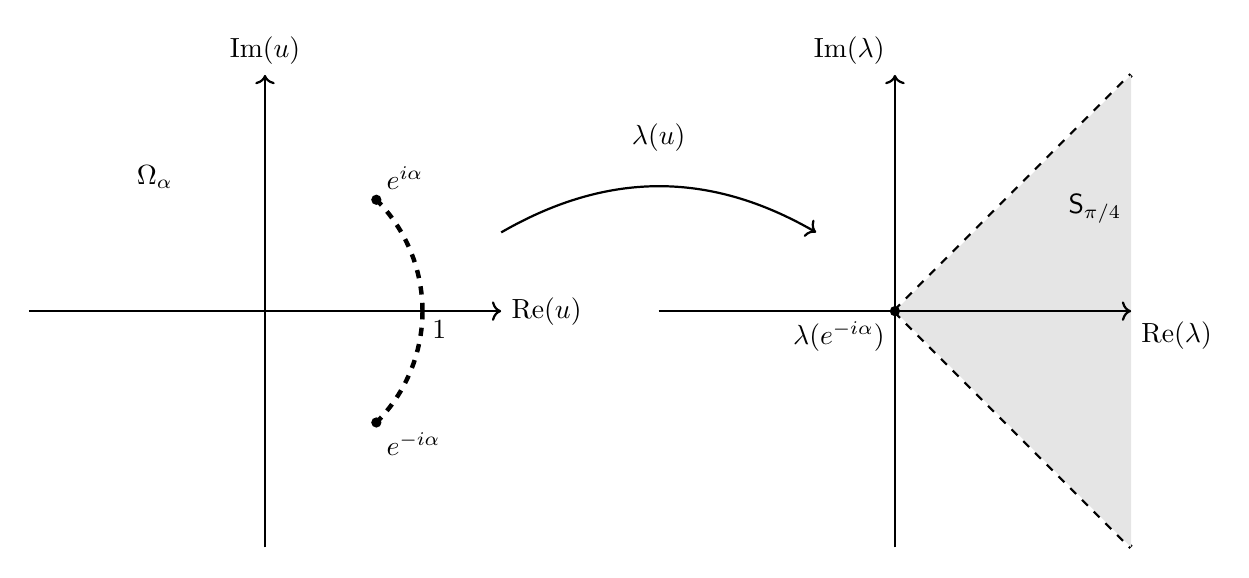
\begin{tikzpicture}

% Left: u-plane
\begin{scope}
	% Draw the dashed circular arcs
	\draw[dashed, ultra thick] (2,0) arc[start angle=0, end angle=45, radius=2];
    \draw[dashed, ultra thick] (2,0) arc[start angle=0, end angle=-45, radius=2];

    % Horizontal axis and labels
    \draw[thick, ->] (-3,0) -- (3,0) node[right] {$\text{Re}(u)$};
    \draw[thick, ->] (0,-3) -- (0,3) node[above] {$\text{Im}(u)$};
    
	% Points e^{i alpha} and e^{-i alpha}
	\draw[thick,fill=black] (1.4142135624,1.4142135624) circle(0.05)node[above right] {$e^{i\alpha}$};
    \draw[thick,fill=black] (1.4142135624,-1.4142135624) circle(0.05)node[below right] {$e^{-i\alpha}$};

    % Mark u=1 point
    \node[below right] at (2,0) {$1$};
	
    % Codomain label
    \node at (-1.4,1.7) {$\Omega_\alpha$};
\end{scope}

% Right: lambda-plane
\begin{scope}[xshift=8cm]
  % Draw the dashed lines
    \draw[dashed, ultra thick] (0,0) -- (3,3);
    \draw[dashed, ultra thick] (0,0) -- (3,-3);
    
    % Fill the region between the lines with light gray
    \fill[gray!20] (0,0) -- (3,3) -- (3,-3) -- cycle;
  	% Draw the lambda-plane
  	\draw[thick,->] (-3,0) -- (3,0) node[below right] {$\Re(\lambda)$};
  	\draw[thick,->] (0,-3) -- (0,3) node[above left] {$\Im(\lambda)$};

 	% Add labels for S_pi/4
  	\node[left,black] at (3,1.3) {$\mathsf{S}_{\pi/4}$};
  	\draw[thick,fill=black] (0,0) circle(0.05)node[below left] {$\lambda(e^{-i\alpha})$};
\end{scope}

\draw[->, thick] (3,1) to[out=30, in=150] (7,1);

% Map label
\node[above] at (5,1.9) {$\lambda(u)$};
\end{tikzpicture}	
\end{center}

%As is shown in \cite[Theorem 1.2]{eichinger17}, if $|u_0|<1$ and $P_{n,u_0}$ is extremal with respect to \eqref{eq:residual_extremal_value} where $w\equiv 1$, then there is a number $\phi\in [0,2\pi)$ such that
%\begin{equation}
%	\lim_{n\rightarrow \infty}b_{\Omega_\alpha}(u,\infty)^nP_{n,u_0}(u) = e^{i\phi}\frac{1}{2}\left(1+\frac{h(\lambda,\lambda_0)}{h(\lambda_0,\lambda_0)}\right)\frac{\lambda^2-|\lambda_0|^2}{\lambda^2+|\lambda_0|^2}\frac{\lambda^2+\lambda_0^2}{\lambda^2-\overline{\lambda}_0^2}
%	\label{eq:benjamin_formula}
%\end{equation}
%uniformly on compact subsets of $\Omega_\alpha$. The function $h$ is defined by
%\[h(\lambda,\lambda_0) = \frac{\lambda^2}{(\lambda^2-|\lambda_0|^2)(\lambda^2+|\lambda_0|^2)}.\]

First, we extend this result to weighted polynomials, where the weight is the multiplicative inverse of a polynomial. Ultimately, this will enable us to prove that for $u\in \Omega_\alpha$ and a general class of weights, whose properties are detailed in Theorem \ref{thm:main_norm_asymptotics},
%and as $n\to\infty$, 
\begin{equation}
	\|wT_n^{\Gamma_{\alpha},w}(\cdot ,u)\|_{\Gamma_\alpha} \sim e^{-ng_{\Omega_\alpha}(u,\infty)}k_{\C_+}\bigl(\lambda(u),\lambda(u)\bigr)^{-1}\exp\left(\int_{\Gamma_\alpha}\log w(x)\,\omega(u,dx,\Omega_{\alpha})\right).
	\label{eq:residual_norm_asymptotics}
\end{equation}
In the special case $u = \infty$, we obtain the asymptotic formula
\begin{equation}
	\lim_{n\rightarrow \infty}\frac{\|wT_n^{\Gamma_{\alpha},w}\|_{\Gamma_\alpha}}{\Cap(\Gamma_\alpha)^n}= 2\cos^2(\alpha/4)\exp\left(\int_{\Gamma_\alpha}\log w(x)\,d\mu_{\Gamma_\alpha}(x)\right).
	\label{eq:chebyshev_norm_asymptotics}
\end{equation}
This should be compared with the unweighted ($w\equiv 1$) asymptotic formula
\begin{equation}
\lim_{n\rightarrow \infty}\frac{\|T_n^{\Gamma_\alpha}\|_{\Gamma_\alpha}}{\Cap(\Gamma_\alpha)^n} = 2\cos^2(\alpha/4)
\end{equation}
that was derived in \cite{thiran-detaille91}. 
%A deeper understanding of the monotonicity properties of this convergence was later obtained through \cite[Theorem 8]{schiefermayr-zinchenko21}. This example is historically significant since it disproves a conjecture of Widom \cite{widom69}, claiming that for a sufficiently smooth Jordan arc \(\Gamma\), 
%%\begin{equation}
%%   \lim_{n\rightarrow \infty}\frac{\|T_n^{\Gamma}\|_{\Gamma}}{\Cap(\Gamma)^n}= 2.
%%\end{equation}
%Widom formulated this conjecture based on the interval case and the upper bound \eqref{eq:alpan_asymptotics} presented below. Let \( w:\Gamma\rightarrow [0,\infty) \) be a bounded upper semicontinuous function satisfying \( \log w \in L^1(\mu_\Gamma) \). Then, by \cite[Theorem 11.4]{widom69}, it follows that
%\begin{equation}
%\limsup_{n \to \infty} \frac{\|wT_n^{\Gamma,w}\|_{\Gamma}}{\Cap(\Gamma)^n} \leq 2\exp\left(\int_{\Gamma} \log w(x) \, d\mu_{\Gamma}(x)\right).
%\label{eq:alpan_asymptotics}
%\end{equation}
%Observe that in the unweighted case, the integral vanishes. 
A deeper understanding of the monotonicity properties of this convergence was later obtained through \cite[Theorem 8]{schiefermayr-zinchenko21}. The context for this result is historically significant. For a bounded upper semicontinuous function $w:\Gamma\rightarrow [0,\infty)$ with $\log w \in L^1(\mu_\Gamma)$, Widom established the general upper bound \cite[Theorem 11.4]{widom69}:
\begin{equation}
\limsup_{n \to \infty} \frac{\|wT_n^{\Gamma,w}\|_{\Gamma}}{\Cap(\Gamma)^n} \leq 2\exp\left(\int_{\Gamma} \log w(x) \, d\mu_{\Gamma}(x)\right).
\label{eq:alpan_asymptotics}
\end{equation}
In the unweighted case, the integral vanishes, reducing this bound to 2. Motivated by this and the known result for an interval, Widom conjectured that for any sufficiently smooth Jordan arc $\Gamma$, the limit would always be exactly 2, i.e., that $\lim_{n\rightarrow \infty}\|T_n^{\Gamma}\|_{\Gamma}/\Cap(\Gamma)^n = 2$. The example under discussion is notable because it was the first to disprove this conjecture.

In sharp contrast to Widom's conjecture, a recent result by Alpan \cite[Theorem 1.3]{alpan22} proves that the inequality in \eqref{eq:alpan_asymptotics} is strict if there is an interior point $z\in \Gamma$ (i.e., a point other than its endpoints) for which
\begin{equation}
\frac{\partial g_{\Omega_\Gamma}}{\partial n_+}(z,\infty) \neq \frac{\partial g_{\Omega_\Gamma}}{\partial n_-}(z,\infty), \quad \Omega_\Gamma = \RS\setminus \Gamma.
\label{eq:not-s-property-arc}
\end{equation}
Here, the normal derivatives are taken with respect to the two different sides of the arc. As later observed in \cite[Theorem 1.1]{christiansen-eichinger-rubin23}, the only arc for which equality in \eqref{eq:not-s-property-arc} holds at all interior points is a straight line segment, which therefore constitutes the sole arc where Widom's conjecture is valid.

%Widom based his conjecture on the case of an interval; however, as a result by Alpan \cite{alpan22} shows,
%\begin{equation}
%\limsup_{n \to \infty} \frac{\|wT_n^{\Gamma,w}\|}{\Cap(\Gamma)^n} \leq 2\exp\left(\int_{\Gamma} \log w(\zeta) \, d\mu_{\Gamma}(\zeta)\right),
%\label{eq:alpan_asymptotics}
%\end{equation}
%with equality if and only if
%\begin{equation}
%\frac{\partial g_{\Omega_\Gamma}}{\partial n_+}(z,\infty) = \frac{\partial g_{\Omega_\Gamma}}{\partial n_-}(z,\infty)
%\label{eq:s-property-arc}
%\end{equation}
%holds at every interior point \( z \in \Gamma \). Here, the normal derivatives are taken with respect to the two different sides of the arc. The weight function \( w \) is assumed to be a bounded upper semicontinuous function such that \( \log w \in L^1(\mu_\Gamma) \). As later observed in \cite{christiansen-eichinger-rubin23}, the only arc for which \eqref{eq:s-property-arc} holds at all interior points is a straight-line segment which therefore constitutes the only possible arc for which Widom's conjecture is valid.

When it comes to lower bounds, we may also consider %any compact set $\E$ of positive capacity and 
any weight function \( w: \E \to [0,\infty) \) for which \( \log w \in L^1(\mu_\E) \). In this case, Szeg\H{o}'s inequality holds:
\begin{equation}
\|wT_n^{\E,w}\|_{\E} \geq \Cap(\E)^n \exp\left(\int_{\E} \log w(x) \, d\mu_\E(x)\right),
\label{eq:szego_inequality}
\end{equation}
as shown in \cite[Theorem 13]{novello-schiefermayr-zinchenko21}. Based on \eqref{eq:alpan_asymptotics} and \eqref{eq:szego_inequality}, it is natural to introduce the \emph{weighted Widom factors} as
\begin{equation}
\mathcal{W}_n(\E,w) := \frac{\|wT_n^{\E,w}\|_{\E}}{\Cap(\E)^n}.
\label{eq:widom_factor}
\end{equation}
%where \( w: \E \to [0,\infty) \) is a weight function. 
The unweighted Widom factors, corresponding to $w\equiv 1$, will be denoted by $\cW_n(\E)$. For an arc \( \Gamma \), combining \eqref{eq:alpan_asymptotics} and \eqref{eq:szego_inequality} implies that all limit points of \( \mathcal{W}_n(\Gamma,w) \) lie within the range
\begin{equation}
	\left[\exp\left(\int_{\Gamma} \log w(x) \, d\mu_{\Gamma}(x)\right), 2\exp\left(\int_{\Gamma} \log w(x) \, d\mu_{\Gamma}(x)\right)\right].
	\label{eq:upper_lower_bounds_widom_factors}
\end{equation}
%This should be compared with the unweighted asymptotical formula
%\[\|T_n^{\Gamma_\alpha}\|_{\Gamma_\alpha}\sim 2\cos^2(\alpha/4)\Cap(\Gamma_\alpha)^n\]
%as $n\rightarrow \infty$, which was derived in \cite{thiran-detaille91}. More precise asymptotics were subsequently obtained in \cite{schiefermayr-zinchenko21}. This example has historical significance since it disproves a conjecture of Widom \cite{widom69} which entailed that if $\Gamma$ is a Jordan arc then 
%\[\|T_n^{\Gamma}\|_{\Gamma}\sim 2\Cap(\Gamma)^n\]
%as $n\rightarrow \infty$. Widom bases his conjecture on the case of an interval, however, as a result of Alpan \cite{alpan22} shows
%\begin{equation}
%	\limsup_{n\rightarrow \infty}\|wT_n^{\Gamma,w}\|/\Cap(\Gamma)^n\leq 2\exp\left(\int_{\Gamma}\log w(\zeta)d\mu_{\Gamma}(\zeta)\right)
%	\label{eq:alpan_asymptotics}
%\end{equation}
%with equality if and only if
%\begin{equation}
%	\frac{\partial g_{\Omega_\Gamma}}{\partial n_+}(z,\infty)=\frac{\partial g_{\Omega_\Gamma}}{\partial n_-}(z,\infty)
%	\label{eq:s-property-arc}
%\end{equation}
%holds at every interior point $z\in \Gamma$. The normal derivatives are taken with respect to the two different sides of the arc. The requirements of the weight function $w$ is that it is a bounded upper semicontinuous function such that $\log w$ belongs to $L^1(\mu_\Gamma)$. As is later observed in \cite{christiansen-eichinger-rubin23} the only arc for which \eqref{eq:s-property-arc} holds at all interior point are straight-line segments. In the other direction, for any compact set with positive capacity and weight function $w:\E\rightarrow [0,\infty)$ such that $\log w\in L^1(\mu_\E)$ Szeg\H{o}'s inequality is valid, which says that
%\begin{equation}
%	\|wT_n^{\E,w}\|_{\\E}\geq \Cap(\E)^n\exp\left(\int_{\E}\log w(\zeta)d\mu_\E(\zeta)\right),
%	\label{eq:szego_inequality}
%\end{equation}
%see \cite[Theorem 13]{novello-schiefermayr-zinchenko21}. It is therefore natural to introduce the weighted Widom factors
%\begin{equation}
%	\cW_n(\E,w):=\frac{\|wT_n^{\E,w}\|_{\E}}{\Cap(\E)^n},
%	\label{eq:widom_factor}	
%\end{equation}
%where $w:\E\rightarrow [0,\infty)$ is a weight function. In the case of an arc $\Gamma$ the combination of \eqref{eq:alpan_asymptotics} and \eqref{eq:szego_inequality} implies that all limit points of $\cW_n(\Gamma,w)$ lie within 
%\[\left[\exp\left(\int_{\Gamma}\log w(\zeta)d\mu_{\Gamma}(\zeta)\right),2\exp\left(\int_{\Gamma}\log w(\zeta)d\mu_{\Gamma}(\zeta)\right)\right].\]
We emphasize that exact formulas for limit points of the Widom factors %$\{\cW_n(\Gamma,w)\}$ 
associated with arcs are scarce in the literature. Notably, the case of an interval remains the only thoroughly studied example, largely due to the seminal work of Bernstein \cite{bernstein30, bernstein31}. For the norms of unweighted Chebyshev polynomials relative to an arc, the only case understood beyond an interval is that of a circular arc.
%
%Progressively, throughout this text, the regularity assumptions on the weight function $w$ will be relaxed. For sufficiently simple weights, we can derive more precise asymptotics, known as Szeg\H{o}--Widom asymptotics, a name originating with \cite{christiansen-simon-zinchenko-I}. For less regular weights, however, we limit ourselves to determining asymptotic formulas, such as \eqref{eq:chebyshev_norm_asymptotics}. This type of results culminate in Theorem \ref{thm:main_norm_asymptotics}. Our approach mirrors that of Bernstein \cite{bernstein30,bernstein31}, where extremal polynomials on the unit interval were investigated.

%We wish to highlight the greater challenge in deriving the asymptotics of Chebyshev polynomials for Jordan arcs compared to Jordan curves. The main reason for this is that weighted Chebyshev polynomials do not asymptotically saturate the lower bounds which are typically obtained through a study of conformal mappings in conjunction with the maximum principle, see \cite[Theorem 1]{totik14}. This also explains why care must be taken in the consideration of relaxing weight properties such as regularity and positivity. In the case of Jordan curves, as studied in \cite{widom69}, extending results from smooth, non-vanishing weights to vanishing weights with minimal regularity can be achieved by approximating weights from above and comparing with lower bounds. However, such an approach is no longer feasible in the context of Jordan arcs. To the best of our knowledge, Theorem \ref{thm:main_norm_asymptotics} is the first result to present asymptotic formulas for $\|w T_n^{\E,w}\|_\E$ when $\E$ is an arc distinct from $[-1,1]$ and $w$ is a general positive weight.

%Given a bounded weight function $w:\Gamma_\alpha\rightarrow [0,\infty)$, with associated Chebyshev polynomials $T_n^w$, we ultimately wish to show versions of the asymptotic formula
%\begin{equation}
%	\|w T_n^w\|_{\Gamma_\alpha}\sim 2\cos(\alpha/4)^2\sin(\alpha/2)^n\exp\left(\int_{-\alpha}^{\alpha}\log w(e^{ix})\frac{\cos(x/2)}{2\pi\sqrt{\sin^2(\alpha/2)-\sin^2(x/2)}}dx\right\)
%	\label{eq:chebyshev_norm_asymptotics}
%\end{equation}
%as $n\rightarrow \infty$. When writing $f(n)\sim g(n)$ as $n\rightarrow \infty$, we mean that $f(n)/g(n)\rightarrow 1$ as $n\rightarrow \infty$. Note that the density
%\[d\mu_{\Gamma_\alpha}(x):=\frac{\cos(x/2)}{2\pi\sqrt{\sin^2(\alpha/2)-\sin^2(x/2)}}dx\] 
%on $\Gamma_\alpha$ is nothing but the density of the potential theoretic equilibrium measure, while $\sin(\alpha/2)$ coincides with the logarithmic capacity of $\Gamma_\alpha$. Thiran and Detaille demonstrated in \cite{thiran-detaille91} that in the unweighted case, the following asymptotic relation holds:
%\[\|T_n^{\Gamma_\alpha}\|_{\Gamma_{\alpha}}\sim 2\cos^2(\alpha/4)\sin(\alpha/2)^n\]
%as $n\rightarrow \infty$. Therefore \eqref{eq:chebyshev_norm_asymptotics} can be seen as an extension of their result.

%Consequently, we can give more precise asymptotics, called Szeg\H{o}-Widom asymptotics in \cite{christiansen-simon-zinchenko-I}, for simple enough weights while we contempt ourselves with determining asymptotical formulas such as \eqref{eq:chebyshev_norm_asymptotics} for less regular weights. This is similar to Bernstein's approach found in \cite{bernstein30,bernstein31} where extremal polynomials on the unit interval were studied. 

Exploring the implications of the results presented here, as well as those in \cite{eichinger17}, for analyzing convergence rates of Krylov subspace methods would be interesting but lies beyond the scope of this article. In particular, it would be of interest to investigate algorithms related to unitary matrices with restricted spectra. %However, given the numerical nature of these considerations, we have chosen not to include this in the present discussion.
However, due to the numerical nature of such considerations, we have opted not to include them in the present discussion.

\subsection{Outline}
In Section \ref{sec:chebyshev_polynomials_system_of_arcs}, we analyze the asymptotic behavior of the norms of Chebyshev polynomials associated with subsets of $\{z:|z^m+1| = r\}$ for $r>0$. %symmet defined by \(\{z: z^m+1 \in r\Gamma_\alpha\}\), where \(m \in \mathbb{Z}_+\), \(0 < r < \infty\), and \(0 < \alpha<\pi\). 
Our complete asymptotic analysis is collected in Theorem \ref{thm:Widom_factors_lemniscatic_arcs} which relies on the weighted formulas proven in Section \ref{sec:general_weight}. One of our goals is to analyze the effects of \eqref{eq:not-s-property-arc} on the potential limit points of the Widom factors for a connected system of arcs.

%One of our aims is to attempt to analyze the effects of \eqref{eq:not-s-property-arc} on the possible limit points of the Widom factors for a connected system of arcs.

In Section \ref{sec:reciprocal_weight}, we will adopt the approach from \cite{eichinger17} where Szeg\H{o}--Widom asymptotics is established for circular arcs in the general residual polynomial setting. In fact, we will provide similar results for weight functions which are given as reciprocals of polynomials. To be more precise, in Theorem %\ref{thm:szego_widom_asymptotics} 
\ref{thm:weighted_residual_asymptotics} we determine the asymptotic behavior of 
%\[
   $R_n^{\Gamma_\alpha,1/P}(\cdot, u)$
%\]    
%in $\Omega_\alpha$ 
when $P$ is a polynomial which does not vanish on the unit circle. 
This result enables us to determine the asymptotic behavior of 
%\[
   $\|T_n^{\Gamma_\alpha,1/P}(\cdot,u)/P\|_{\Gamma_\alpha}$
%\]    
in Theorem \ref{thm:weighted_residual_asymptotics_at_point}, which serves as the foundation for the work presented in Section \ref{sec:general_weight}. There, we determine the asymptotic behavior of \(\|wT_n^{\Gamma_\alpha,w}(\cdot,u)\|_{\Gamma_\alpha}\), with a particular focus on the case \(u=\infty\), for a general class of weight functions, including those that may vanish on $\Gamma_\alpha$. Specifically, Theorem \ref{thm:main_norm_asymptotics} generalizes the results of Bernstein \cite{bernstein30,bernstein31}, who studied the asymptotic behavior of $\|wT_n^{[-1,1],w}\|_{[-1,1]}$ for general weight functions $w:[-1,1]\rightarrow [0,\infty)$.


\section{Chebyshev polynomials on lemniscatic arcs}
\label{sec:chebyshev_polynomials_system_of_arcs}
To illustrate the applicability of Theorem \ref{thm:main_norm_asymptotics}, we derive asymptotic formulas for the Widom factors associated with a family of unions of arcs. These results complement the analysis in \cite{christiansen-eichinger-rubin23}. 

As previously mentioned, when $\Gamma$ is a smooth arc,
\[
\limsup_{n \to \infty} \cW_n(\Gamma, w) \leq 2 \exp\left(\int_{\Gamma} \log w(x) \, d\mu_\Gamma(x)\right),
\] 
with equality if and only if $\Gamma$ is a straight line segment. This result is rooted in the fact that a straight line segment is the only Jordan arc \(\Gamma\) satisfying 
\begin{equation} 
\frac{\partial g_{\Omega_\Gamma}}{\partial n_+}(z,\infty) = \frac{\partial g_{\Omega_\Gamma}}{\partial n_-}(z,\infty), \quad \Omega_\Gamma = \RS\setminus \Gamma
\label{eq:s-property-arc}
\end{equation} 
at all interior points. The generalization of \eqref{eq:s-property-arc} to a system of arcs is given by the $S$-property, which is formally defined below in Definition \ref{def:s-property}.

The results of \cite{christiansen-eichinger-rubin23} suggest that the $S$-property is the key mechanism behind large limits of Widom factors, specifically leading to a limit of 2. In this section, we provide further evidence for this by examining a family of unions of arcs where the $S$-property fails and show that their corresponding Widom factors are asymptotically strictly less than 2.

\subsection{Main Result}
Extremal polynomials on lemniscates have been extensively studied, particularly for sets of the form $\{z:z^m+1\in r\T\}$ (see e.g. \cite{bergman-rubin24, peherstorfer-steinbauer01, minadiaz06, ullman60, he94}). To obtain a system of arcs from this structure, we consider the pre-image of a circular arc rather than a full circle:
\begin{equation}
	\E_{m,r}(\alpha):=\{z: z^m+1\in r \Gamma_\alpha\},\quad 0<\alpha<\pi,
	\label{eq:def_lemniscatic_arc}
\end{equation}
where $m\in \N$ and $r>0$. The geometry of these sets depends critically on the parameter $r$. The sets in \eqref{eq:def_lemniscatic_arc} consist of \(m\) disjoint analytic arcs when \(r \neq 1\). However, if \(r = 1\), the components connect at the origin, where \(2m\) analytic arcs meet. Examples of these structures are shown in Figure \ref{fig:system_arcs}.

\begin{figure}[htbp]
    \centering
    \begin{subfigure}[t]{0.32\textwidth}
        \centering
        \includegraphics[width=0.8\textwidth]{Figures/m2_2.pdf} % replace with your figure
        \caption{\(\E_{2,1}(\pi/7)\)}
    \end{subfigure}
    \hfill
    \begin{subfigure}[t]{0.32\textwidth}
        \centering
        \includegraphics[width=\textwidth]{Figures/m5_2.pdf} % replace with your figure
        \caption{\(\E_{5,1}(\pi/7)\)}
    \end{subfigure}
    \hfill
    \begin{subfigure}[t]{0.32\textwidth}
        \centering
        \includegraphics[width=\textwidth]{Figures/m7_2.pdf} % replace with your figure
        \caption{\(\E_{7,1}(\pi/7)\)}
    \end{subfigure}
    \begin{subfigure}[t]{0.32\textwidth}
        \centering
        \includegraphics[width=0.8\textwidth]{Figures/m2_1.pdf} % replace with your figure
        \caption{\(\E_{2,0.9}(\pi/7)\) and \(\E_{2,1.1}(\pi/7)\)}
    \end{subfigure}
    \hfill
    \begin{subfigure}[t]{0.32\textwidth}
        \centering
        \includegraphics[width=\textwidth]{Figures/m5_1.pdf} % replace with your figure
        \caption{\(\E_{5,0.9}(\pi/7)\) and \(\E_{5,1.1}(\pi/7)\)}
    \end{subfigure}
    \hfill
    \begin{subfigure}[t]{0.32\textwidth}
        \centering
        \includegraphics[width=\textwidth]{Figures/m7_1.pdf} % replace with your figure
        \caption{\(\E_{7,0.9}(\pi/7)\) and \(\E_{7,1.1}(\pi/7)\)}
    \end{subfigure}

    \caption{Examples of sets in the families $\E_{2,r}(\pi/7)$, $\E_{5,r}(\pi/7)$ and $\E_{7,r}(\pi/7)$ for varying values of $r$. The lines corresponding to \(r=1.1\) are dashed.}
    \label{fig:system_arcs}
\end{figure}
%\begin{figure}[h!]
%	\centering
%	\includegraphics[width = \textwidth]{Figures/system_arcs.png}
%	\caption{Examples of sets in the families $\E_{2,r}(\pi/7)$, $\E_{5,r}(\pi/7)$ and $\E_{7,r}(\pi/7)$ for varying values of $r$. The critical case $r = 1$, where the arcs connect, is marked with a solid line.}
%	\label{fig:system_arcs}
%\end{figure}

Our main result provides the explicit limit of the Widom factors for this family of sets.

\begin{theorem} 	
\label{thm:Widom_factors_lemniscatic_arcs}
	Let $\E_{m,r}(\alpha)=\{z: z^m+1\in r \Gamma_\alpha\}$, where $m\in \N$, $r>0$, and $0<\alpha<\pi$. Then, for any $0\leq l <m$, we have
\begin{equation}
   \lim_{n\rightarrow \infty}\cW_{nm+l}\bigl(\E_{m,r}(\alpha)\bigr) = 2\cos^2(\alpha/4)\, c(r,\alpha)^{l/m}
\end{equation} 	
	where
\begin{equation}
\label{eq:c_r_alpha_definition}
c(r,\alpha)=\frac{\vert 1-r \vert + \sqrt{1-2r\cos(\alpha)+r^2}}{2r\sin(\alpha/2)}.
%\frac{\frac{r^2+1}{2}-r\cos^2(\alpha/2)+\sqrt{\left(\frac{r^2+1}{2}-r\cos^2(\alpha/2)\right)^2-r^2\sin^4(\alpha/2)}}{r^2\sin^2(\alpha/2)}.
\end{equation}
	In particular, for the connected case where $r = 1$, we have
\begin{equation}
\label{eq:widom_limit_r_1}
\lim_{n\rightarrow \infty}\cW_n\bigl(\E_{m,1}(\alpha)\bigr) = 2\cos^2(\alpha/4).
\end{equation}
\end{theorem}

This theorem is significant because, as we will show in Proposition \ref{prop:no_s_property}, the connected set $\E_{m,1}(\alpha)$ does not satisfy the $S$-property. The explicit formula \eqref{eq:widom_limit_r_1} demonstrates that this absence of the $S$-property leads to a limit strictly less than 2, supporting the conjecture that the $S$-property is essential for Widom factors of connected sets to approach 2.

\subsection{Proof of Theorem \ref{thm:Widom_factors_lemniscatic_arcs}}
The proof proceeds in several steps. First, we formally define the $S$-property and prove that the set $\E_{m,1}(\alpha)$ does not possess it. Second, we use symmetry arguments to reduce the problem to an analysis of weighted Chebyshev polynomials on the circular arc $\Gamma_\alpha$. Finally, we compute the necessary potential-theoretic quantities to derive the asymptotic formula.

We begin with the formal definition.
\begin{definition}%[S-property]
\label{def:s-property}
    Let $\E\subset \C$ be a compact set with $\Cap(\E)>0$, and suppose that $\Omega_\E=\RS\setminus \E$ is connected. Additionally, assume there exists a subset $\E_0\subset \E$ with $\Cap(\E_0) = 0$, such that
    \begin{equation}
    	\E\setminus \E_0 = \bigcup_{i\in I}\Gamma_i,
    \end{equation}
    where the $\Gamma_i$'s are disjoint open analytic Jordan arcs, and $I\subset \N$. We say that $\E$ satisfies the \emph{$S$-property} if
    \begin{equation}
		\frac{\partial g_{\Omega_\E}}{\partial n_+}(z,\infty)=\frac{\partial g_{\Omega_\E}}{\partial n_-}(z,\infty)
		\label{eq:s-property}
	\end{equation}
    holds for all $z\in \E\setminus \E_0$, where $n_+$ and $n_-$ denote the unit normals from each side of the arcs.
\end{definition}

The \(S\)-property is closely related to capacity minimization, and we refer the reader to \cite{stahl85-1,stahl85-2,stahl12} for further details on this. In \cite{christiansen-eichinger-rubin23}, the Chebyshev polynomials associated with the $m$-stars defined by $\E_m:=\{z:z^m\in [-2,2]\}$ are studied. These $m$-stars serve as examples of sets with the $S$-property, and it is shown that $\cW_n(\E_m)\rightarrow 2$ as $n\rightarrow \infty$ for any $m$. This behavior is analogous to that of Jordan arcs satisfying the $S$-property (i.e., straight line segments).

%We now show that our set of interest fails this property. 
In order to show that $\E_{m,1}(\alpha)$ does not satisfy \eqref{eq:s-property} at interior points of the subarcs, we utilize the connection to Chebotarev sets. Given $N$ distinct points $a_1\dotsc,a_N$ in the complex plane, there is a unique continuum (i.e., a compact connected set) of minimal logarithmic capacity containing these points. This set is known as the Chebotarev set for $\{a_1,\ldots,a_N\}$, with relevant references detailing its properties found in \cite{stahl12, grotzsch30, schiefermayr14, schiefermayr15, kuzmina80, fedorov85, martinez-finkelshtein-rakhmanov11, ortega-cerda-pridhnani08}. 
It is known (see \cite{stahl12}) that every Chebotarev set necessarily has the form specified in Definition \ref{def:s-property} and therefore satisfies the $S$-property. Conversely, a compact set with the specified structure of analytic arcs that satisfies the $S$-property must be the Chebotarev set for some finite collection of points, as can be inferred from the discussion following Problem 2 and Theorem 11 in \cite{stahl12}.
%It is known (see \cite{stahl12}) that every Chebotarev set necessarily has the form specified in Definition \ref{def:s-property} and therefore satisfies the $S$-property. Moreover, the converse also holds, as can be inferred from the discussion following Problem 2 and Theorem 11 in \cite{stahl12}. 
In our case, this implies the following: if $\E_{m,1}(\alpha)$ were to satisfy \eqref{eq:s-property} away from the points \(\{0\}\cup\{z: z^m+1\in e^{\pm i \alpha}\}\), it would necessarily coincide with the Chebotarev set associated with these points, excluding the point at zero.

\begin{proposition}
\label{prop:no_s_property}
For $0<\alpha<\pi$ and $m\in \N$, the set $\E_{m,1}(\alpha)$, as defined in \eqref{eq:def_lemniscatic_arc}, does not satisfy the $S$-property.
\end{proposition}
\begin{proof}
The proof is carried out by showing that $\E_{m,1}(\alpha)$ is \emph{not} the Chebotarev set for the points $\{z:z^m+1\in e^{\pm i\alpha}\}$. %A Chebotarev set has minimal capacity among all continua containing a given set of points and is known to satisfy the $S$-property.
To see this, let $\mathcal{C}(e^{\pm i\alpha}, 1)$ denote the Chebotarev set for $\{e^{\pm i\alpha}, 1\}$. By \cite[Theorem 1.2]{kuzmina80}, this set is necessarily contained within the convex hull of these points. Since this does not hold for $\Gamma_\alpha$, we conclude that $\Gamma_\alpha\neq \mathcal{C}(e^{\pm i\alpha},1)$, which in turn implies 
\[
\Cap(\Gamma_\alpha)>\Cap\bigl(\mathcal{C}(e^{\pm i\alpha},1)\bigr).
\] 
Furthermore, the set $\{z: z^m+1\in \mathcal{C}(e^{\pm i\alpha}, 1)\}$ forms a continuum (since $\mathcal{C}(e^{\pm i\alpha}, 1)$ contains the critical value of $z^m+1$). Applying \cite[Theorem 5.2.5]{ransford95} twice, we obtain
\[
\Cap\bigl(\{z:z^m+1\in \mathcal{C}(e^{\pm i\alpha},1)\}\bigr) = 
\Cap\bigl(\mathcal{C}(e^{\pm i\alpha},1)\bigr)^{1/m} < 
\Cap(\Gamma_\alpha)^{1/m} = 
\Cap\bigl(\E_{m,1}(\alpha)\bigr).
\]
Thus, \(\E_{m,1}(\alpha)\) is not the minimal capacity set containing \(\{z:z^m+1\in e^{\pm i\alpha}\}\) and consequently does not satisfy the $S$-property.
\end{proof}

%Having established that $\E_{m,1}(\alpha)$ lacks the S-property, we proceed with the main asymptotic calculation for the Widom factors. The argument exploits the rotational symmetry of $\E_{m,r}(\alpha)$. This set is invariant under rotation by $2\pi/m$ radians, implying the Chebyshev polynomial $T_{nm+l} := T_{nm+l}^{\E_{m,r}(\alpha)}$ satisfies $T_{nm+l}(e^{2\pi i/m}z) = e^{2\pi il/m} T_{nm+l}(z)$. Consequently, $T_{nm+l}(z) = z^l Q_n(z^m+1)$ for some monic polynomial $Q_n$ of degree $n$.
%Via the change of variables $z = (r\zeta-1)^{1/m}$, we relate the norm on $\E_{m,r}(\alpha)$ to a weighted norm on $\Gamma_\alpha$. Let $w_{r,m,l}(\zeta) := |r\zeta-1|^{l/m}$. Then $Q_n(r\zeta) = r^n \tilde{Q}_n(\zeta)$, where $\tilde{Q}_n$ is the monic polynomial minimizing $\| w_{r,m,l} \tilde{Q}_n \|_{\Gamma_\alpha}$. Thus, $\tilde{Q}_n = T_n^{\Gamma_\alpha, w_{r,m,l}}$, and
%\[
%\|T_{nm+l}\|_{\E_{m,r}(\alpha)} = r^n \|w_{r,m,l} T_n^{\Gamma_\alpha, w_{r,m,l}}\|_{\Gamma_\alpha}.
%\]
%The asymptotics of the weighted norm are given by Theorem \ref{thm:main_norm_asymptotics}:
%\begin{equation}
%\label{eq:cheb_on_lemniscatic_arcs_weight_asymptotics_streamlined} % Renamed label for clarity
%\|w_{r,m,l} T_n^{\Gamma_\alpha, w_{r,m,l}}\|_{\Gamma_\alpha} \sim 2\cos^2(\alpha/4) \Cap(\Gamma_\alpha)^n \exp\left(\int_{\Gamma_\alpha} \log w_{r,m,l}(\zeta) \, d\mu_{\Gamma_\alpha}(\zeta)\right).
%\end{equation}
%The integral term is $I = \frac{l}{m} \int_{\Gamma_\alpha} \log|r\zeta-1| \, d\mu_{\Gamma_\alpha}(\zeta)$. For $r \neq 1$, this integral equals $\frac{l}{m} h_r(\infty)$, where $h_r$ solves the Dirichlet problem on $\Omega_\alpha := \overline{\C}\setminus\Gamma_\alpha$ with boundary data $\log|r\zeta-1|$. From potential theory \cite[Thm 4.3.14]{ransford95}, $h_r(\infty) = \log r + \log\Cap(\Gamma_\alpha) + g_{\Omega_\alpha}(1/r,\infty)$. The Green's function $g_{\Omega_\alpha}(z,\infty)$ can be found using the conformal map $f(z) = \frac{1}{2} ( z-1+\sqrt{z^2-2z\cos(\alpha)+1} )$ from $\Omega_\alpha$ onto $\{w : |w| > \sin(\alpha/2)\}$ (cf. \cite[Exercise 5.2.4]{ransford95}), yielding $g_{\Omega_\alpha}(z, \infty) = \log(|f(z)|/\sin(\alpha/2))$. Evaluating at $z=1/r$ gives
%\begin{equation}
%\label{eq:green_at_1_over_r_direct}
%g_{\Omega_\alpha}(1/r, \infty) = \log\left( \frac{|1-r| + \sqrt{1-2r\cos(\alpha)+r^2}}{2r\sin(\alpha/2)} \right).
%\end{equation}
%Notice that the argument of the logarithm is precisely $c(r,\alpha)$ as defined in \eqref{2.4}. Thus, $g_{\Omega_\alpha}(1/r, \infty) = \log c(r,\alpha)$, and
%\[
%I = \frac{l}{m} h_r(\infty) = \frac{l}{m} \left( \log r + \log(\sin(\alpha/2)) + \log c(r,\alpha) \right) = \frac{l}{m} \log\left( r \sin(\alpha/2) c(r,\alpha) \right).
%\]
%Substituting this value for the integral into \eqref{eq:cheb_on_lemniscatic_arcs_weight_asymptotics_streamlined}, and using the capacity formula $\Cap(\E_{m,r}(\alpha)) = (r\Cap(\Gamma_\alpha))^{1/m} = (r\sin(\alpha/2))^{1/m}$, we find the limit of the Widom factors:
%\begin{align*}
%\lim_{n\to\infty} \cW_{nm+l}(\E_{m,r}(\alpha)) &= \lim_{n\to\infty} \frac{r^n \|w_{r,m,l} T_n^{\Gamma_\alpha, w_{r,m,l}}\|_{\Gamma_\alpha}}{(r\sin(\alpha/2))^{(nm+l)/m}} \\
%&= \lim_{n\to\infty} \frac{r^n \cdot 2\cos^2(\alpha/4)\sin^n(\alpha/2) \exp(I)}{r^{n+l/m}\sin^{n+l/m}(\alpha/2)} \\
%&= \frac{2\cos^2(\alpha/4)}{r^{l/m}\sin^{l/m}(\alpha/2)} \exp\left( \frac{l}{m} \log\left( r \sin(\alpha/2) c(r,\alpha) \right) \right) \\
%&= \frac{2\cos^2(\alpha/4)}{r^{l/m}\sin^{l/m}(\alpha/2)} \left( r \sin(\alpha/2) c(r,\alpha) \right)^{l/m} \\
%&= 2\cos^2(\alpha/4) c(r,\alpha)^{l/m}.
%\end{align*}
%This completes the proof of Theorem \ref{thm:Widom_factors_lemniscatic_arcs}. \qed

Having established that $\E_{m,1}(\alpha)$ lacks the S-property, we now proceed with the main asymptotic calculation for the Widom factors. The argument begins by exploiting the rotational symmetry of the set $\E_{m,r}(\alpha)$. This set is invariant under rotations by $2\pi/m$-radians. As a result, the corresponding Chebyshev polynomial of degree $nm + l$, where $0 \leq l < m$, satisfies the symmetry relation 
\[
T_{nm+l}^{\E_{m,r}(\alpha)}(e^{2\pi i/m}z) = e^{2\pi il/m} T_{nm+l}^{\E_{m,r}(\alpha)}(z).
\]
This implies that $T_{nm+l}^{\E_{m,r}(\alpha)}(z) = z^lQ_n(z^m+1)$, where $Q_n$ is a monic polynomial of degree $n$. By applying the change of variables $z = (r\zeta-1)^{1/m}$, we find that $Q_n(r\zeta) = r^n\tilde{Q}_n(\zeta)$, where $\tilde{Q}_n$ is the monic polynomial of degree $n$ that minimizes the norm on $\Gamma_\alpha$ with respect to the weight function $w_{r,m,l}(\zeta) = |r\zeta-1|^{l/m}$. In other words, $\tilde{Q}_n(\zeta) = T_{n}^{\Gamma_\alpha, w_{r,m,l}}(\zeta)=:T_{n}^{w_{r,m,l}}(\zeta)$, and
\[
\|T_{nm+l}^{\E_{m,r}(\alpha)}\|_{\E_{m,r}(\alpha)} = r^n\|w_{r,m,l}T_n^{w_{r,m,l}}\|_{\Gamma_\alpha}.
\]
The asymptotic behavior of the right-hand side is given by Theorem \ref{thm:main_norm_asymptotics}, which yields
\begin{equation}
	\|w_{r,m,l}T_n^{w_{r,m,l}}\|_{\Gamma_\alpha}\sim 2\cos(\alpha/4)^2\Cap(\Gamma_\alpha)^n\exp\left(\int_{\Gamma_\alpha}\log w_{r,m,l}(\zeta)\,d\mu_{\Gamma_\alpha}(\zeta)\right).
	\label{eq:cheb_on_lemniscatic_arcs_weight_asymptotics}
\end{equation}
To apply this formula, we must evaluate the integral in the exponential term, which is given by the following lemma.
\begin{lemma}
\label{lem:logarithmic_integral}
For $r>0$, the logarithmic potential is given by the identity
\begin{equation}
\label{2.9}
\int_{\Gamma_\alpha}\log |r\zeta-1| \, d\mu_{\Gamma_\alpha}(\zeta) = 
\log\left(\frac{\vert 1-r \vert + \sqrt{1-2r\cos(\alpha)+r^2}}{2}\right).
\end{equation}
%In particular, 
%\[
%\exp\left(\int_{\Gamma_\alpha}\log w_{r,m,l}(\zeta)\,d\mu_{\Gamma_\alpha}(\zeta)\right)
%=r\sin(\alpha/2)\,c(r,\alpha),
%\]
%where $c(r,\alpha)$ is defined in \eqref{eq:c_r_alpha_definition}.
\end{lemma}

\begin{proof}
%The case $r=1$ follows directly from Frostman's theorem \cite[Theorem 3.3.4]{ransford95} and the fact that $\Cap(\Gamma_\alpha) = \sin(\alpha/2)$. % and $c(1,\alpha)=1$.
%
%For $r\neq 1$, the integral equals $h_r(\infty)$, where $h_r$ solves the Dirichlet problem on $\Omega_\alpha = \overline{\C}\setminus\Gamma_\alpha$ with boundary data $\log|r\zeta-1|$. Standard potential theory yields %\cite[Thm 4.3.14]{ransford95}
%\begin{equation}
%\label{eq:hr_infinity_green_concise}
%h_r(\infty) = \log r + \log\Cap(\Gamma_\alpha) + g_{\Omega_\alpha}(1/r,\infty),
%\end{equation}
%where $g_{\Omega_\alpha}(z,\infty)$ is the Green's function of the exterior of $\Gamma_\alpha$. Using the fact that 
%\[
%f(z) = \frac{1}{2} \Bigl( z-1+\sqrt{ (z-e^{i\alpha})(z-e^{-i\alpha}) } \,\Bigr)
%\] 
%maps $\Omega_\alpha$ conformally onto $\{w : |w| > \sin(\alpha/2)\}$ (cf. \cite[Exercise 5.2.4]{ransford95}), we get the explicit formula $g_{\Omega_\alpha}(z, \infty) = \log\left({|f(z)|}/{\sin(\alpha/2)}\right)$.
%Evaluating at $z=1/r$ gives
%\begin{equation}
%g_{\Omega_\alpha}(1/r, \infty) %\log\left( \frac{|f(1/r)|}{\sin(\alpha/2)} \right)
%=\log\left( \frac{\vert 1-r \vert + \sqrt{1-2r\cos(\alpha)+r^2}}{2r\sin(\alpha/2)} \right) 
%=\log c(r,\alpha),
%\end{equation}
%where $c(r,\alpha)$ is defined in \eqref{eq:c_r_alpha_definition}.
%Substituting this and $\Cap(\Gamma_\alpha)=\sin(\alpha/2)$ into \eqref{eq:hr_infinity_green_concise} yields \eqref{2.9}.
%The continuity at $r=1$ verifies consistency.
The case $r=1$ is a direct consequence of Frostman's theorem \cite[Theorem 3.3.4]{ransford95}, noting that $\Cap(\Gamma_\alpha) = \sin(\alpha/2)$. % and $c(1,\alpha)=1$.

For $r\neq 1$, the integral equals $h_r(\infty)$, where $h_r$ is the solution to the Dirichlet problem on $\Omega_\alpha = \overline{\C}\setminus\Gamma_\alpha$ with boundary data $\log|r\zeta-1|$. From potential theory, %\cite[Thm 4.3.14]{ransford95}, 
we have
\begin{equation}
\label{eq:hr_infinity_green_concise}
h_r(\infty) = \log r + \log\Cap(\Gamma_\alpha) + g_{\Omega_\alpha}(1/r,\infty),
\end{equation}
where $g_{\Omega_\alpha}(z,\infty)$ denotes the Green's function for $\Omega_\alpha$ with pole at infinity. Recalling that the function
\[
f(z) = \frac{1}{2} \Bigl( z-1+\sqrt{ (z-e^{i\alpha})(z-e^{-i\alpha}) } \,\Bigr),
%\frac{1}{2} \Bigl( z-1+\sqrt{z^2-2z\cos(\alpha)+1} \,\Bigr),
\]
with the branch choice of $\sqrt{\cdot}$ such that $f(z) = z + O(1)$ as $z\to\infty$, maps $\Omega_\alpha$ conformally onto $\{w : |w| > \sin(\alpha/2)\}$ (cf. \cite[Exercise 5.2.4]{ransford95}), the Green's function is given by $g_{\Omega_\alpha}(z, \infty) = \log\left({|f(z)|}/{\sin(\alpha/2)}\right)$.
Evaluating at $z=1/r$ yields
\begin{equation}
\label{2.10}
g_{\Omega_\alpha}(1/r, \infty) %= \log\left( \frac{\vert f(1/r) \vert}{\sin(\alpha/2)} \right)
= \log\left( \frac{\vert 1-r \vert + \sqrt{1-2r\cos(\alpha)+r^2}}{2r\sin(\alpha/2)} \right).
\end{equation}
Substituting this and $\Cap(\Gamma_\alpha)=\sin(\alpha/2)$ into \eqref{eq:hr_infinity_green_concise} %gives
%\[
%h_r(\infty) = \log r + \log(\sin(\alpha/2)) + \frac{1}{2}\log(c(r,\alpha)) = \log\left( r \sin(\alpha/2) \sqrt{c(r,\alpha)} \right),
%\]
proves the identity stated in the lemma. The continuity of the expression at $r=1$ confirms consistency.
%The case $r=1$ is a direct consequence of Frostman's Theorem, which states that 
%\begin{equation}
%\int_{\Gamma_\alpha} \log|\zeta-1|\,d\mu_{\Gamma_\alpha}(\zeta) = \log\Cap(\Gamma_\alpha).
%\end{equation} 
%Since $\Cap(\Gamma_\alpha) = \sin(\alpha/2)$, the identity follows from observing that $c(1,\alpha)=1$.
%
%For $r\neq 1$, it is a standard result from potential theory \cite[Thm 4.3.14]{ransford95} that the integral is given by $h_r(\infty)$, where $h_r$ is the solution to the Dirichlet problem on $\Omega_\alpha$ % := \overline{\C}\setminus\Gamma_\alpha$ 
%with boundary data $\log|r\zeta-1|$. This solution can be expressed using the Green's functions, yielding
%\begin{equation}
%h_r(\infty) = \log r + \log\Cap(\Gamma_\alpha) + g_{\Omega_\alpha}(r^{-1},\infty).
%\end{equation}
%The value of $g_{\Omega_\alpha}(r^{-1},\infty)$ is found using the well-known explicit formula for the Green's function of the exterior of a circular arc. A direct calculation yields
%\[
%g_{\Omega_\alpha}(r^{-1},\infty) = \frac{1}{2}\log\left(c(r,\alpha) \cdot r^2\right) - \log r.
%\]
%Substituting this back gives the desired identity. The continuity of the final expression at $r=1$ confirms the consistency of the two cases.
\end{proof}

%\begin{proof}
%	It suffices to evaluate the integral
%	\begin{equation}\int_{\Gamma_\alpha}\log |r\zeta-1|\, d\mu_{\Gamma_\alpha}(\zeta)\label{eq:logarithmic_integral}\end{equation}
%	and verify that it equals
%	\begin{equation}
%	\frac{1}{2}\log \left(\frac{r^2+1}{2}-r\cos^2(\alpha/2)+\sqrt{\left(\frac{r^2+1}{2}-r\cos^2(\alpha/2)\right)^2-r^2\sin^4(\alpha/2)}\,\right)
%	\end{equation}
%	for $r>0$.
%	The case $r = 1$ follows directly from Frostman's Theorem \cite[Theorem 3.3.4]{ransford95}. In this case, we have
%	\begin{equation}
%	\int_{\Gamma_\alpha}\log |\zeta-1|d\mu_{\Gamma_\alpha}(\zeta) = \log \Cap(\Gamma_\alpha).
%	\end{equation}
%	
%	Assume now that $r\in (0,1)\cup(1,\infty)$. From \cite[Theorem 4.3.14]{ransford95}, we know that if $h_r$ is the solution of the Dirichlet problem on $\Omega_\alpha$ with boundary data 
%	\[
%	   \lim_{z\rightarrow \zeta}h_r(z) = \log|r\zeta-1|
%	\]    
%for every $\zeta\in \Gamma_\alpha$, then the value of \eqref{eq:logarithmic_integral} is given by $h_r(\infty)$. Our goal is thus to construct a harmonic function $h_r$ in $\Omega_\alpha$ with boundary values $\log|r\zeta-1|$ on $\Gamma_\alpha$. 
%
%Using the defining properties of the Green's function, it is straightforward to verify that the singularities of 
%	\begin{equation}
%	h_r(z):=\log |rz-1|+g_{\Omega_\alpha}(z,r^{-1})-g_{\Omega_\alpha}(z,\infty)
%	\end{equation}
%in $\Omega_\alpha$ are removable. By \cite[Corollary 3.6.2]{ransford95}, this ensures that $h_r$ is harmonic in $\Omega_\alpha$. Moreover, it is clear that 
%\[
%   \lim_{z\rightarrow \zeta}h_r(z) = \log |r\zeta-1|
%\]    
%for all $\zeta\in\Gamma_\alpha$. Letting $z\rightarrow \infty$ and using the asymptotic relation 
%\[
%   g_{\Omega_\alpha}(z,\infty) = \log|z|-\log \Cap(\Gamma_\alpha)+o(1) \; \mbox{ as } z\rightarrow \infty, 
%\]  
%we obtain
%	\begin{equation}
%		h_r(\infty) = \log r+\log \Cap(\Gamma_\alpha)+g_{\Omega_\alpha}(\infty,r^{-1}).
%		\label{eq:h_val_at_infinity}
%	\end{equation}
%Thus, it remains to determine the value of $g_{\Omega_\alpha}(\infty,r^{-1}) = g_{\Omega_\alpha}(r^{-1},\infty)$.
%
%	We introduce the notation $I_\alpha := [\cos\alpha ,1]$ for the projection of $\Gamma_\alpha$ onto the real axis, and define $U_\alpha := \overline{\C}\setminus I_\alpha$. By the defining properties of the Green's function, we have
%	\[g_{U_\alpha}\Bigl(\mfrac{z+z^{-1}}{2},\infty\Bigr) = \begin{cases}
%		\;\; \log |z|+\mathcal{O}(1),& z\rightarrow \infty\\
%		-\log |z|+\mathcal{O}(1),&z\rightarrow 0.
%	\end{cases}\]	
%	Consequently, the Green's function for $\Omega_\alpha$ with a pole at infinity is given by the formula
%	\begin{equation}
%	g_{\Omega_\alpha}(z,\infty) = \frac{1}{2}\left(g_{U_\alpha}\Bigl(\mfrac{z+z^{-1}}{2},\infty\Bigr)+\log |z|\right).
%	\end{equation}
%	Next, by composing $g_{\overline{\C}\setminus[-1,1]}(z,\infty) = \log\bigl|z+\sqrt{z^2-1}\bigr|$ with the linear shift 
%	\[\frac{2}{1-\cos\alpha}\left(z-\frac{1+\cos\alpha}{2}\right) = \frac{z-\cos^2(\alpha/2)}{\sin^2(\alpha/2)},\] 
%which maps $U_\alpha$ onto $\C\setminus [-1,1]$, we obtain the expression
%	\begin{equation}
%	g_{U_\alpha}(z,\infty) = \log\left|\frac{z-\cos^2(\alpha/2)+\sqrt{\bigl(z-\cos^2(\alpha/2)\bigr)^2-\sin^4(\alpha/2)}}{\sin^2(\alpha/2)}\right|.
%	\end{equation}
%		Substituting this into \eqref{eq:h_val_at_infinity}, we conclude that
%	\begin{align}
%		&\int_{\Gamma_\alpha}\log|r\zeta-1|d\mu_{\Gamma_\alpha}(\zeta)  \notag
%		= \log r+\log \Cap(\Gamma_\alpha)+g_{\Omega_\alpha}(r^{-1},\infty)\\ \notag
%		& = \log r+\log \Cap(\Gamma_\alpha)+\frac{1}{2}\left(g_{U_\alpha}\Bigl(\mfrac{r+r^{-1}}{2},\infty\Bigr)-\log r\right)\\ \notag
%		& = \frac{1}{2}\log r+\log\Cap(\Gamma_\alpha)+\frac{1}{2}	\log\left(\frac{\frac{r+r^{-1}}{2}-\cos^2(\alpha/2)+\sqrt{\Bigl(\frac{r+r^{-1}}{2}-\cos^2(\alpha/2)\Bigr)^2-\sin^4(\alpha/2)}}{\sin^2(\alpha/2)}\right)\\
%		%& = \log r^{3/2}+\log \sqrt{\frac{\frac{r+r^{-1}}{2}-\cos^2(\alpha/2)+\sqrt{\left(\frac{r+r^{-1}}{2}-\cos^2(\alpha/2)\right)^2-\sin^4(\alpha/2)}}{2}}\\
%		&=\frac{1}{2}\log \left(\frac{r^2+1}{2}-r\cos^2(\alpha/2)+\sqrt{\left(\frac{r^2+1}{2}-r\cos^2(\alpha/2)\right)^2-r^2\sin^4(\alpha/2)}\,\right).\end{align}
%		This expression is continuous at $r=1$ and attains the value $\log \sin(\alpha/2) = \log \Cap(\Gamma_\alpha)$ at this point. With this observation, we conclude the proof.
%\end{proof}

It follows directly from \eqref{2.10} that the quantity $c(r,\alpha)$ defined in \eqref{eq:c_r_alpha_definition} is nothing but the exponential of $g_{\Omega_\alpha}(1/r, \infty)$. 
We now have all the necessary components to complete the proof of Theorem \ref{thm:Widom_factors_lemniscatic_arcs}.
Using the capacity formula $\Cap(\E_{m,r}(\alpha)) = (r\Cap(\Gamma_\alpha))^{1/m}$, we have
\[
	\cW_{nm+l}\bigl(\E_{m,r}(\alpha)\bigr) = 
	\frac{\|T_{nm+l}^{\E_{m,r}(\alpha)}\|_{\E_{m,r}(\alpha)}}{\Cap\bigl(\E_{m,r}(\alpha)\bigr)^{nm+l}} = 
	\frac{r^n\|w_{r,m,l}T_{n}^{w_{r,m,l}}\|_{\Gamma_\alpha}}{\bigl(r\Cap(\Gamma_\alpha)\bigr)^{(nm+l)/m}}.
\]
Substituting the asymptotic formula \eqref{eq:cheb_on_lemniscatic_arcs_weight_asymptotics} and the result of Lemma \ref{lem:logarithmic_integral}, and taking the limit as $n\to\infty$, we get
\begin{align*}
\lim_{n\to\infty} \cW_{nm+l}\bigl(\E_{m,r}(\alpha)\bigr) &= \lim_{n\to\infty} \frac{r^n \cdot 2\cos^2(\alpha/4)\Cap(\Gamma_\alpha)^n \exp\left(\frac{l}{m}\int_{\Gamma_\alpha}\log|r\zeta-1|\,d\mu_{\Gamma_\alpha}(\zeta)\right)}{r^{n+l/m}\Cap(\Gamma_\alpha)^{n+l/m}} \\
&= \frac{2\cos^2(\alpha/4)}{r^{l/m}\Cap(\Gamma_\alpha)^{l/m}} \bigl( r \sin(\alpha/2)\,c(r,\alpha) \bigr)^{l/m}.
\end{align*}
Since $\Cap(\Gamma_\alpha) = \sin(\alpha/2)$, the expression simplifies to $2\cos^2(\alpha/4)c(r,\alpha)^{l/m}$,
%\[
%\frac{2\cos^2(\alpha/4)}{r^{l/m}\sin^{l/m}(\alpha/2)} \left(c(r,\alpha)^{l/2m} r^{l/m}\sin^{l/m}(\alpha/2)\right) = 2\cos^2(\alpha/4)c(r,\alpha)^{l/2m},
%\]
which is the statement of the theorem. \qed

\subsection{Analysis of the Limit Points}
It is illuminating to examine the range of the limit points for different values of $r$. The key is to understand the behavior of the function $r\mapsto c(r,\alpha)$ for a fixed $\alpha\in (0,\pi)$. Since $c(r,\alpha)>0$, the sign of $\partial_rc(r,\alpha)$ is determined by its logarithmic derivative. A calculation shows that the derivative vanishes only if $r \in \{0,1\}$ or $\alpha = \pi k$ for $k\in\Z$. In our setting, the derivative is continuous and does not vanish on $(0,1)$ or $(1,\infty)$, so it must have a constant sign on each of these intervals. We conclude that $\partial_r c(r,\alpha)$ is negative for $0<r<1$ and positive for $r>1$. 
Moreover, since 
\[
   \lim_{r\rightarrow 0}c(r,\alpha) = \infty
   \quad \mbox{and} \quad
   \lim_{r\rightarrow \infty}c(r,\alpha) = \frac{1}{\sin(\alpha/2)},
\] 
it follows that $c(\cdot,\alpha)$ maps $(0,1)$ onto $(1,\infty)$ and $(1,\infty)$ onto $\bigl(1, \csc(\alpha/2)\bigr)$. Consequently, for $0\leq l<m$, the limit points of the Widom factors lie in the ranges:
\[
\lim_{n\rightarrow \infty}\cW_{nm+l}\bigl(\E_{m,r}(\alpha)\bigr) \in \begin{cases}
	[2\cos^2(\alpha/4), 2\cos^2(\alpha/4)\csc^{\frac{l}{m}}(\alpha/2)], & r> 1, \vspace{.3cm}\\
	\qquad\qquad\quad [2\cos^2(\alpha/4),\infty), & 0<r<1.
\end{cases}
\]

A key consequence of this analysis is the distinction in convergence behavior between the connected and disconnected cases. When $r=1$, we have $c(1,\alpha)=1$, which makes the limit in Theorem \ref{thm:Widom_factors_lemniscatic_arcs} independent of the subsequence index $l$. This implies that the full sequence $\{\cW_n(\E_{m,1}(\alpha))\}$ converges. In contrast, for $r\neq 1$, the limit depends on the residue $l \equiv n \pmod m$. The full sequence therefore does not converge; instead, it possesses $m$ distinct limit points. This type of behavior, often called limit periodicity, is characteristic of symmetric systems where each disconnected component carries the same harmonic measure as viewed from infinity. %This phenomenon—convergence for a single connected set versus subsequence convergence for a disconnected system—is characteristic of the asymptotic theory of Chebyshev polynomials.

As a final observation, Theorem \ref{thm:Widom_factors_lemniscatic_arcs} shows that for the connected case, the limit of $\cW_n(\E_{m,1}(\alpha))$ always lies within the interval $(1,2)$. As $\alpha\rightarrow 0$, the set $\E_{m,1}(\alpha)$ increasingly resembles a set of intersecting straight lines, and correspondingly, the limit of its Widom factors approaches $2$. This behavior should be compared with the results of \cite[Theorem 1.2]{christiansen-eichinger-rubin23}.


\section{Reciprocals of polynomials as weight functions}
\label{sec:reciprocal_weight}

%{\color{red}{
We now turn to the analysis of \( R_{n}^{\Gamma_\alpha,w}(u,u_0) \) for rational weights \( w \), with the goal of determining its locally uniform asymptotic behavior on \( \Omega_\alpha = \overline{\mathbb{C}} \setminus \Gamma_\alpha \).
%To aid with this we normalize $\{R_{n}^{\Gamma_\alpha,w}(\cdot,u_0) \}$ so that this sequence becomes a normal family.
Given a proper subdomain $\Omega$ of $\overline{\C}$ and a point $\zeta\in\Omega$, we define
\begin{equation}
   b_{\Omega}(\cdot, \zeta) := \exp\Bigl[-\bigl(g_{\Omega}(\cdot, \zeta) 
   + i \widetilde{g}_{\Omega}(\cdot, \zeta)\bigr)\Bigr],
\end{equation}
where \( \widetilde{g}_{\Omega}(\cdot, \zeta) \) is a harmonic conjugate of \( g_{\Omega}(\cdot, \zeta) \). In general, this function is multi-valued, analytic, and character-automorphic on $\Omega$. However, if $\Omega$ is simply connected, it defines a Riemann map from $\Omega$ onto the unit disk $\D$, sending $\zeta$ to $0$. This map is unique up to multiplication by a unimodular constant, and we shall typically fix normalization by requiring that $b_\Omega(z, \zeta)>0$ at a designated point $z\in\Omega$. 

%{\color{red}{
Specializing to $\Gamma_\alpha$, we investigate the asymptotic behavior of
$b_{\Omega_\alpha}(u, \infty)^n R_{n}^{\Gamma_\alpha, w}(u, u_0)$. To ensure a consistent normalization, we impose the condition 
\begin{equation}
\label{normal}
\begin{cases}
\displaystyle{
   \; \quad b_{\Omega_\alpha}(u_0, \infty) > 0} \; \mbox{ if $u_0\neq \infty$, and } \smallskip \\ 
\displaystyle{
   \, \lim_{u\to\infty} ub_{\Omega_\alpha}(u, \infty)>0 \; \mbox{ when } u_0=\infty}.
\end{cases}
\end{equation}
With this normalization, the limit in \eqref{normal}, which can be interpreted as the derivative of $b_{\Omega_\alpha}(u, \infty)$ at $u=\infty$, corresponds exactly to the capacity of $\Gamma_\alpha$. Furthermore, near $\infty$ we have the asymptotic expression
\begin{equation}
\label{near inf}
b_{\Omega_\alpha}(u, \infty)=\frac{\Cap(\Gamma_\alpha)}{u}+\mathcal{O}(\vert u\vert^{-2}).
\end{equation}
%}}

%For a compact set \( \E \subset \mathbb{C} \) with simply connected complement \( \Omega_\E \) (in $\overline{\bbC}$), we define the function
%\begin{equation}
%b_{\Omega_\E}(\cdot, \xi) := \exp\Bigl[-\bigl(g_{\Omega_\E}(\cdot, \xi) + i \ast g_{\Omega_\E}(\cdot, \xi)\bigr)\Bigr],
%\end{equation}
%where \( i \ast g_{\Omega_\E}(\cdot, \xi) \) is any harmonic conjugate of \( g_{\Omega_\E}(\cdot, \xi) \). 
%% and $\xi\in\Omega_\E$. 
%This defines a Riemann map from \( \Omega_\E \) onto the unit disk \( \mathbb{D} \), mapping \( \xi \) to \( 0 \). The map is unique up to multiplication by a unimodular factor. 

%We turn our attention to the analysis of $R_{n}^{\Gamma_\alpha,w}(u,u_0)$ related to rational weights $w$. In particular, we wish to determine asymptotically, the locally uniform behavior of $R_{n}^{\Gamma_\alpha,w}(u,u_0)$ on $\Omega_\alpha:= \overline{\C}\setminus \Gamma_\alpha$. This require a normalization. If $\E\subset \C$ is a compact set with simply connected complement $\Omega_\E$ then we define \[b_{\Omega_\E}(z,z_0) = \exp\Big\{-\Big(g_{\Omega_\E}(z,z_0)+i\ast g_{\Omega_\E}(z,z_0)\Big)\Big\}\]
%where $i\ast g_{\Omega_\E}(z,z_0)$ denote any harmonic conjugate of $g_{\Omega_\E}(z,z_0)$ as a complex Green's function normalized to vanish at $z_0$. This is a Riemann map between $\Omega_\E$ and the unit disk $\D$ such that $z_0$ maps to $0$ and is unique up to multiplication by a unimodular factor. By letting $b_{\Omega_\alpha}(u,\infty)$ be normalized to satisfy $b_{\Omega_\alpha}(u_0,\infty)>0$ we determine the locally uniform behavior of $b_{\Omega_\alpha}(u_0,\infty)R_{n}^{\Gamma_\alpha,w}(u,u_0)$. 

\subsection{Residual polynomials relative to the origin}
\label{subsec:res_origin}
We begin by considering the case $u_0 =0$. A key step in our analysis is transferring the space of rational functions associated with $\Omega_\alpha $ to those associated with 
%the complement of
\begin{equation}
	\Omega_0 := \RS \setminus \sfA_0, \quad \sfA_0 = \bigl( \R \cup \{ \infty \} \bigr) \setminus (-1,1).
	%= (-\infty,-1] \cup [1,\infty) \cup\{\infty\}.
\end{equation}
This transformation will allow us to apply fundamental results by Yuditskii \cite{yuditskii99}. 
%We reserve the notation 
We denote the variable corresponding to $\Omega_\alpha$ by $u$ and the variable associated with $\Omega_0$ by $z$. 

The connection between these domains is established through the following change of variables. Let $u:\Omega_0\rightarrow \Omega_\alpha$ be the M\"{o}bius transformation
\begin{equation}
	u(z) = \frac{z-z_0}{z-\overline{z}_0},\quad z_0 := i\tan(\alpha/2).
	\label{eq:mobius_transformation}
\end{equation}
This %one-to-one 
conformal mapping enables us to pass from $z\in \Omega_0$ to $u:=u(z)\in \Omega_\alpha$ while ensuring that $u(\pm 1) = e^{\mp i\alpha}$. Moreover, since $u(\overline{z}_0) = \infty$, we introduce the notation $z_\infty := \overline{z}_0$ to emphasize this property. 
\begin{center}
\begin{tikzpicture}[scale=1.7]

% Draw the domain (C \setminus ((-\infty,-1] \cup [1,\infty)))
\begin{scope}
    % Horizontal axis and labels
    \draw[->] (-2,0) -- (2.5,0) node[right] {$\text{Re}(z)$};
    \draw[->] (0,-1.5) -- (0,1.5) node[above] {$\text{Im}(z)$};
    
    % Cuts on the real axis
    \draw[dashed, very thick] (-1,0) -- (1,0);
    \draw[very thick] (-2.5,0) -- (-1,0);
    \draw[very thick] (1,0) -- (2.5,0);

    % Circles to represent the endpoints of the cuts
    \draw[thick,fill=white] (-1,0) circle(0.05);
    \draw[thick,fill=white] (1,0) circle(0.05);

    % Labels for the cuts
    \node[below] at (-1,-0.1) {$-1$};
    \node[below] at (1,-0.1) {$1$};
% Mark the point z_0 = i tan(alpha/2)
    \draw[thick,fill=black] (0,0.5) circle(0.03) node[right] {$z_0 = i\tan\frac{\alpha}{2}$};
    % Domain label
    \node at (1,1.4) {$\Omega_0$};
\end{scope}

% Draw the codomain (C \setminus {z : |z|=1 and |arg z|<=alpha})
\begin{scope}[xshift=5cm]
    % Draw partial circular arc |u|=1 from e^{-i alpha} to e^{i alpha}
    \draw[dashed, very thick] (1,0) arc[start angle=0, end angle=360, radius=1];
    \draw[very thick] (1,0) arc[start angle=0, end angle=30, radius=1];
    \draw[very thick] (1,0) arc[start angle=0, end angle=-30, radius=1];

    % Horizontal axis and labels
    \draw[->] (-1.5,0) -- (1.5,0) node[right] {$\text{Re}(u)$};
    \draw[->] (0,-1.5) -- (0,1.5) node[above] {$\text{Im}(u)$};
	% Points e^{i alpha} and e^{-i alpha}
	\draw[thick,fill=white] (0.866,0.5) circle(0.05)node[above right] {$e^{i\alpha}$};
    \draw[thick,fill=white] (0.866,-0.5) circle(0.05)node[below right] {$e^{-i\alpha}$};
    \draw[thick,fill=black] (0,0) circle(0.03) node[above left] {$u(z_0)$};
%    \fill[black] (0.866,0.5) circle(0.03) node[above right] {$e^{i\alpha}$};
%    \fill[black] (0.866,-0.5) circle(0.03) node[below right] {$e^{-i\alpha}$};

    % Mark |u|=1 point
    \node[below right] at (1,0) {$1$};
	
    % Codomain label
    \node at (1,1.4) {$\Omega_\alpha$};
\end{scope}

% Arrows to represent the conformal map
\draw[->, thick] (2,0.5) to[out=30, in=150] (4,0.5);
%\draw[<-, thick] (2,-0.5) to[out=-30, in=-150] (3,-0.5);

% Map label
\node[above] at (2.9,0.9) {$u(z)$};
\end{tikzpicture}
\end{center}


When $z,\zeta\in \Omega_0$, the function $u$ satisfies
\begin{equation}
		u(z)-u(\zeta) = \frac{z_0-z_\infty}{\zeta-z_\infty}\frac{z-\zeta}{z-z_\infty}.
		\label{eq:change_of_variables}
\end{equation}
Thus, if $H:\Omega_\alpha\rightarrow \RS$ is a rational function in the variable $u$, then $H(u(z))$ remains a rational function on $\Omega_0$. Specifically, if $H(u) = \prod_{j=1}^{n}(u-u(z_j))^{k_j}$ for some $k_j\in \Z$ and $z_j\in\Omega_0$, then
\begin{equation}
	H\bigl(u(z)\bigr)=c (z-z_\infty)^{-\sum_{j=1}^{n}k_j} \prod_{j=1}^{n}(z-z_j)^{k_j}
	\label{eq:rational_funct_transform}
\end{equation}
for some explicitly computable constant $c$.
%Consequently, for any collections of points $z_1,\dotsc,z_{n+k}$ in $\Omega_0$ we can represent the rational function
%\begin{equation}
%	f(u) = \frac{\prod_{j=1}^{n}(u-u(z_j))}{\prod_{j={n+1}}^{n+k}(u-u(z_j))},
%	\label{eq:rational_funct_no_transform}
%\end{equation}
%as
%\begin{equation}
%	f(u(z)) =  c\cdot \frac{\prod_{j=1}^{n}(z-z_j)}{\prod_{j=n+1}^{n+k}(z-z_j)}\Big/(z-z_\infty)^{n-k}
%	\label{eq:rational_funct_transform}
%\end{equation}
%where
%\[c = \frac{\prod_{j=n+1}^{n+k}(z_j-z_\infty)}{\prod_{j=1}^{n}(z_j-z_\infty)}\cdot (z_0-z_\infty)^{n-k}.\]
This shows that the change of variables $z\mapsto u(z)$ preserves rational functions. 
%{\color{red}{\sout{Recall that the point $z_\infty$ is mapped to $\infty$.} DELETE??}} 
Our motivation for using this transformation comes from the theory of residual polynomials relative to $\Omega_0$, as developed in \cite{yuditskii99}, which we can now apply.

We will initially restrict our study to weight functions $w$ of the form
\begin{equation}
	w(u) = e^{i\beta}\Biggl[\,\prod_{j=1}^{k}(u-u_j)\Biggr]^{-1},
	\label{eq:weight_function_form}
\end{equation}
where $|u_j|> 1$ and $\beta\in [0,2\pi)$ is chosen so that $w(0)>0$. These functions generally take complex values on $\Gamma_\alpha$ and, strictly speaking, do not qualify as weights. However, since \[\|Pw\|_{\Gamma_\alpha} = \|P|w|\|_{\Gamma_\alpha},\] we use the notation $R_n^{\Gamma_\alpha,w}$ to refer to $R_n^{\Gamma_\alpha, |w|}$. This convention will be adopted throughout without further clarification.

Every $u$ with $|u|>1$ corresponds to a point in the lower half-plane via the mapping $z\mapsto u(z)$. Thus, for each $u_j$ in \eqref{eq:weight_function_form}, there exists $z_j$ with $\Im z_j>0$ such that $u_j = u(\overline{z}_j)$. %{\color{red}{\sout {We write} 
%\[\bbH_+ := \{z: \Im z>0\},\quad \bbH_- := \{z:\Im z<0\}.\]
%\[\bbH_{\pm} := \{z: \Im z \gtrless0\}.  \quad \mbox{NOT NEEDED...}\]}}
For convenience, we introduce the weight function
\begin{equation}
	W_n(z) = e^{i\theta}(z-z_\infty)^{k-n}\bigl[(z-\overline{z}_1)\cdots (z-\overline{z}_k)\bigr]^{-1},
	\label{eq:transfered_weight}
\end{equation}
where $\theta\in [0,2\pi)$ is chosen so that $W_n(z_0)>0$. When $P \in \cP_n$, it follows from \eqref{eq:rational_funct_transform} that
\[ Q(z) := P\bigl(u(z)\bigr)\frac{w\bigl(u(z)\bigr)}{W_n(z)} \]
defines a polynomial $Q \in \cP_n$. Moreover, this correspondence establishes a bijection between $\cP_n$ and itself, relating the weighted polynomial $Pw$ on $\Gamma_\alpha$ to $QW_n$ on $\sfA_0$.
%When $P$ is a polynomial of degree $n$, it  follows from \eqref{eq:rational_funct_transform} that 
%\[P\bigl(u(z)\bigr)w\bigl(u(z)\bigr)= Q(z)W_n(z)\]
%for some $Q\in \cP_n$. 

To study residual polynomials associated with $\sfA_0$ and the weight function $W_n$, we note that the non-compactness of $\sfA_0$ poses challenges in applying classical results. However, if 
\[Q(z) = a_nz^{n}+\text{lower order terms},\]
then
\[\lim_{z\rightarrow \infty}Q(z)W_n(z) = a_ne^{i\theta},\]
ensuring that $QW_n$ extends continuously to $\sfA_0$. A slight modification of the proof of \cite[Theorem 2.1]{christiansen-simon-zinchenko-V} therefore establishes the existence of a unique polynomial $R_n^{\sfA_0,W_n}(\cdot,z_0)$ of degree at most $n$ satisfying
%{\color{red}{
\begin{align*} 
   (i)& \quad %\sup_{z\in\sfA_0} \Bigl\vert R_n^{\sfA_0,W_n}(z ,z_0)W_n(z) \Bigr\vert =  
    \|R_n^{\sfA_0,W_n}(\cdot,z_0)W_n(\cdot)\|_{\sfA_0} \leq 1, 
   \mbox{ and }  \\
   (ii)& \quad R_n^{\sfA_0,W_n}(z,z_0)= \sup\bigl\{|Q(z_0)|: Q\in \cP_n,\, \left\|QW_n\right\|_{\sfA_0}\leq 1\bigr\}.
\end{align*}
%}}
%\begin{equation}	
%	\label{eq:residual_polynomial_omega_0}
%\end{equation}
The extremal problems on %{\sout{ $\Omega_\alpha$ and $\Omega_0$}} {\color{red}{
$\Gamma_\alpha$ and $\sfA_0$ are related through the following result; see also \cite[Lemma 2.1]{eichinger17}.
\begin{lemma}
\label{lem:identification}
	Let $z_0 = i\tan(\alpha/2)$ and define $u:\Omega_0\rightarrow \Omega_\alpha$ as in \eqref{eq:mobius_transformation}. Then, for all $z\in \Omega_0$,
	\begin{equation}
	   R_{n}^{\Gamma_\alpha, w}\bigl(u(z), 0\bigr)w\bigl(u(z)\bigr)= R_{n}^{\sfA_0, W_n}(z,z_0)W_n(z). 
	\end{equation}	
\end{lemma}
\begin{proof}
	As noted above, the mapping
	\[\cP_n\ni P\mapsto Q(z):=P\bigl(u(z)\bigr)\frac{w\bigl(u(z)\bigr)}{W_n(z)}\in \cP_n\] 
	is a bijection. Furthermore, we have	
	\[\|Pw\|_{\Gamma_\alpha} = \|QW_n\|_{\sfA_0}\]
	and
	\[P(0) = Q(z_0)W_n(z_0)/w(0).\]
	The result now follows from the uniqueness of residual polynomials, together with the facts that $W_n(z_0)>0$ and $w(0)>0$.
\end{proof}

Instrumental to our approach is the fact that $R_{n}^{\sfA_0,W_n}(\cdot, z_0)$ has an explicit representation, as is detailed and proven in \cite{yuditskii99}. A concise formulation of this result is given in \cite[Theorem 2.2]{eichinger17}. There is a unique point $x_n\in (0,1)$ such that, upon defining 
\begin{equation}
\label{I_n}
   I_n := [-x_n,x_n], \quad \Omega_n := \Omega_0\setminus I_n, 
\end{equation}   
the harmonic measure satisfies the identity
\begin{equation}
	(n-k+1)\omega(z_\infty,I_n;\Omega_n)+\sum_{j=1}^{k}\omega(\overline{z}_j,I_n;\Omega_n) = 1.
	\label{eq:sum_harmonic_measures}
\end{equation} 
For this choice of \(x_n\), the function $R_n^{\sfA_0,W_n}(\cdot, z_0)W_n(\cdot)$ admits the representation
\begin{equation} 
	R_n^{\sfA_0,W_n}(z,z_0)W_n(z)=
	\frac{1+s_n(z)}{2B_n^{\Omega_n}(z)}+
	\frac{1-s_n(z)}{2}
	B_n^{\Omega_n}(z) \left(\frac{z-z_0}{z-z_\infty}\right)^{n-k+1} 
	\prod_{j=1}^{k}\frac{z-z_j}{z-\overline{z}_j},
	\label{eq:extremal_solution}
\end{equation}
where
\begin{equation}
	B_n^{\Omega_n}(z) := b_{\Omega_n}(z,z_\infty)^{n-k+1}\prod_{j=1}^{k}b_{\Omega_n}(z,\overline{z} _j)
	\label{eq:blaschke_factors}
\end{equation}
and
\begin{equation}
	s_n(z) := \sqrt{\frac{z_0^2-x_n^2}{z_0^2-1}\frac{z^2-1}{z^2-x_n^2}}.
	\label{eq:s_n_def}
\end{equation}
We impose the normalization conditions $B_{n}^{\Omega_n}(z_0)>0$ and $s_n(z_0) = 1$. 
Although the individual factors in \eqref{eq:blaschke_factors} are not necessarily single-valued, their product is. This property is intrinsically linked to \eqref{eq:sum_harmonic_measures}, as will be explained in the proof of Lemma \ref{Bn}.
To ensure that the square root in \eqref{eq:s_n_def} is single-valued, we introduce branch cuts along $\sfA_0$ and $I_n$. With this choice, the following identities hold:
\[
   \sqrt{\overline{z}^2-1}=-\overline{\sqrt{z^2-1}}
   \; \mbox{ and } \;
   \sqrt{\overline{z}^2-x^2_n}=\overline{\sqrt{z^2-x_n^2}}.
\]
It follows that $s_n(\overline{z})=-\overline{s_n(z)}$ and, in particular, $s_n(z_\infty)=-1$.


\begin{figure}[h!]
	\centering	
	\begin{tikzpicture}[scale=2, >=stealth]

    % Draw axes
    \draw[->] (-3, 0) -- (3, 0) node[anchor=north] {Re($z$)};
    \draw[->] (0, -2) -- (0, 2) node[anchor=west] {Im($z$)};
     \node at (-1.2,1.2) {$\Omega_n$};
    
    % Highlight intervals (-\infty , -1] and [1, \infty)
    \draw[very thick, black] (-2.999, 0) -- (-1, 0) ;%node[midway, below] {\(-\infty, -1\)};
    \draw[very thick, black] (-0.3, 0) -- (0.3, 0) ;
    \draw[very thick, black] (1, 0) -- (2.999, 0);%node[midway, below] {\(1, \infty\)};
    \draw[fill=black] (-1, 0) circle (0.03cm) node[anchor=south] {$-1$};
    \draw[fill=black] (1, 0) circle (0.03cm) node[anchor=south] {$1$};
    
    \draw[fill=black] (-0.3, 0) circle (0.03cm) node[anchor=south] {$-x_n$};
    \draw[fill=black] (0.3, 0) circle (0.03cm) node[anchor=south] {$x_n$};
    % Points \overline{z}_1, ..., \overline{z}_k in the lower half-plane

    \node[draw, circle, fill=black, inner sep=1pt, label=left:$\overline{z}_1$] at (-1.5, -1) {};
    \node[draw, circle, fill=black, inner sep=1pt, label=left:$\overline{z}_2$] at (-0.5, -1.5) {};
    \node[draw, circle, fill=black, inner sep=1pt, label=left:$\overline{z}_3$] at (0.5, -2) {};
    \node[draw, circle, fill=black, inner sep=1pt, label=left:$\overline{z}_k$] at (2, -1.2) {};
    
     \node[draw, circle, fill=black, inner sep=1pt, label=left:$z_\infty$] at (0, -0.8) {};
    
%    % Dashed lines to represent \alpha and z_\infty
%    \draw[->, dashed] (0, 0) -- (0, -2.5) node[pos=0.8, anchor=west] {\(-i\tan(\alpha/2)\)};
%    \draw[->, dashed] (0, 0) -- (1.8, -1) node[pos=0.7, anchor=north west] {\(\alpha\)};
%    
%    % Draw the semicircle representing the angle \alpha
%    \draw[->, thick] (0.5, 0) arc[start angle=0, end angle=-60, radius=0.5] node[midway, anchor=north] {};
    
	\end{tikzpicture}
	\caption{The domain $\Omega_n$ with designated points $\overline{z}_j$.}
\end{figure}
%\begin{theoremm}[Yuditskii \cite{yuditskii99}]
%	\label{thm:yuditskii}
%	Let $E_n$ be a polynomial with zeros at $ \overline{z}_1,\dotsc,\overline{z}_n\subset \C_-$, counting multiplicity, and let $z_0$ be a point in $\C_+$. Then there exists a unique point $x_n\in (0,1)$ such that $I_n:= [-x_n,x_n]$ satisfies
%	\begin{equation}
%		\sum_{j=0}^{n}\omega(\overline{z}_j,I_n;\Omega_0\setminus I_n) = 1.
%		\label{eq:suMarmonic_measures}
%	\end{equation}
%	For this choice of interval $I_n$, let $\Omega_n = \Omega_0\setminus I_n$ and set
%	\begin{equation}
%		B(z) = \prod_{j=0}^{n}b_{\Omega_n}(z,\overline{z}_j),
%	\end{equation}
%	\begin{equation}
%		s_n(z) = \sqrt{\frac{z_0^2-x_n^2}{z_0^2-1}\frac{z^2-1}{z^2-x_n^2}},\quad s_n(z_0) = 1.
%		\label{eq:s_n_def}
%	\end{equation}
%	Then the solution to the extremal problem
%	\[\sup \{|Q(z_0)|: Q\in \cP_n,\, \|Q/E_n\|_{\sfA_0}\leq 1\}\]
%	is unique up to multiplication with a unimodular factor, and it has the representation
%	\[E_n(z)\left(\frac{1+s_n(z)}{2}\frac{1}{B(z)}+\frac{1-s_n(z)}{2}\frac{z-z_0}{z-\overline{z}_0}\frac{\overline{E_n(\overline{z})}}{E_n(z)}B(z)\right).\]
%\end{theoremm}
%We remark that the function $s_n$ satisfies $\overline{s_n(\overline{z})} = -s_n(z)$ and therefore $E_n(z)(1+s_n(z))/B(z)$ only has removable singularities within $\Omega_0$ and thus extends analytically to the entirety of $\Omega_0$.
%As an immediate consequence of Theorem \ref{thm:yuditskii} we see that $Q_{n,z_0}^w$ which corresponds to the polynomial $E_{n,w}$, defined in \eqref{eq:transfered_weight} satisfies
%As an immediate consequence of Theorem \ref{thm:yuditskii} we see that any extremal solution associated with $E_{n,w}$, defined in \eqref{eq:transfered_weight}, must have the representation
%\begin{equation}
%	e^{i\phi}E_{n,w}(z)\left(\frac{1+s_n(z)}{2}\frac{1}{B_n^{\Omega_n}(z)}+\frac{1-s_n(z)}{2}\left(\frac{z-z_0}{z-z_\infty}\right)^{n+1-k}\prod_{j=1}^{k}\frac{z-z_j}{z-\overline{z}_j}B_n^{\Omega_n}(z)\right)
%	\label{eq:extremizer_Q}
%\end{equation}
%for some $\phi\in [0,2\pi)$ and where
%\begin{equation}
%	B_n^{\Omega_n}(z) := b_{\Omega_n}(z,z_\infty)^{n-k+1}\prod_{j=1}^{k}b_{\Omega_n}(z,\overline{z} _j).
%	\label{eq:blaschke_factors}
%\end{equation}

%{\color{red}{
\begin{lemma} \label{Bn}
The function $B_n^{\Omega_n}$, as defined in \eqref{eq:blaschke_factors}, is single-valued in $\Omega_n$. Moreover, the right-hand side of \eqref{eq:extremal_solution}, when divided by $W_n(z)$, extends from an analytic function on $\Omega_n$ to a polynomial.
\end{lemma}

\begin{proof}
We first show that \(B_n^{\Omega_n}\) is single-valued. This follows directly from \eqref{eq:sum_harmonic_measures}. Since the modulus $|b_{\Omega_n}(\cdot,\zeta)|$ is single-valued, it suffices to show that the change in argument of $B_n^{\Omega_n}$ along any Jordan curve $\gamma \subset \Omega_n$ enclosing $I_n$, denoted $\Delta_{\gamma} \arg B_n^{\Omega_n}$, is an integer multiple of $2\pi$. For any such positively oriented curve $\gamma$, it is known (cf. \cite[\S 5.2, Ch.\;6]{ahlfors78} or \cite[Ch.\;4]{widom69}) that $\Delta_{\gamma} \arg b_{\Omega_n}(\cdot,\zeta)=2\pi\omega(\zeta, I_n;\Omega_n)$. Hence, using \eqref{eq:sum_harmonic_measures}, we find
\begin{align*}
\Delta_{\gamma} \arg B_n^{\Omega_n} &=
\Delta_{\gamma} \arg \biggl(b_{\Omega_n}(\cdot,z_\infty)^{n-k+1}\prod_{j=1}^{k}b_{\Omega_n}(\cdot,\overline{z}_j)\biggr) \\
&= 2\pi\biggl((n-k+1)\omega(z_\infty,I_n;\Omega_n)+\sum_{j=1}^{k}\omega(\overline{z}_j,I_n;\Omega_n)\biggr) = 2\pi.
\end{align*}
Thus, \(B_n^{\Omega_n}\) is single-valued in $\Omega_n$. Consequently, the right-hand side of \eqref{eq:extremal_solution}, which we denote by $R(z)$, is also single-valued in $\Omega_n$.

To prove the second claim, we show that $R$ is a rational function. Since $R/W_n$ has no poles in $\Omega_n$, this establishes the claim. The function $R$ is analytic in $\Omega_n$ except possibly at the zeros of $B_n^{\Omega_n}$, which are poles for $R$. Furthermore, since \(|B_n^{\Omega_n}| = 1\) on \(\partial \Omega_n\), $R$ is bounded near infinity within $\Omega_n$. To prove that $R$ is rational, it remains only to show that $R$ extends continuously across $\partial \Omega_n$. Since
\[ b_{\Omega_n}(z,\zeta)\biggl(\frac{z-\overline{\zeta}}{z-\zeta}\biggr) = b_{\Omega_n}(z,\overline{\zeta}) = \overline{b_{\Omega_n}(\overline{z},\zeta)}, \]
it follows that
\begin{equation}
	B_n^{\Omega_n}(z)\left(\frac{z-z_0}{z-z_\infty}\right)^{n-k+1}
	\prod_{j=1}^{k}\frac{z-z_j}{z-\overline{z}_j} = \overline{B_n^{\Omega_n}(\overline{z})}.
	\label{eq:conjugating_B}
\end{equation}
Since $s_n^2(x) > 0$ for $x \in \partial \Omega_n$, the boundary values $s_n(x\pm i0)$ are real and non-zero. Recalling the symmetry $s_n(z) = -\overline{s_n(\overline{z})}$, we get $s_n(x+i0) = -s_n(x-i0)$ for $x \in \partial \Omega_n$. Using this relation, \eqref{eq:conjugating_B}, and the fact that $|B_n^{\Omega_n}|=1$ on $\partial \Omega_n$, we find for $x \in \partial \Omega_n$:
\begin{align*}
	R(x+i0) &= \frac{1+s_n(x+i0)}{2B_n^{\Omega_n}(x+i0)}+\frac{1-s_n(x+i0)}{2}\overline{B_n^{\Omega_n}(x-i0)} \\
	& = \frac{1-s_n(x-i0)}{2}\overline{B_n^{\Omega_n}(\overline{x-i0})}+\frac{1+s_n(x-i0)}{2B_n^{\Omega_n}(x-i0)}
	= R(x-i0).
\end{align*}
Therefore, $R$ extends continuously across $\partial \Omega_n$, establishing that $R$ is a rational function.
\end{proof}

%\begin{proof}
%We begin by showing that \(B_n^{\Omega_n}\) is single-valued. As we will see, this is a direct consequence of \eqref{eq:sum_harmonic_measures}. Since \(b_{\Omega_n}(z,\zeta)\) has a single-valued modulus, it suffices to prove that $\Delta_{\gamma} B_n^{\Omega_n}$, the change in argument of $B_n^{\Omega_n}$ around $\gamma$, is an integer multiple of $2\pi$ whenever $\gamma$ is Jordan curve in $\Omega_n$ that winds around $I_n$. As follows from \cite[§5.2 in Chapter 6]{ahlfors} (see also \cite[Section 4]{widom69}), for any such positively oriented $\gamma$, we have that $\Delta_{\gamma} b_{\Omega_n}(\cdot,\zeta)=2\pi\omega(\zeta, I_n;\Omega_n)$.
%Hence, by \eqref{eq:sum_harmonic_measures}, we get that
%\begin{align*}
%\Delta_{\gamma} B_n^{\Omega_n} &= 
%\Delta_{\gamma} \biggl(b_{\Omega_n}(\cdot,z_\infty)^{n-k+1}\prod_{j=1}^{k}b_{\Omega_n}(\cdot,\overline{z} _j)\biggr) \\
%&= 2\pi\biggl((n-k+1)\omega(z_\infty,I_n;\Omega_n)+\sum_{j=1}^{k}\omega(\overline{z}_j,I_n;\Omega_n)\biggr) = 2\pi.
%\end{align*}
%This implies that \(B_n^{\Omega_n}\) is single-valued, and so is the right-hand side of \eqref{eq:extremal_solution}, for short-hand, $R(z)$. In order to prove the second claim, we show that $R$ is a rational function. Since $R/W_n$ has no poles, this will settle the claim.
%
%%For a Jordan curve \(\gamma\) contained in \(\Omega_n\) we let \(\Delta_{\gamma}f\) denote the argument change of the (possibly) multi-valued function \(f\) as we traverse \(\gamma\) once. We recall that \(b_{\Omega_n}(z,\zeta) = \exp\left[-g_{\Omega_n}(z,\zeta))-i\tilde g_{\Omega_n}(z,\zeta)\right]\) and therefore \(b_{\Omega_n}(z,\zeta)\) has single valued modulus \(\exp(-g_{\Omega_n}(z,\zeta))\). If \(\gamma\) is homologous to a point in \(\Omega_n\), then \(\Delta_{\gamma}b_{\Omega_n}(\cdot,\zeta) = 0\). We consider the case where \(\gamma\) winds once around \(I_n\) in the positive direction. In this case,
%%\begin{align*}
%%	\frac{\Delta_{\gamma}b_{\Omega_n}(\cdot,\zeta)}{2\pi}&=\frac{1}{2\pi}\int_{\gamma}\frac{d}{ds}\arg b_{\Omega_n}(z,\zeta)ds(z)	\\
%%	& = \frac{-1}{2\pi}\int_{\gamma}\frac{d}{ds}\tilde g_{\Omega_n}(z,\zeta)ds(z) = \frac{1}{2\pi}\int_{\gamma}\frac{d}{dn_{z}}g_{\Omega_n}(z,\zeta)ds(z).
%%\end{align*}
%%Here the vector \(n_z\) points into the interior of \(\gamma\) and as such the last equality follows from the Cauchy Riemann equations. Our aim is to deform \(\gamma\) to the interval \(I_n\). To do this we introduce the part of  the Green line \(\{\zeta: g_{\Omega_n}(z,\zeta) = \epsilon\}\) (for a sufficiently small \(\epsilon>0\)) that is contained inside \(\gamma\). This is an analytic curve that we denote by \(\gamma_\epsilon\). If \(\Omega_n^\epsilon = \{\zeta: g_{\Omega_n}(z,\zeta)>\epsilon\}\) then the corresponding Green's function satisfies
%%\[g_{\Omega_n^{\epsilon}}(z,\zeta) = g_{\Omega_n}(z,\zeta)-\epsilon.\] We can conclude (see e.g. \cite{garnett-marschall05}) that \(-\frac{d}{dn_z}g_{\Omega_n}(z,\zeta)\frac{ds(z)}{2\pi}\) is the density on \(\partial \Omega_n^{\epsilon}\) of harmonic measure at \(\zeta\) relative to the domain \(\Omega_n^\epsilon\).
%
%%Let \(f\) be a continuous function that is equal to \(1\) in a neighborhood of \(I_n\) contained in \(\gamma\) and that is \(0\) on unbounded the complement of \(\gamma\). Applying Green's formula we find that 
%%\[\int_{\gamma}\frac{d}{d n_{z}}g_{\Omega_n}(z,\zeta)\frac{ds(z)}{2\pi} = \int_{\gamma_\epsilon}\frac{d}{dn_z}g_{\Omega_n}(z,\zeta)\frac{ds(z)}{2\pi} = -\int_{\bC}f(z)\omega(\zeta, dz;\Omega_n^\epsilon)\]
%%Since \(\omega(\zeta, dz,\Omega_n^\epsilon)\xrightarrow{\ast}\omega(\zeta, dz,\Omega_n)\) as \(\epsilon\rightarrow 0+\) we find that
%%\[\Delta_\gamma b_{\Omega_n}(\cdot,\zeta) = -2\pi\int_{\bC}f(z)\omega(\zeta, dz;\Omega_n) = -2\pi\int_{I_n}\omega(\zeta, dz;\Omega_n) = -2\pi\omega(\zeta, I_n;\Omega_n).\]
%%Consequently,
%%\begin{align*}
%%	\Delta_{\gamma}B_n^{\Omega_n}&=\Delta_{\gamma}\left(b_{\Omega_n}(z,z_\infty)^{n-k+1}\prod_{j=1}^{k}b_{\Omega_n}(z,\overline{z} _j)\right) \\&= -2\pi\left((n-k+1)\omega(z_\infty,I_n;\Omega_n)+\sum_{j=1}^{k}\omega(\overline{z}_j,I_n;\Omega_n)\right) = -2\pi.
%%\end{align*} 
%%This has the effect that \(B_n^{\Omega_n}\) is single valued. As a consequence the right-hand side of \eqref{eq:extremal_solution} is also single-valued.
%
%%We temporarily introduce the notation
%%\[R(z) = \frac{1+s_n(z)}{2B_n^{\Omega_n}(z)}+
%%	\frac{1-s_n(z)}{2}
%%	B_n^{\Omega_n}(z) \left(\frac{z-z_0}{z-z_\infty}\right)^{n-k+1} 
%%	\prod_{j=1}^{k}\frac{z-z_j}{z-\overline{z}_j}\]
%%	for the right-hand side of \eqref{eq:extremal_solution}. 
%	
%Note that \(R\) is analytic on \(\Omega_n\) away from the zeros of \(B_n^{\Omega_n}\) which form poles of \(R\). Additionally, from the fact that \(|B_n^{\Omega_n}| = 1\) on \(\partial \Omega_n\), we gather that \(R\) is bounded on \(\Omega_n\cap \{z: |z|>r\}\) for a sufficiently large radius \(r>0\). In order to establish that \(R\) is rational, we only need to show that \(R\) has a continuous extension across \(\partial \Omega_n\).
%%, that is,
%%\[
%%   R(x+i0) = R(x-i0) \; \mbox{ for all $x\in\Omega_n$.}
%%\]
%Since 
%\[ b_{\Omega_n}(z,\zeta)(z-\overline{\zeta})/(z-\zeta) = b_{\Omega_n}(z,\overline{\zeta}) = \overline{b_{\Omega_n}(\overline{z},\zeta)}, \] 
%it follows that 
%\begin{equation}
%	B_n^{\Omega_n}(z)\left(\frac{z-z_0}{z-z_\infty}\right)^{n-k+1} 
%	\prod_{j=1}^{k}\frac{z-z_j}{z-\overline{z}_j} = \overline{B_n^{\Omega_n}(\overline{z})}.
%	\label{eq:conjugating_B}
%\end{equation}
%Furthermore, since \(s_n^2(x)>0\) for \(x\in \partial \Omega_n\), and hence \(s_n(x\pm i0)\in \bbR\), we get that $s_n(x+i0) = -s_n(x-i0)$ for $x\in\partial\Omega_n$, recalling that \(-s_n(z) =\overline{s_n(\overline{z})}\). From this and \eqref{eq:conjugating_B}, and the fact that \(|B_n^{\Omega_n}(x\pm i0)| = 1\) for \(x\in \partial\Omega_n\), we find that
%\begin{align*}
%	R(x+i0) &= \frac{1+s_n(x+i0)}{2B_n^{\Omega_n}(x+i0)}+\frac{1-s_n(x+i0)}{2}\overline{B_n^{\Omega_n}(x-i0)} \\
%	& = \frac{1-s_n(x-i0)}{2}\overline{B_n^{\Omega_n}(\overline{x-i0})}+\frac{1+s_n(x-i0)}{2B_n^{\Omega_n}(x-i0)} 
%	= R(x-i0).
%\end{align*}
%This proves that \(R\) can be extended continuously across \(\partial \Omega_n\) and the proof is complete.
%\end{proof}
%%In other words, \(R(z)\) has a continuous extension across \(\partial \Omega_n\). This shows that \(R\) is a rational function. Since \(R/W_n\) has no poles, this quotient must be a polynomial which was precisely what we intended to show.
%
%%}}

The product $R_n^{\sfA_0,W_n}(\cdot ,z_0)W_n(\cdot)$ has poles at $z_\infty$ and $\overline{z}_1,\dotsc,\overline{z}_k$, but these are naturally cancelled by multiplication with the factor
%\[b_{\Omega_0}(z,z_\infty)^{n-k}\prod_{j=1}^{k}b_{\Omega_0}(z,\overline{z}_j).\]
\begin{equation}
	B_n^{\Omega_0}(z):=b_{\Omega_0}(z,z_\infty)^{n-k}\prod_{j=1}^{k}b_{\Omega_0}(z,\overline{z}_j),
	\label{eq:B_0}
\end{equation}
where we again choose the normalization so that $B_n^{\Omega_0}(z_0)>0$. Defining the functions $f_n:\Omega_0\rightarrow\C$ by
\begin{equation}
	f_n(z) := B_{n}^{\Omega_0}(z)R_n^{\sfA_0,W_n}(z,z_0)W_n(z),
	\label{eq:f_n_sequence}
\end{equation}
we see that each $f_n$ is analytic throughout $\Omega_0$ and satisfies $f_n(z_0)>0$. Moreover, since $\vert f_n \vert \leq 1$ on $\partial\Omega_0 = \sfA_0$, the maximum principle implies that $\|f_n\|_{\Omega_0}\leq 1$ for all $n$. By Montel's theorem \cite[Theorem VII.2.9]{conway78}, any such sequence has a uniformly convergent subsequence on compact subsets of $\Omega_0$, converging to an analytic function. We will proceed by showing that $\{f_n\}$ has a unique limit point, implying that the full sequence converges locally uniformly.

\begin{proposition}
		Let $\{f_n\}$ be defined by \eqref{eq:f_n_sequence}. Then
	\begin{equation} \label{limit f_n}
	   \lim_{n\rightarrow \infty}f_n(z)= \frac{1+s(z)}{2}\frac{b_{\Omega_0}(z,0)}{b_{\Omega_0}(z,z_\infty)}
	\end{equation}
	uniformly on compact subsets of $\Omega_0$, where
	\begin{equation}
		s(z) := \frac{z_0 \sqrt{z^2-1}}{z \sqrt{z_0^2-1}}.
		\label{eq:s_definition}
	\end{equation}
	We adopt the normalization $s(z_0)=1$ and require that $b_{\Omega_0}(z_0, 0)$ and $b_{\Omega_0}(z_0, z_\infty)$ are positive.
	\label{prop:asymptotics_of_real_problem}	
\end{proposition}

%Recall that the maps $b_{\Omega_0}(z,0)$ and $b_{\Omega_0}(z,z_\infty)$ are normalized to be positive at $z_0$ and $s(z_0) = 1$. 
We will establish this convergence in several steps, closely following the approach in \cite{eichinger17} while introducing the necessary modifications to account for the presence of a weight function. 

\begin{lemma} \label{lem:intervals_shrinking}
	Let $I_n = [-x_n,x_n]$ be defined as in \eqref{I_n}. Then $x_n\rightarrow 0$ as $n\rightarrow \infty$. Moreover, the restriction of $n \omega(z_\infty,dx;\Omega_n)$ to $I_n$ converges in the weak-star sense to the Dirac measure at the origin:
	\begin{equation} \label{d0}
	   n\omega(z_\infty,dx; \Omega_n)\big\vert_{I_n}\xrightarrow{\enskip \ast\enskip}\delta_0(dx)
	\; \text{ as } n\rightarrow \infty.
	\end{equation}
%	where $\delta_0$ is the Dirac measure at the origin.
\end{lemma}

\begin{proof}
Let $\omega_n(z, I) := \omega(z, I; \Omega_n)$. The functions $z \mapsto \omega_n(z, I_n)$ are positive harmonic functions in the lower half-plane. By Harnack's inequality \cite[Corollary 1.3.3]{ransford95}, there exists a constant $M \ge 1$, independent of $n$, such that
\begin{equation}
	M^{-1}\omega_n(z_\infty, I_n) \le \omega_n(\overline{z}_j, I_n) \le M\omega_n(z_\infty, I_n), \quad j=1,\dotsc,k.
	\label{eq:harnack}
\end{equation}
Combining \eqref{eq:harnack} with the identity \eqref{eq:sum_harmonic_measures} yields
\begin{align*}
	1 = (n-k+1)\omega_n(z_\infty, I_n) + \sum_{j=1}^{k}\omega_n(\overline{z}_j, I_n) 
	\ge \left(n-k+1 + k M^{-1}\right)\omega_n(z_\infty, I_n).
\end{align*}
This implies $\omega_n(z_\infty, I_n) \le (n-k+1 + kM^{-1})^{-1}$, and thus
\begin{equation} \label{eq:limit_harmonic_measure}
 \lim_{n\to\infty} \omega_n(z_\infty, I_n) = 0.
\end{equation}

To show that $x_n \to 0$, we define the function $f(x) := \omega(z_\infty, [-x, x]; \Omega_x)$ for $0<x<1$, where $\Omega_x := \Omega_0 \setminus [-x, x]$. When $a \leq b$, we have $\Omega_b \subset \Omega_a$, and by the domain monotonicity principle for harmonic measure \cite[Corollary 4.3.9]{ransford95}, it follows that $\omega(z_\infty, \sfA_0; \Omega_b) \le \omega(z_\infty, \sfA_0; \Omega_a)$. Since $\omega(z_\infty, [-x, x]; \Omega_x) = 1 - \omega(z_\infty, \sfA_0; \Omega_x)$, this yields $f(a) = \omega(z_\infty, [-a, a]; \Omega_a) \le \omega(z_\infty, [-b, b]; \Omega_b) = f(b)$. Thus, $f(x)$ is a non-decreasing function of $x$. Since $f$ is positive and non-decreasing, the limit $\lim_{n \to \infty} f(x_n) = 0$, shown in \eqref{eq:limit_harmonic_measure}, implies that $x_n \to 0$.

Finally, combining the upper bound for $\omega_n(z_\infty, I_n)$ derived from \eqref{eq:harnack} with the corresponding lower bound, we find
\[
\frac{1}{n-k+1 + kM} \le \omega_n(z_\infty, I_n) \le \frac{1}{n-k+1 + kM^{-1}}.
\]
This implies $\lim_{n\to\infty} n \omega_n(z_\infty, I_n) = 1$. Let $\nu_n := n \omega_n(z_\infty, dx)|_{I_n}$. Then $\{\nu_n\}$ is a sequence of probability measures with $\mathrm{supp}(\nu_n) = I_n = [-x_n, x_n]$. Since $x_n \to 0$, the supports shrink to the origin. This, combined with the total mass converging to 1, implies the weak-star convergence $\nu_n \xrightarrow{*} \delta_0$ as $n \to \infty$. 
\end{proof}

%\begin{proof}
%The functions indexed by $n$ and defined as 
%	\[z\mapsto \omega(z,I_n;\Omega_n)\]
%are all positive harmonic functions %on $\bbH_-$. 
%in the lower half-plane. By applying Harnack's inequality \cite[Corollary 1.3.3]{ransford95}, 
%%{\color{red}{\sout{iteratively $k$ times}}}, 
%we obtain a constant $M\geq 1$, independent of $n$, such that
%	\begin{equation}
%		M^{-1}\omega(z_\infty,I_n;\Omega_n)\leq \omega(\overline{z}_j,I_n;\Omega_n)\leq M\omega(z_\infty,I_n;\Omega_n),\quad j=1,\dotsc,k.
%		\label{eq:harnack}
%	\end{equation}
%Combining \eqref{eq:harnack} with \eqref{eq:sum_harmonic_measures}, we obtain
%	\begin{align*}
%		1 = (n-k+1)\omega(z_\infty,I_n;\Omega_n)+\sum_{j=1}^{k}\omega(\overline{z}_j,I_n;\Omega_n)\geq \left(n+1+k(M^{-1}-1)\right)\omega(z_\infty,I_n;\Omega_n),
%	\end{align*}
%which leads to	
%\[0\leq\omega(z_\infty,I_n;\Omega_n)\leq\frac{1}{n+1+k(M^{-1}-1)}.\]
%Thus, we conclude that 
%	\begin{equation}
%		\lim_{n\rightarrow \infty}\omega\bigl(z_\infty,I_n;\Omega_n\bigr) = 0.
%		\label{eq:limit_harmonic_measure}
%	\end{equation}
%On the other hand, by the maximum principle, the function
%	\[x\mapsto\omega(z_\infty,[-x,x];\Omega_n)\]
%is increasing in $x$ and satisfies $\omega(z_\infty,[-x,x];\Omega_n)>0$ for $x>0$. It thus follows from \eqref{eq:limit_harmonic_measure} that $x_n\rightarrow 0$ as $n\rightarrow\infty$.
%	Finally, as \eqref{eq:harnack} also implies
%	\[\frac{1}{n+1+k(M-1)}\leq \omega(z_\infty,I_n;\Omega_n)\leq \frac{1}{n+1+k(M^{-1}-1)},\]
%it follows that $n\omega(z_\infty,I_n;\Omega_n)\rightarrow 1$ as $n\rightarrow \infty$. Since any weak-star limit point of the sequence
%	\[\Bigl\{n\omega(z_\infty,dx; \Omega_n)\big\vert_{I_n}:n\in \N\Bigr\}\]
%	is supported at $\{0\}$, the result follows. 
%\end{proof}

The limiting behavior of the functions $s_n$ defined in \eqref{eq:s_n_def} can now be established. 
\begin{lemma}
	\label{lem:limiting_behaviours}
	Let $B_n^{\Omega_n}$, $s_n$, and $B_n^{\Omega_0}$ be defined by \eqref{eq:blaschke_factors}, \eqref{eq:s_n_def}, and \eqref{eq:B_0}, respectively, and let $s$ be defined by \eqref{eq:s_definition}. Then
	\begin{equation}
		\lim_{n\rightarrow\infty}s_n(z)^2 = s(z)^2=\frac{z_0^2}{z_0^2-1}\frac{z^2-1}{z^2}
		\label{eq:s_n_limit}
	\end{equation}
	and
	\begin{equation}
		\lim_{n\rightarrow \infty}B_n^{\Omega_0}(z)\frac{1-s_n(z)}{2}B_n^{\Omega_n}(z)\left(\frac{z-z_0}{z-z_\infty}\right)^{n-k+1}\prod_{j=1}^{k}\frac{z-z_j}{z-\overline{z}_j}=0,\label{eq:vanishing_factor_limit}
	\end{equation}
	uniformly on compact subsets of $\Omega_0\setminus\{0\}$.
\end{lemma}
\begin{proof}
%{\color{red}{	
	It is clear that \eqref{eq:s_n_limit} follows directly from Lemma \ref{lem:intervals_shrinking} and the definition of $s_n$.
	To prove \eqref{eq:vanishing_factor_limit}, note that for $j=0,1,\dotsc,k$, the function 
	$\vert b_{\Omega_n}(z,\overline{z}_j){(z-z_j)}/{(z-\overline{z}_j)}\vert$ has boundary values at most $1$ 
	on $\partial\Omega_n$. By the maximum modulus principle, this implies that
	\[\left|b_{\Omega_n}(z,\overline{z}_j)\frac{z-z_j}{z-\overline{z}_j}\right| < 1,
	   \quad z\in \Omega_n, \quad j=0,1,\dotsc, k.\] 
Since $B_n^{\Omega_0}(z)\to 0$ uniformly on every compact subset of $\Omega_0$ as $n\to\infty$, the result follows.
%}}
%As $n\rightarrow \infty$,
%	\[ b_{\Omega_0}(z,z_\infty)^{n-k}\left(b_{\Omega_n}(z,z_\infty)\left(\frac{z-z_0}{z-z_\infty}\right)\right)^{n-k+1}\rightarrow 0\]
%	uniformly on every fixed compact set within $\Omega_0$. Since the remaining factors have proven to be bounded, the result follows.
\end{proof}

We are now in position to analyze the limit points of the sequence $\{f_n\}$ defined in \eqref{eq:f_n_sequence} and show that the full sequence converges uniformly on compact subsets of the domain $\Omega_0$.

\begin{proof}[Proof of Proposition \ref{prop:asymptotics_of_real_problem}]
%{\color{red}{
We begin by noting that the right-hand side of \eqref{limit f_n} is analytic in $\Omega_0$. This follows from the fact that the simple pole of $s(z)$ at $z=0$ is canceled by the zero of $b_{\Omega_0}(z,0)$, while the simple pole at $z=z_\infty$ also vanishes due to the identity $s(z_\infty)=-1$.

For $z,\zeta\in \C\setminus\R$, we have 
	\[\log\left|\frac{b_{\Omega_0}(z,\zeta)}{b_{\Omega_n}(z,\zeta)}\right| = g_{\Omega_n}(z,\zeta)-g_{\Omega_0}(z,\zeta) = -\int_{-x_n}^{x_n}g_{\Omega_0}(z,x)\,\omega(\zeta,dx;\Omega_n).\]
	As in the proof of Lemma \ref{lem:intervals_shrinking}, it follows that $\omega(\zeta,I_n;\Omega_n) \rightarrow 0$ as $n\rightarrow \infty$. Together with the boundedness of $x\mapsto g_{\Omega_0}(z,x)$ on $I_n$ for fixed $z$, this implies
	\[\log\left|\frac{b_{\Omega_0}(z,\zeta)}{b_{\Omega_n}(z,\zeta)}\right|\longrightarrow 0 \; \mbox{ as } n\rightarrow \infty.\]
	In particular, for $j=0, 1, \ldots, k$, we obtain 
	\[ |b_{\Omega_n}(z, \overline{z}_j)|\rightarrow |b_{\Omega_0}(z,\zeta)| \; \mbox{ as } n\rightarrow \infty. \]  
	%The second part of Lemma \ref{lem:intervals_shrinking} states that \[n\omega(z_\infty,dx,\Omega_n)\vert_{I_n}\xrightarrow{\enskip \ast\enskip}\delta_0(dx)\text{ as } n\rightarrow \infty.\] 
	Applying \eqref{d0}, we further deduce that
	\[\log\left|\frac{b_{\Omega_0}(z,z_\infty)}{b_{\Omega_n}(z,z_\infty)}\right|^{n-k} = -\int_{-x_n}^{x_n}g_{\Omega_0}(z,x)(n-k)\omega(z_\infty,dx;\Omega_n)\longrightarrow -g_{\Omega_0}(z,0) \; \text{ as } n\rightarrow \infty.\]	
	By combining this with \eqref{eq:extremal_solution} and Lemma \ref{lem:limiting_behaviours}, we conclude that 
	\[|f_n(z)| = \left|B_n^{\Omega_0}(z)R_n^{\sfA_0,W_n}(z,z_0)W_n(z)\right| \longrightarrow \left|\frac{1+s(z)}{2}\frac{b_{\Omega_0}(z,0)}{b_{\Omega_0}(z,z_\infty)}\right| \; \text{ as }n\rightarrow \infty.
	\]
The limit in \eqref{limit f_n} now follows from the normal family property of $\{ f_n \}$ or directly from \cite[Prop.~4.2]{christiansen-simon-zinchenko-II}, given that $f_n(z_0)>0$ for all $n$ and
\[
   \frac{1+s(z_0)}{2}\frac{b_{\Omega_0}(z_0,0)}{b_{\Omega_0}(z_0,z_\infty)}>0
\]
by our normalization.	
%}}
%It remains to eliminate the absolute values. Since $\{f_n\}$ is a normal family whose limit points share the same absolute values throughout $\Omega_0$, and since $\lim_{n\rightarrow \infty}f_n(z_0)>0$ exists, any two limit points can differ at most by a unimodular factor. Given that our normalization ensures
%	\[\frac{1+s(z_0)}{2}\frac{b_{\Omega_0}(z_0,0)}{b_{\Omega_0}(z_0,z_\infty)}>0,\]
%	it follows that \[\lim_{n\to\infty}f_n(z) = \frac{1+s(z)}{2}\frac{b_{\Omega_0}(z,0)}{b_{\Omega_0}(z,z_\infty)} \]
%	uniformly on compact subsets of $\Omega_0$.
%	
\end{proof}

Our focus is on weighted polynomials associated with circular arcs, which leads us to the task of transferring asymptotic limits back to $\Omega_\alpha$. 
Since $u$ is a conformal mapping, %we have $g_{\Omega_0}(z, \zeta)=g_{\Omega_\alpha}(u(z), u(\zeta))$ 
and given that both $b_{\Omega_0}(z_0, z_\infty)$ and $b_{\Omega_\alpha}(0, \infty)$ are positive, it follows that
\begin{equation}
   b_{\Omega_0}(z, \zeta) = b_{\Omega_\alpha}\bigl(u(z), u(\zeta)\bigr), \quad z, \zeta \in\Omega_0.
\end{equation}
Combining this with Lemma \ref{lem:identification}, we obtain
\begin{equation} \label{bRw}
   b_{\Omega_\alpha}\bigl(u(z),\infty\bigr)^n R_{n}^{\Gamma_\alpha,w}\bigl(u(z),0\bigr)
   w\bigl(u(z)\bigr)
   =b_{\Omega_0}(z,z_\infty)^nR_n^{\sfA_0,W_n}(z,z_0)W_n(z).
\end{equation}  
A direct computation using \eqref{eq:mobius_transformation} and \eqref{eq:rational_funct_transform} yields the expression
\begin{equation}
\label{s}
   s(z) = \frac{\sqrt{\bigl(u(z)-e^{i\alpha}\bigr)\bigl(u(z)-e^{-i\alpha}\bigr)}}{u(z)+1},
\end{equation}
where the branch of the square root is taken with a cut along $\Gamma_\alpha$ and is normalized to be $1$ at $u(z)=0$. % (i.e., $z=z_0$).
Applying Proposition \ref{prop:asymptotics_of_real_problem} --- where the core asymptotic analysis is carried out --- and keeping \eqref{eq:B_0}--\eqref{eq:f_n_sequence} in mind, we conclude that as $n\to\infty$, the expression in \eqref{bRw} converges to
\begin{multline} 
    \qquad \frac{1+s(z)}{2} \frac{b_{\Omega_0}(z,0)}{b_{\Omega_0}(z,z_\infty)}
    \prod_{j=1}^{k}\frac{b_{\Omega_0}(z,z_\infty)}{b_{\Omega_0}(z,\overline{z}_j)}  \\
    =\frac{u(z)+1+\sqrt{\bigl(u(z)-e^{i\alpha}\bigr)\bigl(u(z)-e^{-i\alpha}\bigr)}}{2\bigl( u(z)+1 \bigr)}
    \frac{b_{\Omega_\alpha}\bigl(u(z), -1\bigr)}{b_{\Omega_\alpha}\bigl(u(z),\infty\bigr)}
    \prod_{j=1}^{k}\frac{b_{\Omega_\alpha}\bigl(u(z),\infty\bigr)}{b_{\Omega_\alpha}\bigl(u(z), u_j\bigr)}. 
    \qquad
\end{multline}
%where the product $\prod_{j=1}^{k}\frac{b_{\Omega_0}(z,z_\infty)}{b_{\Omega_0}(z,\overline{z}_j)}$ is normalized to be positive at $z_0$. 
All that remains is to divide by the weight and simplify. 
The function 
\begin{equation}
   f(u):= \biggl( \prod_{j=1}^{k} \frac{b_{\Omega_\alpha}(u,\infty)}{b_{\Omega_\alpha}(u,u_j)} \biggr) 
   \Big/ w(u)
\end{equation} 
is analytic and non-vanishing in $\Omega_\alpha$, as poles and zeros cancel out. Consequently, $\log\vert f(u)\vert$ is harmonic throughout $\Omega_\alpha$. By \eqref{eq:harmonic_measure_property}, so is the function
\begin{equation}
\label{hw}
   h(u) := -\int_{\Gamma_\alpha}\log |w(x)|\,\omega(u,dx,\Omega_{\alpha}).
\end{equation}
Since both functions attain the same boundary values, $-\log\vert w(x)\vert$ on $\Gamma_\alpha$, they must be identical by the maximum principle. 
Let $\widetilde{h}$ denote the harmonic conjugate of $h$, normalized to vanish at $u_0$. Then the analytic function
\begin{equation}
\label{eq:outer_function}
   F_w(u, u_0) := \exp \Bigl[ h(u)+i \widetilde{h}(u) \Bigr]
\end{equation}
becomes positive at $u=u_0$. Since our normalization ensures that $f(0)>0$, it follows that 
\begin{equation}
   f(u)=F_w(u, 0), \quad u\in\Omega_\alpha.
\end{equation}    
Thus, assembling our results, we arrive at the final asymptotic formula
\begin{equation}
\label{eq:residual_at_zero_limit}
   b_{\Omega_\alpha}(u,\infty)^n R_{n}^{\Gamma_\alpha,w}(u,0) \longrightarrow  
   \frac{u+1+\sqrt{(u-e^{i\alpha})(u-e^{-i\alpha})}}{2(u+1)}
   \frac{b_{\Omega_\alpha}(u, -1)}{b_{\Omega_\alpha}(u,\infty)} F_w(u, 0),
\end{equation}
which holds uniformly on compact subsets of $\Omega_\alpha$ as $n\to\infty$. Notably, the singularity at $u=-1$ is exactly canceled by the zero of $b_{\Omega_\alpha}(u, -1)$.

%Since $b_{\Omega_0}(z,\zeta) = b_{\Omega_\alpha}(u(z),u(\zeta))$ we obtain
%\[\prod_{j=1}^{k}\frac{b_{\Omega_0}(z,z_\infty)}{b_{\Omega_0}(z,\overline{z}_j)}\Big/ w\bigl(u(z)\bigr) = \prod_{j=1}^{k}\frac{b_{\Omega_\alpha}(u(z),\infty)}{b_{\Omega_\alpha}(u(z),u_j)}\Big/w(u(z)).\]
%The latter function
%\[\prod_{j=1}^{k}\frac{b_{\Omega_\alpha}(u,\infty)}{b_{\Omega_\alpha}(u,u_j)}\Big/w(u)\]
%is outer on $\Omega_\alpha$ and has boundary modulus $|1/w(u)|$ on $\partial \Omega_{\alpha}$. 
%We note that $\log \left|\prod_{j=1}^{k}\frac{b_{\Omega_\alpha}(u,\infty)}{b_{\Omega_\alpha}(u,u_j)}\Big/w(u)\right|$ is harmonic on $\Omega_\alpha$ and has the boundary values $-\log |w(u)|$ on $\Gamma_\alpha$. Consequently by \eqref{eq:harmonic_measure_property}
%\[\left|\prod_{j=1}^{k}\frac{b_{\Omega_\alpha}(u,\infty)}{b_{\Omega_\alpha}(u,u_j)}\Big/w(u)\right| = \exp\left(-\int_{\Gamma_\alpha}\log |w(x)|\,\omega(u,dx,\Omega_{\alpha})\right)=:\exp\bigl(\rho(u)\bigr)\]
%The function $\rho(u) := -\int_{\Gamma_\alpha}\log |w(x)|\omega(u,dx,\Omega_{\alpha})$ 
%where $\rho(u)$ is harmonic on $\Omega_\alpha$ and has boundary values $-\log w(u)$ for $u\in \Gamma_\alpha$. We let $\tilde{\rho}(\cdot,u_0)$ denote the harmonic conjugate of $\rho$ which vanishes as $u_0$. Then the function
%\begin{equation}
%	F_w(u,u_0) =\exp\bigl(\rho(u)+i\tilde{\rho}(u,u_0)\bigr),
%	\label{eq:outer_function}
%\end{equation}
%becomes analytic and satisfies
%\[F_w(u_0,u_0) = \exp\bigl(\rho(u)\bigr).\] Since $\prod_{j=1}^{k}\frac{b_{\Omega_\alpha}(u,\infty)}{b_{\Omega_\alpha}(u,u_j)}\Big/w(u)$ and $F_w(u,0)$ are both outer functions on $\Omega_\alpha$ with the same boundary modulus we obtain that
%\[F_w(u,0) = \prod_{j=1}^{k}\frac{b_{\Omega_\alpha}(u,\infty)}{b_{\Omega_\alpha}(u,u_j)}\Big/w(u)\]
%and consequently \eqref{eq:limit_no_outer} reads
%\begin{equation}
%b_{\Omega_\alpha}(u,\infty)^n R_{n}^{\Gamma_\alpha,w}(u,0) \rightarrow  
%\frac{1+s(z)}{2}\frac{b_{\Omega_0}(z,0)}{b_{\Omega_0}(z,z_\infty)}F_w(u(z),0),
%\end{equation}
%uniformly on compact subsets of $\Omega_\alpha$ as $n\to\infty$.

%{\color{red}{
In the next section, specifically in Theorem \ref{thm:weighted_residual_asymptotics}, we establish an asymptotic formula valid for general \( u_0 \). For now, we present a straightforward approach to obtaining the result for \( u_0 = \infty \).
The key idea is to consider the conjugate reciprocal polynomial, defined via the involution map \( ^\ast: \mathcal{P}_n \to \mathcal{P}_n \) given by  
\[
   P^\ast(u) := u^n \overline{P(1/\overline{u})}.
\]
This transformation interchanges the constant term and the leading coefficient of \( P \) and \( P^* \).  
For convenience, we introduce the notation \( u^\ast := 1/\overline{u} \) and observe that \( u^* = u \) for \( u \in \mathbb{T} \). Moreover, the mapping \( u \mapsto u^* \) defines a bijection of \( \Omega_\alpha \) onto itself. Applying this to the residual polynomials, we obtain  
\begin{equation}
\label{Rn star}
   R_{n}^{\Gamma_\alpha,w}(\cdot,\infty) = \bigl(R_{n}^{\Gamma_\alpha,w}(\cdot,0) \bigr)^\ast.
\end{equation}

The corresponding transformation of the Riemann maps follows from the fact that for each fixed \( v \in \Omega_\alpha \), there exists \( \gamma \in [0, 2\pi) \) such that  
\begin{equation}
\label{b*}
   \overline{b_{\Omega_\alpha}(u^*, v)} = e^{i\gamma} b_{\Omega_\alpha}(u, v^*).
\end{equation}
This relation arises because the left-hand side defines an analytic map from \( \Omega_\alpha \) onto \( \mathbb{D} \) that sends \( v^* \) to \( 0 \).  
In particular, choosing the normalization \( b_{\Omega_\alpha}(\infty, 0) > 0 \), we deduce that  
\begin{equation}
\label{b0}
   \overline{b_{\Omega_\alpha}(u^*, \infty)} = b_{\Omega_\alpha}(u, 0).
\end{equation}
Additionally, we note the identity  
%\begin{equation}
   $b_{\Omega_\alpha}(u, 0) = u b_{\Omega_\alpha}(u, \infty)$,
%\end{equation}   
which follows from the maximum principle by considering the ratio of these functions and noting that both are positive at \( u = \infty \). Furthermore, as explained just below \eqref{normal}, we have 
\begin{equation}
\label{ca}
   b_{\Omega_\alpha}(\infty, 0) = \lim_{u\to\infty} ub_{\Omega_\alpha}(u, \infty) =  
   \Cap(\Gamma_\alpha)=\sin(\alpha/2).
\end{equation}    
Returning to the asymptotic formula, we now obtain
\begin{multline}
	\qquad b_{\Omega_\alpha}(u,\infty)^nR_{n}^{\Gamma_\alpha,w}(u,\infty) 
	= b_{\Omega_\alpha}(u,\infty)^nu^n\overline{R_{n}^{\Gamma_\alpha,w}(u^\ast,0) }  \\
	= b_{\Omega_\alpha}(u,0)^n \overline{R_{n}^{\Gamma_\alpha,w}(u^\ast,0) } 
	= \overline{b_{\Omega_{\alpha}}(u^\ast,\infty)^nR_{n}^{\Gamma_\alpha,w}(u^\ast,0) }, \qquad
\end{multline}
which leads to the following result.
\begin{proposition}
Let $w$ be the weight function defined in \eqref{eq:weight_function_form}. Then \eqref{eq:residual_at_zero_limit} holds, and with the normalization $b_{\Omega_\alpha}(\infty,-1)>0$, we have
\begin{equation}
	b_{\Omega_{\alpha}}(u,\infty)^nR_{n}^{\Gamma_\alpha,w}(u,\infty)\longrightarrow 
	\frac{u+1-\sqrt{(u-e^{i\alpha})(u-e^{-i\alpha})}}{2(u+1)}
	\frac{b_{\Omega_\alpha}(u,-1)}{b_{\Omega_\alpha}(u,0)}F_w(u,\infty)
	\label{eq:residual_at_infinity_limit}
\end{equation}
uniformly on compact subsets of $\Omega_\alpha$ as $n\rightarrow \infty$.
\end{proposition}

\begin{proof}
Using \eqref{eq:mobius_transformation}, we observe that replacing $u$ with $u^*$ corresponds to replacing $z$ with $\overline{z}$. Recalling that $\overline{s(\overline{z})}=-s(z)$, we obtain the first factor on the right-hand side of \eqref{eq:residual_at_infinity_limit}. The remaining terms follow from \eqref{b*}--\eqref{b0}, together with the fact that $F_w(\infty, \infty)$ is positive.
\end{proof}

A key aspect of interest is determining the leading coefficient of $R_{n}^{\Gamma_\alpha,w}(\cdot,\infty)$, which equals $1/\|wT_n^{w}\|_{\Gamma_\alpha}$. Using \eqref{near inf}, we obtain
\[
   \frac{\Cap(\Gamma_\alpha)^n}{\|wT_n^w\|_{\Gamma_\alpha}} = 
   \lim_{u\rightarrow \infty}b_{\Omega_{\alpha}}(u,\infty)^nR_{n}^{\Gamma_\alpha,w}(u,\infty). 
\]
As a consequence of the previous proposition, we derive the following result.

\begin{corollary}
Let $w$ be the weight function defined in \eqref{eq:weight_function_form}. Then 
\begin{equation}
   \lim_{n\rightarrow \infty}\cW_n(\Gamma_\alpha,w) = 
   2\cos(\alpha/4)^2\exp\left(\int_{\Gamma_\alpha} \log |w(x)|\,d\mu_{\Gamma_\alpha}(x)\right).
\end{equation}
\end{corollary}

\begin{proof}
It suffices to compute the limit of the right-hand side of \eqref{eq:residual_at_infinity_limit} as $u\to\infty$. Since $s(z_\infty)=-1$, the first factor tends to $1$. 
To evaluate $b_{\Omega_\alpha}(\infty, -1)$, we note that a direct calculation using the Joukowski transformation gives
\[
   b_{\Omega_0}(z,0)  = \frac{-1+\sqrt{1-z^2}}{iz} = \frac{iz}{1+\sqrt{1-z^2}},
\]
where the square root is taken with a branch cut along $\sfA_0$ and chosen so that $\sqrt{1}=1$.
Substituting $z_\infty = -i\tan(\alpha/2)$, we obtain
\[
   b_{\Omega_\alpha}(\infty, -1) = b_{\Omega_0}(z_\infty, 0) 
   = \frac{\tan(\alpha/2)}{1+\sqrt{1+\tan^2(\alpha/2)}} % = \frac{\sin(\alpha/2)}{\cos(\alpha/2)+1} 
   = \frac{\sin(\alpha/2)}{2\cos^2(\alpha/4)}.
\]
However, the numerator cancels out, as $b_{\Omega_\alpha}(\infty, 0) = \sin(\alpha/2)$ by \eqref{ca}.
Finally, from \eqref{hw}--\eqref{eq:outer_function}, we see that 
\[
   F_w(\infty,\infty)=\exp\left(-\int_{\Gamma_\alpha} \log |w(x)|\,d\mu_{\Gamma_\alpha}(x)\right),
\]
since the normalization ensures that $F_w(\infty,\infty)>0$. This completes the proof.
\end{proof}

%}}


\subsection{Residual polynomials relative to an arbitrary point}

To complete the picture, we determine the asymptotic behavior of the residual polynomial relative to an arbitrary point in $\overline{\C}\setminus\partial\D$. By symmetry, it suffices to consider points $u_0\in\D$. Indeed, for $|u_0|>1$, the relation $R_{n}^{\Gamma_\alpha,w}(\cdot,u_0)= R_{n}^{\Gamma_\alpha,w}(\cdot,u_0^\ast)^\ast$ implies the identity 
\begin{equation}b_{\Omega_\alpha}(u,\infty)^n R_{n}^{\Gamma_\alpha,w}(u,u_0) = e^{i\gamma}\overline{b_{\Omega_\alpha}(u^\ast,\infty)^nR_{n}^{\Gamma_\alpha,w}(u^\ast,u_0^\ast)}
	\label{eq:reflection_formula}
\end{equation}
for some $\gamma\in [0,2\pi)$.

%Assume that $|u_0|<1$, then there exists $\tilde{\alpha},\theta\in \R$ such that
%\[\frac{e^{\pm i\alpha}-u_0}{1-e^{\pm i\alpha}\overline{u_0}} = e^{\pm i\tilde \alpha+i\theta}.\]
%We let 
%\begin{equation}
%	x_0:=i \tan(\alpha/2)\frac{(1+u_0)e^{-i\theta/2}-(1+\overline{u_0})e^{i\theta/2}}{(1-u_0)e^{-i\theta/2}+(1-\overline{u_0})e^{i\theta/2}}
%\end{equation}

\begin{proposition}
	Let $w$ be the weight function defined in \eqref{eq:weight_function_form}. For a fixed $u_0\in \D$, we define the parameters
\[
   \theta_0\in [0,2\pi), \;\; \tilde{\alpha}\in (0,\pi), \;\; z_{u_0}\in\{z : \Im z>0\}, 
   \; \mbox{ and } \; x_0\in (-1,1)
\] 	
    by the relations
	\begin{equation}
		\frac{e^{\pm i\alpha}-u_0}{1-e^{\pm i\alpha}u_0} = e^{i(\pm \tilde\alpha+\theta_0)},
		\label{eq:def_theta_0}
	\end{equation}
	\begin{equation}
		z_{u_0} := i\tan(\alpha/2)\frac{1+u_0}{1-u_0},
		\label{eq:z_u_0_def}
	\end{equation}
	and
	\begin{equation}
	x_0:=\tan(\alpha/2)\frac{\sin(\theta_0/2)-\Im(u_0e^{-i\theta_0/2})}{\cos(\theta_0/2)-\Re(u_0e^{-i\theta_0/2})}.
	\label{eq:x_0_def}
	\end{equation}
	Then, uniformly on compact subsets of $\Omega_0$, we have the asymptotic formula
	\begin{equation}
		\lim_{n\rightarrow \infty}b_{\Omega_\alpha}\bigl(u(z),\infty\bigr)^{n}R_{n}^{\Gamma_\alpha,w}\bigl(u(z),u_0\bigr) = \frac{1+s(z,z_{u_0})}{2}\frac{b_{\Omega_0}(z,x_0)}{b_{\Omega_0}(z,\overline{z}_{u_0})}F_w\bigl(u(z),u_0\bigr),
		\label{eq:asymptotics_z_domain}
	\end{equation}
	where
	\begin{equation} \label{su}
	s(z,z_{u_0}):=\frac{z_{u_0}-x_0}{\sqrt{z_{u_0}^2-1}}\frac{\sqrt{z^2-1}}{z-x_0},
	\; \mbox{ with } \; s(z_{u_0},z_{u_0})=1. \end{equation}
Here, we assume that $b_{\Omega_0}(z_{u_0}, x_0)$ and $b_{\Omega_0}(z_{u_0}, \overline{z}_{u_0})$ are positive, and $F_w$ is defined in \eqref{eq:outer_function}. 
	\label{prop:main_propsition}
\end{proposition}

%Again we assume that $b_{\Omega_0}(z_{u_0},z)>0$ for any point $z\in \Omega_0$.
\begin{proof}
Our strategy parallels the approach in Section \ref{subsec:res_origin}, where we related the residual polynomial at the origin to a weighted problem on $\Omega_0$. Here, we adapt this method for evaluation at an arbitrary point $u_0 \in \mathbb{D}$.
The key idea is to introduce an intermediate domain $\Omega_{\tilde{\alpha}}$ where the point $u_0$ is mapped to the origin. This allows us to utilize the known asymptotics for the origin case (evaluated at a shifted parameter) and then transfer the results back to our original setting.



First, consider the Möbius transformation
\[
    T_{u_0}(u) = \frac{u - u_0}{1 - \overline{u}_0 u},
\]
which maps $\mathbb{D}$ conformally onto itself and sends $u_0$ to $0$. Since $T_{u_0}$ preserves the unit circle, the image of the arc $\Gamma_\alpha$ under this map is another arc on the unit circle. Consequently, there exist parameters $\theta_0 \in [0, 2\pi)$ and $\tilde{\alpha} \in (0, \pi)$ satisfying \eqref{eq:def_theta_0} such that the rotated map $u \mapsto e^{-i\theta_0}T_{u_0}(u)$ maps $\Gamma_\alpha$ onto $\Gamma_{\tilde{\alpha}}$.
We define the conformal maps $\varphi_1: \Omega_\alpha \rightarrow \Omega_{\tilde{\alpha}}$ and $\varphi_2: \Omega_{\tilde{\alpha}} \rightarrow \Omega_0$ by
\begin{equation}
    \varphi_1(u) = e^{-i\theta_0} \frac{u - u_0}{1 - \overline{u}_0 u} \quad \mbox{ and } \quad
    \varphi_2(v) = i \tan(\tilde{\alpha}/{2})\frac{1 + v}{1 - v}.
\end{equation}
The mapping $\varphi_1$ is illustrated in Figure \ref{fig:conformal_maps_1}.




\begin{figure}[h]
\begin{center}
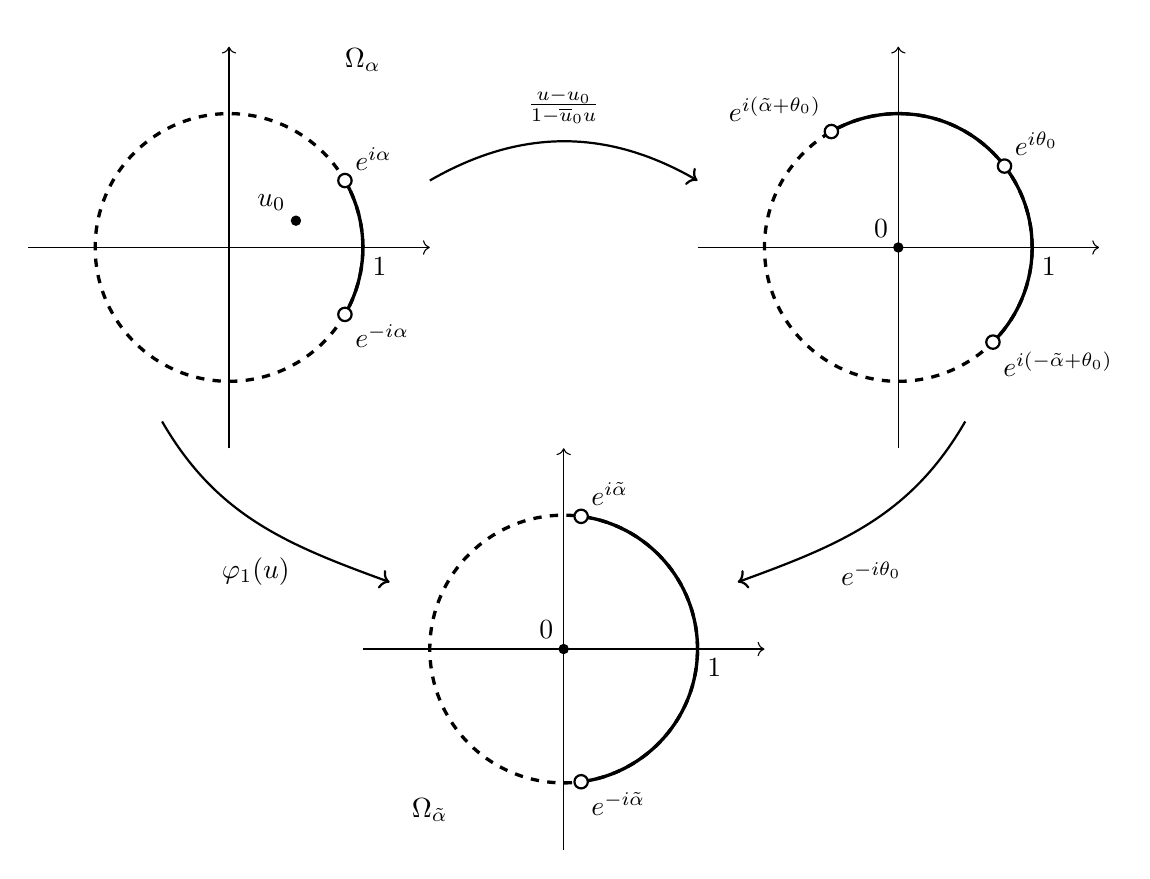
\begin{tikzpicture}[scale=1.7]

% Draw the codomain (C \setminus {z : |z|=1 and |arg z|<=alpha})
\begin{scope}
    % Draw partial circular arc |u|=1 from e^{-i alpha} to e^{i alpha}
    \draw[dashed, very thick] (1,0) arc[start angle=0, end angle=360, radius=1];
    \draw[very thick] (1,0) arc[start angle=0, end angle=30, radius=1];
    \draw[very thick] (1,0) arc[start angle=0, end angle=-30, radius=1];

    % Horizontal axis and labels
    \draw[->] (-1.5,0) -- (1.5,0) node[right] {};
    \draw[->] (0,-1.5) -- (0,1.5) node[above] {};
	% Points e^{i alpha} and e^{-i alpha}
	\draw[thick,fill=white] (0.866,0.5) circle(0.05)node[above right] {$e^{i\alpha}$};
    \draw[thick,fill=white] (0.866,-0.5) circle(0.05)node[below right] {$e^{-i\alpha}$};
    \draw[thick,fill=black] (0.5,0.2) circle(0.03) node[above left] {$u_0$};
%    \fill[black] (0.866,0.5) circle(0.03) node[above right] {$e^{i\alpha}$};
%    \fill[black] (0.866,-0.5) circle(0.03) node[below right] {$e^{-i\alpha}$};

    % Mark |u|=1 point
    \node[below right] at (1,0) {$1$};
	
    % Codomain label
    \node at (1,1.4) {$\Omega_\alpha$};
\end{scope}


% Draw the codomain (C \setminus {z : |z|=1 and |arg z|<=alpha})
\begin{scope}[xshift=5cm]
    % Draw partial circular arc |u|=1 from e^{-i alpha} to e^{i alpha}
    \draw[dashed, very thick] (1,0) arc[start angle=0, end angle=360, radius=1];
    \draw[very thick] (1,0) arc[start angle=0, end angle=120, radius=1];
    \draw[very thick] (1,0) arc[start angle=0, end angle=-45, radius=1];

    % Horizontal axis and labels
    \draw[->] (-1.5,0) -- (1.5,0) node[right] {};
    \draw[->] (0,-1.5) -- (0,1.5) node[above] {};
	% Points e^{i alpha} and e^{-i alpha}
	\draw[thick,fill=white] (-0.5,0.866) circle(0.05)node[above left] {$e^{i(\tilde \alpha+\theta_0)}$};
    \draw[thick,fill=white] (0.707,-0.707) circle(0.05)node[below right] {$e^{i(-\tilde \alpha+\theta_0)}$};
    \draw[thick,fill=white] (0.7933,0.608) circle(0.05)node[above right] {$e^{i\theta_0}$};
    \draw[thick,fill=black] (0,0) circle(0.03) node[above left] {$0$};
%    \fill[black] (0.866,0.5) circle(0.03) node[above right] {$e^{i\alpha}$};
%    \fill[black] (0.866,-0.5) circle(0.03) node[below right] {$e^{-i\alpha}$};

    % Mark |u|=1 point
    \node[below right] at (1,0) {$1$};
	
\end{scope}


% Arrows to represent the conformal map
\draw[->, thick] (1.5,0.5) to[out=30, in=150] (3.5,0.5);
%\draw[<-, thick] (2,-0.5) to[out=-30, in=-150] (3,-0.5);

% Map label
\node[above] at (2.5,0.85) {$\frac{u-u_0}{1-\overline{u}_0 u}$};
% Draw the codomain (C \setminus {z : |z|=1 and |arg z|<=alpha})
\begin{scope}[xshift = 2.5cm, yshift=-3cm]
    % Draw partial circular arc |u|=1 from e^{-i alpha} to e^{i alpha}
    \draw[dashed, very thick] (1,0) arc[start angle=0, end angle=360, radius=1];
    \draw[very thick] (1,0) arc[start angle=0, end angle=82.5, radius=1];
    \draw[very thick] (1,0) arc[start angle=0, end angle=-82.5, radius=1];

    % Horizontal axis and labels
    \draw[->] (-1.5,0) -- (1.5,0) node[right] {};
    \draw[->] (0,-1.5) -- (0,1.5) node[above] {};
	% Points e^{i alpha} and e^{-i alpha}
	\draw[thick,fill=white] (0.1305,0.9914) circle(0.05)node[above right] {$e^{i\tilde \alpha}$};
    \draw[thick,fill=white] (0.1305,-0.9914) circle(0.05)node[below right] {$e^{-i\tilde \alpha}$};
    \draw[thick,fill=black] (0,0) circle(0.03) node[above left] {$0$};
%    \fill[black] (0.866,0.5) circle(0.03) node[above right] {$e^{i\alpha}$};
%    \fill[black] (0.866,-0.5) circle(0.03) node[below right] {$e^{-i\alpha}$};

    % Mark |u|=1 point
    \node[below right] at (1,0) {$1$};
	\node at (-1,-1.2) {$\Omega_{\tilde \alpha}$};

\end{scope}

% Arrows to represent the conformal map
\draw[->, thick] (5.5,-1.3) to[out=-120, in=20] (3.8,-2.5);

%\draw[->, thick] (3.6,-0.5) to[out=-160, in=80] (3,-1.5);
% Map label
\node[above] at (4.8,-2.6) {$e^{-i\theta_0}$};

\draw[->, thick] (-0.5,-1.3) to[out=-60, in=160] (1.2,-2.5);
% Map label
\node[above] at (0.2,-2.6) {$\varphi_1(u)$};

\end{tikzpicture}
\end{center}

\caption{The transformation of the domain $\Omega_\alpha$ (top left) to $\Omega_{\tilde{\alpha}}$ (bottom). The mapping $\varphi_1$ sends $u_0$ to the origin.}
\label{fig:conformal_maps_1}
\end{figure}
%%%
These mappings are Möbius transformations with inverses
\begin{equation}
    \varphi_1^{-1}(v) = \frac{e^{i \theta_0}v + u_0}{1 + \overline{u}_0 e^{i \theta_0} v} \quad \mbox { and } \quad
    \varphi_2^{-1}(\zeta) = \frac{\zeta - \zeta_0}{\zeta - \overline{\zeta}_0}, \quad \text{where } \; \zeta_0 = i \tan(\tilde{\alpha}/{2}).
\end{equation}
Let $\phi(u) := (\varphi_2 \circ \varphi_1)(u)$, so that $\phi(u_0) = \varphi_2(0) = \zeta_0$. Applying the same transport argument as in Lemma \ref{lem:identification}, we obtain the relation
\begin{equation}
    R_n^{\Gamma_\alpha,w}\bigl(\phi^{-1}(\zeta), \phi^{-1}(\zeta_0)\bigr) w\bigl(\phi^{-1}(\zeta)\bigr) = R_n^{\sfA_0,W_n}(\zeta, \zeta_0) W_n(\zeta),
    \label{eq:residual_relation_auxiliary_domain}
\end{equation}
where the weight $W_n$ on $\Omega_0$ is given by
\begin{equation}
    W_n(\zeta) = e^{i \theta} (\zeta - \zeta_\infty)^{k - n} \prod_{j=1}^k (\zeta - \overline{\zeta}_j)^{-1},
    \label{eq:transferred_weight_2}
\end{equation}
with $\zeta_j = \phi(u_j)$, $\zeta_\infty = \overline{\zeta}_0 = -i \tan(\tilde{\alpha}/{2})$, and $\theta\in[0, 2\pi)$ chosen such that $W_n(\zeta_0) > 0$.
The asymptotics of $R_n^{\sfA_0, W_n}(\cdot, \zeta_0) W_n(\cdot)$ is provided by Proposition \ref{prop:asymptotics_of_real_problem}. Substituting this into \eqref{eq:residual_relation_auxiliary_domain}, we find that uniformly on compact subsets of $\Omega_0$,
\begin{equation}
    \lim_{n\rightarrow \infty}b_{\Omega_\alpha}\bigl(\phi^{-1}(\zeta),\infty\bigr)^nR_n^{\Gamma_\alpha,w}\bigl(\phi^{-1}(\zeta),u_0\bigr) = \frac{1}{2} \biggl(1+\frac{\zeta_0 \sqrt{\zeta^2-1}}{\zeta \sqrt{\zeta_0^2-1}}\biggr)\frac{b_{\Omega_0}(\zeta,0)}{b_{\Omega_0}(\zeta,\zeta_\infty)}F_w\bigl(\phi^{-1}(\zeta),u_0\bigr).
    \label{eq:auxilliary_limit}
\end{equation}
Here, the normalization ensures $b_{\Omega_0}(\zeta_0,0)>0$ and $b_{\Omega_0}(\zeta_0,\zeta_\infty)>0$.



To express this result in terms of the variable $z \in \Omega_0$, we recall the conformal map $u: \Omega_0 \to \Omega_\alpha$ defined in \eqref{eq:mobius_transformation}. Its inverse is given by
\begin{equation}
    u^{-1}(\xi) = i\tan(\alpha/{2})\frac{1+\xi}{1-\xi}.
\end{equation}
We then consider the automorphism $\Phi : \Omega_0 \to \Omega_0$ given by the composition
\begin{equation}
    \Phi = u^{-1} \circ \varphi_1^{-1} \circ \varphi_2^{-1}.
\end{equation}
We observe that $\Phi$ maps the real line to itself. Moreover, by construction, we have
\[
    \Phi(\zeta_0) = u^{-1}\Bigl(\varphi_1^{-1}\bigl(\varphi_2^{-1}(\zeta_0)\bigr)\Bigr) = u^{-1}\bigl(\varphi_1^{-1}(0)\bigr) = u^{-1}(u_0) = z_{u_0}.
\]
To determine the image of the origin, we calculate
\begin{align*}
	\Phi(0) & = \bigl( u^{-1}\circ\varphi_1^{-1}\bigr)(-1) 
	 = u^{-1}\left(\frac{u_0-e^{i\theta_0}}{1-\overline{u}_0e^{i\theta_0}}\right) \\
	& = i\tan\left(\frac{\alpha}{2}\right)\frac{1-\overline{u}_0e^{i\theta_0}+u_0-e^{i\theta_0}}{1-\overline{u}_0e^{i\theta_0}-u_0+e^{i\theta_0}}.
\end{align*}
Using Euler's formula and the definition of $x_0$ in \eqref{eq:x_0_def}, this simplifies to $\Phi(0) = x_0$. 
Since $\Phi$ is an automorphism of $\Omega_0$ mapping the origin to $x_0 \in (-1,1)$, it must be of the form
\begin{equation}
    \Phi(\zeta) = \frac{\zeta + x_0}{1 + x_0 \zeta}, \quad \mbox{ with inverse } \; \Phi^{-1}(z) = \frac{z - x_0}{1 - x_0 z}.
    \label{eq:Phi_def}
\end{equation}



\begin{figure}[h]
\begin{center}
\begin{tikzpicture}[scale=1.7]

% Draw the domain (C \setminus ((-\infty,-1] \cup [1,\infty)))
\begin{scope}
    % Horizontal axis and labels
    \draw[->] (-2,0) -- (2,0) node[right] {$\text{Re}(\zeta)$};
    \draw[->] (0,-2) -- (0,1.5) node[above] {$\text{Im}(\zeta)$};
    
    % Cuts on the real axis
    \draw[thick] (-2,0) -- (-1,0);
    \draw[thick] (1,0) -- (2,0);

    % Circles to represent the endpoints of the cuts
    \draw[thick,fill=white] (-1,0) circle(0.05);
    \draw[thick,fill=white] (1,0) circle(0.05);

    % Labels for the cuts
    \node[below] at (-1,-0.1) {$-1$};
    \node[below] at (1,-0.1) {$1$};
% Mark the point z_0 = i tan(alpha/2)
    \draw[thick,fill=black] (0,1) circle(0.05) node[right] {$\zeta_0 = i\tan(\tilde\alpha/{2})$};
    \draw[thick,fill=black] (0,-1) circle(0.05) node[right] {$\zeta_\infty=\overline\zeta_0$};
    \draw[thick,fill=black] (0,0) circle(0.05) node[above right] {$0$};
    	\draw[dashed, very thick] (0,-1) -- (0,1);
    % Domain label
    \node at (1.5,1.7) {$\Omega_0$};
\end{scope}

% Draw the codomain (C \setminus {z : |z|=1 and |arg z|<=alpha})
\begin{scope}[xshift=5cm]
    % Horizontal axis and labels
    \draw[->] (-2,0) -- (2,0) node[right] {$\text{Re}(z)$};
    \draw[->] (0,-1.5) -- (0,1.5) node[above] {$\text{Im}(z)$};

	\draw[dashed, very thick] (0.8,1) arc[start angle=150, end angle=210, radius=2];

	\draw[thick,fill=black] (0.5320508076,0) circle(0.05)node[above left] {$x_0$};
	\draw[thick,fill=black] (0.8,1) circle(0.05)node[above right] {$z_{u_0}$};
    \draw[thick,fill=black] (0.8,-1) circle(0.05)node[below right] {$\overline{z}_{u_0}$};
    
    % Cuts on the real axis
    \draw[thick] (-2,0) -- (-1,0);
    \draw[thick] (1,0) -- (2,0);
	
    % Circles to represent the endpoints of the cuts
    \draw[thick,fill=white] (-1,0) circle(0.05);
    \draw[thick,fill=white] (1,0) circle(0.05);

    % Labels for the cuts
    \node[below] at (-1,-0.1) {$-1$};
    \node[below] at (1,-0.1) {$1$};
% Mark the point z_0 = i tan(alpha/2)
    %\draw[thick,fill=black] (0,0.5) circle(0.03) node[right] {$z_0 = i\tan\frac{\alpha}{2}$};
    % Domain label
    \node at (1.5,1.7) {$\Omega_0$};
    
\end{scope}

% Arrows to represent the conformal map
\draw[->, thick] (2,0.5) to[out=30, in=150] (4,0.5);
%\draw[<-, thick] (2,-0.5) to[out=-30, in=-150] (3,-0.5);

% Map label
\node[above] at (2.9,0.9) {$\Phi(\zeta)$};
\end{tikzpicture}
\end{center}

\caption{The Möbius transformation $\Phi$ mapping the auxiliary parameter plane (left) to the original parameter plane (right). The map is determined by the correspondence of the points $0 \mapsto x_0$ and $\zeta_0 \mapsto z_{u_0}$.}
\label{fig:conformal_maps_2}
\end{figure}

Substituting $\zeta = \Phi^{-1}(z)$ into the terms of \eqref{eq:auxilliary_limit}, we compute
\begin{equation}
    \frac{\zeta_0 \sqrt{\zeta^2-1}}{\zeta \sqrt{\zeta_0^2-1}}
    = \frac{\Phi^{-1}(z_{u_0})\sqrt{\Phi^{-1}(z)^2-1}}{\Phi^{-1}(z)\sqrt{\Phi^{-1}(z_{u_0})^2-1}}
    = \frac{z_{u_0}-x_0}{\sqrt{z_{u_0}^2-1}}\frac{\sqrt{z^2-1}}{z-x_0}
    = s(z, z_{u_0}).
\end{equation}
Similarly, the ratio of Blaschke factors transforms as
\begin{equation}
    \frac{b_{\Omega_0}(\zeta,0)}{b_{\Omega_0}(\zeta,\zeta_\infty)}
    = \frac{b_{\Omega_0}\bigl(\Phi^{-1}(z), \Phi^{-1}(x_0)\bigr)}{b_{\Omega_0}\bigl(\Phi^{-1}(z),\Phi^{-1}(\overline {z}_{u_0})\bigr)}
    = \frac{b_{\Omega_0}(z,x_0)}{b_{\Omega_0}(z,\overline{z}_{u_0})}.
\end{equation}
Finally, noting that $\phi^{-1}(\zeta) = u(z)$, substituting these identities into \eqref{eq:auxilliary_limit} yields the desired asymptotic formula \eqref{eq:asymptotics_z_domain}.
\end{proof}




We summarize our findings for the domain $\Omega_\alpha$, presenting the results in a form consistent with \cite{eichinger17}. Recall the mapping \(\lambda : \Omega_\alpha \to \mathsf{S}_{\pi/4}\) defined in \eqref{la} by 
\begin{equation}
	\lambda(u) := \left(\frac{ue^{i\alpha}-1}{u-e^{i\alpha}}\right)^{1/4}.
	\label{eq:lambda}
\end{equation}

\begin{theorem}
	\label{thm:weighted_residual_asymptotics}
	Let $w$ be the weight function defined in \eqref{eq:weight_function_form}. For a fixed $u_0\in \D$, we have 
	\begin{multline}
	 \lim_{n\rightarrow \infty}b_{\Omega_\alpha}(u,\infty)^nR_n^{\Gamma_\alpha,w}(u,u_0) \\ = \frac{1}{2}\left(1+\frac{h(\lambda(u),\lambda(u_0))}{h(\lambda(u_0),\lambda(u_0))}\right) \frac{|\lambda(u_0)|^2 \bigl(\lambda(u)^2-|\lambda(u_0)|^2\bigr) \bigl(\lambda(u)^2+\lambda(u_0)^2\bigr)}{\lambda_0^2 \, \bigl(\lambda(u)^2+|\lambda(u_0)|^2\bigr) \bigl(\lambda(u)^2-\overbar{\lambda(u_0)^2}\bigr)} F_w(u,u_0)  \quad
		\label{eq:local_uniform_asymptotics}
	\end{multline}
	uniformly on compact subsets of $\Omega_\alpha$, where the auxiliary function $h$ is given by
    \begin{equation} \label{h}
    	h(\lambda,\lambda_0) = \frac{\lambda^2}{(\lambda^2-|\lambda_0|^2)(\lambda^2+|\lambda_0|^2)}.
    \end{equation}
\end{theorem}


\begin{proof}
The result follows by transferring \eqref{eq:asymptotics_z_domain} into the domain $\mathsf{S}_{\pi/4}$ of the variable $\lambda$. To this end, consider the Möbius transformation $g:\overline{\mathbb{C}} \to \overline{\mathbb{C}}$ defined by
\[
   g(z) = \frac{z-1}{z+1}, \quad \mbox{with inverse } \;
   g^{-1}(\xi) = \frac{1+\xi}{1-\xi}.
\]
Note that $g$ maps the domain $\Omega_0$ onto $\overline{\mathbb{C}} \setminus [0,\infty)$.
Additionally, let $\Phi$ be the automorphism of $\Omega_0$ defined in \eqref{eq:Phi_def}. Since $\Phi$ preserves the real line and $\Phi(\pm 1) = \pm 1$, the composition $g \circ \Phi \circ g^{-1}$ is a Möbius transformation that preserves the ray $[0,\infty)$ and fixes both $0$ and $\infty$. Consequently, it must be a scaling $\xi \mapsto r \xi$ for some $r>0$. Observing that $g(i\mathbb{R}) = \mathbb{T}$, we conclude that $(g \circ \Phi)(i\mathbb{R}) = r\mathbb{T}$. Since the parameters $z_{u_0}$, $x_0$, and $\overline{z}_{u_0}$ all lie on $\Phi(i\mathbb{R})$, their images under $g$ lie on the circle of radius $r$.

We define the function $v(z)$ by choosing a branch of $\sqrt{g(z)}$ that maps $\Omega_0$ conformally onto the upper half-plane. Consistent with our earlier choice of branch cuts along $\mathbb{R} \setminus (-1,1)$, we have the identities $\sqrt{\overline{z}-1} = -\overline{\sqrt{z-1}}$ and $\sqrt{\overline{z}+1} = \overline{\sqrt{z+1}}$. This implies the symmetry relation
\[
   v(\overline{z}) = -\overline{v(z)}.
\]
Setting $v_0 = v(z_{u_0})$, we thus have $v(\overline{z}_{u_0}) = -\overline{v}_0$. Furthermore, since $|g(x_0)| = |g(z_{u_0})|$ and $g(x_0)<0$, it follows that $v(x_0) = i|v_0|$. The mapping properties of $v$ are illustrated in Figure \ref{fig:v_map}.



\begin{figure}[h]
\begin{center}
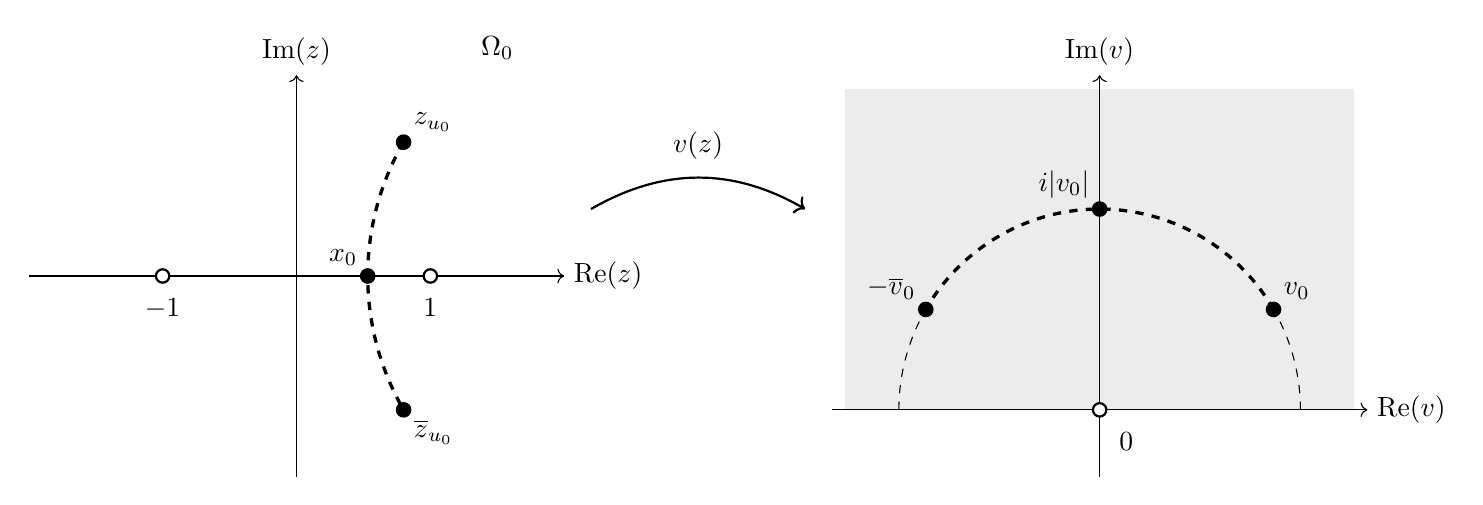
\begin{tikzpicture}[scale=1.7]

% Draw the codomain (C \setminus {z : |z|=1 and |arg z|<=alpha})
\begin{scope}
    % Horizontal axis and labels
    \draw[->] (-2,0) -- (2,0) node[right] {$\text{Re}(z)$};
    \draw[->] (0,-1.5) -- (0,1.5) node[above] {$\text{Im}(z)$};

	\draw[dashed, very thick] (0.8,1) arc[start angle=150, end angle=210, radius=2];

	\draw[thick,fill=black] (0.5320508076,0) circle(0.05)node[above left] {$x_0$};
	\draw[thick,fill=black] (0.8,1) circle(0.05)node[above right] {$z_{u_0}$};
    \draw[thick,fill=black] (0.8,-1) circle(0.05)node[below right] {$\overline{z}_{u_0}$};
    
    % Cuts on the real axis
    \draw[thick] (-2,0) -- (-1,0);
    \draw[thick] (1,0) -- (2,0);
	
    % Circles to represent the endpoints of the cuts
    \draw[thick,fill=white] (-1,0) circle(0.05);
    \draw[thick,fill=white] (1,0) circle(0.05);

    % Labels for the cuts
    \node[below] at (-1,-0.1) {$-1$};
    \node[below] at (1,-0.1) {$1$};
% Mark the point z_0 = i tan(alpha/2)
    %\draw[thick,fill=black] (0,0.5) circle(0.03) node[right] {$z_0 = i\tan\frac{\alpha}{2}$};
    % Domain label
    \node at (1.5,1.7) {$\Omega_0$};
    
\end{scope}

% Arrows to represent the conformal map
\draw[->, thick] (2.2,0.5) to[out=30, in=150] (3.8,0.5);


% Map label
\node[above] at (3.0,0.8) {$v(z)$};

% Draw the codomain (C \setminus {z : |z|=1 and |arg z|<=alpha})
\begin{scope}[xshift=6cm]
    % Horizontal axis and labels
     % Cuts on the real axis 
    %\draw[dashed, ultra thick] (-2,0) -- (2,0);
    
    % Fill the region between the lines with light gray
    \fill[gray!15] (-1.9,-1) -- (-1.9,1.4) -- (1.9,1.4) -- (1.9,-1) -- cycle;
    \draw[->] (-2,-1) -- (2,-1) node[right] {$\text{Re}(v)$};
    \draw[->] (0,-1.5) -- (0,1.5) node[above] {$\text{Im}(v)$};

	\draw[dashed, very thick] (1.5*0.866,-1.5*0.5+0.5) arc[start angle=30, end angle=150, radius=1.5];
	\draw[dashed, ] (1.5,-1) arc[start angle=0, end angle=30, radius=1.5];
	\draw[dashed, ] (-1.5,-1) arc[start angle=180, end angle=150, radius=1.5];

	\draw[thick,fill=black] (0,0.5) circle(0.05)node[above left] {$i|v_0|$};
	\draw[thick,fill=black] (1.5*0.866,-1.5*0.5+0.5) circle(0.05)node[above right] {$v_0$};
    \draw[thick,fill=black] (-1.5*0.866,-1.5*0.5+0.5) circle(0.05)node[above left] {$-\overline{v}_0$};
      
     \draw[thick,fill=white] (0,-1) circle(0.05);
	 \node[below] at (0.2,-1.1) {$0$};

    
\end{scope}
\end{tikzpicture}
\end{center}

\caption{The conformal map $v(z) = \sqrt{(z-1)/(z+1)}$ transforms the slit domain $\Omega_0$ (left) onto the upper half-plane (right). The points $z_{u_0}$, $\overline{z}_{u_0}$, and $x_0$ are mapped to $v_0$, $-\overline{v}_0$, and $i|v_0|$ respectively.}
\label{fig:v_map}
\end{figure}

Recall the mapping $\lambda(u)$ defined in \eqref{eq:lambda}. With $u(z)$ from \eqref{eq:mobius_transformation}, a direct computation shows that
\begin{equation}
   i\lambda\bigl( u(z) \bigr)^2 = v(z).
\end{equation}
With $\lambda = \lambda(u(z))$ and $\lambda_0 = \lambda(u_0)$, this identity implies $v(z) = i\lambda^2$ and $v_0 = i\lambda_0^2$.
We now rewrite the terms in the asymptotic formula \eqref{eq:asymptotics_z_domain} using these variables. Using the relation $z = g^{-1}(v^2)$ and recalling the definition of the $h$ in \eqref{h}, the term $s(z, z_{u_0})$ transforms as follows:
\begin{equation}
   s(z, z_{u_0}) = \frac{(v_0^2+|v_0|^2) v(z)}{v_0 (v(z)^2+|v_0|^2)} 
   = \frac{\lambda^2 (\lambda_0^2 - |\lambda_0|^2)(\lambda_0^2 + |\lambda_0|^2)}{\lambda_0^2 (\lambda^2 - |\lambda_0|^2)(\lambda^2 + |\lambda_0|^2)}
   = \frac{h(\lambda, \lambda_0)}{h(\lambda_0, \lambda_0)}.
\end{equation}
Similarly, the ratio of Blaschke factors becomes
\begin{equation}
	\frac{b_{\Omega_0}(z,x_0)}{b_{\Omega_0}(z,\overline{z}_{u_0})} 
    = i \frac{v(z)-i|v_0|}{v(z)+i|v_0|} \cdot \frac{|v_0|}{v_0}\frac{v(z)+v_0}{v(z)+\overline{v}_0} 
    = \frac{|\lambda_0|^2 (\lambda^2-|\lambda_0|^2) (\lambda^2+\lambda_0^2)}{\lambda_0^2 (\lambda^2+|\lambda_0|^2) (\lambda^2-\overbar{\lambda_0^2})}.
\end{equation}
Substituting these identities into \eqref{eq:asymptotics_z_domain} yields the formula \eqref{eq:local_uniform_asymptotics}, completing the proof.

\end{proof}



A central quantity of interest is the asymptotic extremal value at a given point $u_0$. To characterize this behavior, we set $\lambda = \lambda(u)$ and $\lambda_0 = \lambda(u_0)$, and introduce the kernel function $k_{\Omega_\alpha}$ defined by
\begin{equation}
	k_{\Omega_\alpha}(u,u_0) := k_{\C_+}\bigl(\lambda,\lambda_0\bigr)=\frac{2\lambda \overline{\lambda}_0 }{(\lambda+\overline{\lambda}_0)^2}.
\end{equation}
Recall that for the unweighted case ($w \equiv 1$), \cite{eichinger17} established that
\[\lim_{n\rightarrow \infty}e^{ng_{\Omega_\alpha}(u_0,\infty)}\|T_n^{\Gamma_\alpha}(\cdot,u_0)\| = \frac{1}{k_{\Omega_\alpha}(u_0,u_0)}.\]
We now extend this result to weighted residual polynomials with rational weights, paving the way for the broader class of admissible weight functions considered in the next section.


\begin{theorem}
	\label{thm:weighted_residual_asymptotics_at_point}
	Let $w$ be the weight function defined in \eqref{eq:weight_function_form}. Then for any point $u_0\in \Omega_\alpha$, we have 	
	\begin{equation}
		\lim_{n\rightarrow \infty}e^{ng_{\Omega_\alpha}(u_0,\infty)}\|wT_n^{\Gamma_{\alpha},w}(\cdot ,u_0)\|_{\Gamma_\alpha} = k_{\Omega_\alpha}(u_0,u_0)^{-1}\exp\left(\int_{\Gamma_\alpha}\log w(x)\,\omega(u_0,dx,\Omega_{\alpha})\right).
		\label{eq:residual_max_asymptotics}
	\end{equation}
\end{theorem}


\begin{proof}
First, assume that $u_0\in \D$. By the normalization in \eqref{normal}, we have $b_{\Omega_\alpha}(u_0,\infty) = e^{-g_{\Omega_\alpha}(u_0,\infty)}$. Hence, it follows from \eqref{eq:local_uniform_asymptotics} that as $n\rightarrow \infty$,
	\[
		e^{-n g_{\Omega_\alpha}(u_0,\infty)} R_n^{\Gamma_{\alpha},w}(u_0,u_0) \longrightarrow \frac{2|\lambda_0|^2}{(\lambda_0+\overline{\lambda}_0)^2} F_w(u_0,u_0) = k_{\Omega_\alpha}(u_0,u_0)F_w(u_0,u_0).
    \]
	Recalling that
	\[F_w(u_0,u_0) = \exp\left(-\int_{\Gamma_\alpha} \log w(x)\,\omega(u_0,dx,\Omega_{\alpha})\right),\]
	we obtain \eqref{eq:residual_max_asymptotics} as a direct consequence of the duality relation \eqref{eq:dual_relation}.
 

The corresponding result for the exterior $\{u: |u|>1\}$ follows from symmetry considerations. Let $u^\ast = 1/\overline{u}$. For $u_0\in \D$, the reflection formula \eqref{eq:reflection_formula} implies that
	\[
	e^{-ng_{\Omega_\alpha}(u_0^\ast,\infty)}R_{n}^{\Gamma_\alpha,w}(u_0^\ast,u_0^\ast) 
	= e^{-ng_{\Omega_\alpha}(u_0,\infty)}{R_{n}^{\Gamma_\alpha,w}(u_0,u_0)} 
	\longrightarrow k_{\Omega_\alpha}(u_0,u_0){F_w(u_0,u_0)}
	\]
	as $n\rightarrow \infty$. Since $\lambda(u^\ast) = \overline{\lambda(u)}$, we have $k_{\Omega_\alpha}(u_0^\ast,u_0^\ast) = k_{\Omega_\alpha}(u_0,u_0)$. Furthermore, since the weight $w$ is real-valued on $\Gamma_\alpha$, the Schwarz reflection principle implies that $F_w(u^\ast,u^\ast) = {F_w(u,u)}$. Thus, the limit holds for any $u_0^\ast$ in the exterior of the unit disk.
		


Finally, for $u_0\in \T\setminus \Gamma_\alpha$, we apply \cite[Lemma 2.7]{eichinger17}, suitably adjusted to the weighted setting. This ensures that the function
    \[
       u_0\longmapsto \lim_{n\rightarrow \infty} \Bigl( e^{ng_{\Omega_\alpha}(u_0,\infty)} \|wT_n^{\Gamma_\alpha, w}(\cdot,u_0)\|_{\Gamma_\alpha} \Bigr)
    \]
    is continuous on $\Omega_\alpha$, which completes the proof.	

\end{proof}
\begin{remark}
This result can naturally be interpreted through the theory of Hardy spaces. To describe how this is done, we let \(\Gamma\) denote a Jordan arc of class \(C^{1+\alpha}\) with complement \(\Omega\). If \(\psi\) denotes the conformal map from the exterior of the unit disk to \(\Omega\) mapping \(\infty\) to \(\infty\) then we let \(H^2(\Omega)\) consist of those functions \(F\) such that
\[F\circ \psi\in H^2(\bbD).\]
Such an \(F\) has non-tangential boundary values from either side (a.e. with respect to arc-length) on \(\Gamma\). We label these two boundary values by \(F_+\) and \(F_-\). Given a point \(z_0\in \Omega\), a norm on \(H^2(\Omega)\) is given by
\[\|F\|_{\omega(z_0)}^2= \int_{\Gamma}\bigl(|F_+(x)|^2+|F_-(x)|^2\bigr) \omega(z_0,dx,\Omega).\]
With this norm \(H^2(\Omega)\) becomes a reproducing kernel Hilbert space whose associated kernel is denoted by \(k_{\omega(z_0)}(z,\zeta)\). Classical Hilbert space theory shows that
\[\frac{1}{k_{\omega(z_0)}(z_0,z_0)} = \inf\left\{\int_{\Gamma}(|F_+(x)|^2+|F_-(x)|^2)\omega(z_0,dx,\Omega): F\in H^2(\Omega),\, F(z_0) = 1\right\}.\]
This quantity appears in relation to weighted residual polynomials through \cite[Conjecture 1.7]{buchecker-eichinger-zinchenko25} which hypothezises that if \(\Gamma\) is of class \(C^{1+\alpha}\) and \(w\) is an upper-semicontinuous weight function then
\[\lim_{n\rightarrow \infty}e^{ng_{\Omega}(z_0,\infty)}\|wT_n^{\Gamma,w}(\cdot,z_0)\|_{\Gamma} = \frac{1}{k_{\omega(z_0)}(z_0,z_0)}\exp\left(\int_{\Gamma}\log w(x)\omega(z_0,dx,\Omega_\alpha)\right).\]
In our current setting, where we investigate circular arcs, \cite[Theorem 5.4.10]{buchecker25} establishes the relation 
\[k_{\omega(u_0)}(u_0,u_0) = k_{\Omega_\alpha}(u_0,u_0).\]
Hence, Theorem \ref{thm:weighted_residual_asymptotics_at_point} proves the conjecture in the case of circular arcs and rational weights. Our aim is now to lift this result to a larger class of weight functions.
\end{remark}



\section{General Weight functions}
\label{sec:general_weight}
We now relax the assumptions on the weight function to extend formulas such as \eqref{eq:chebyshev_norm_asymptotics} to a broader class of weights. For clarity of presentation, we fix $u_0\in \Omega_\alpha=\overline{\C}\setminus \Gamma_\alpha$ and shift our focus from \(R_n^{\Gamma_\alpha,w}(\cdot,u_0)\) to \(T_n^{\Gamma_\alpha,w}(\cdot,u_0)=:T_n^{w}(\cdot,u_0)\). It should be stressed that, by \eqref{eq:chebyshev_residual_relation}, these are essentially the same object. 

To begin, let $w:\Gamma_\alpha\rightarrow (0,\infty)$ be a positive continuous function on $\Gamma_\alpha$. Suppose there exist polynomials $Q_1$ and $Q_2$, both nonvanishing on $\T$, such that
\begin{equation}
	\frac{1}{|Q_1(u)|}\leq w(u)\leq \frac{1}{|Q_2(u)|}
	\label{eq:polynomial_weight_inequalities}
\end{equation}
for all $u\in \Gamma_\alpha$. Then it is easily seen that
\begin{align} \notag
	\|T_n^{1/Q_1}(\cdot,u_0)/Q_1\|_{\Gamma_\alpha}&\leq \|T_n^{w}(\cdot,u_0)/Q_1\|_{\Gamma_\alpha}\leq \|w T_n^{w}(\cdot,u_0)\|_{\Gamma_\alpha}\\&\leq\|T_n^{1/Q_2}(\cdot,u_0)w\|_{\Gamma_\alpha}\leq \|T_n^{1/Q_2}(\cdot,u_0)/Q_2\|_{\Gamma_\alpha}.	
\end{align}
Without loss of generality, we may assume that the polynomials $Q_1$ and $Q_2$ have all their zeros in the set $\{u: |u|> 1\}$. To see that this assumption is non-restrictive, just observe that
\[
   |u-u_j| = |1-u\overline{u}_j| 
\]
for $u\in \T$. Consequently, if $P$ is a polynomial with a zero of order $n$ at $u_0\in \D$, the polynomial 
\[
   \frac{P(u)(1-u\overline{u}_0)^n}{(u-u_0)^n}
\] 
has the same absolute value on $\T$ but now has a zero at $1/\overline{u}_0$, which lies in the set $\{u: |u|>1\}$. 

Now, let $\epsilon>0$ be given. From Theorem \ref{thm:weighted_residual_asymptotics_at_point}, we have
\[\|T_n^{1/Q_k}(\cdot,u_0)/Q_k\|_{\Gamma_\alpha}\sim e^{-ng_{\Omega_\alpha}(u_0,\infty)}k_{\Omega_\alpha}(u_0,u_0)^{-1}\exp\left(-\int_{\Gamma_\alpha}\log Q_k(x)\,\omega(u_0,dx,\Omega_{\alpha})\right)\]
for $k\in \{1,2\}$.
%\[\|T_n^{1/Q_k}/Q_k\|_{\Gamma_\alpha}\sim 2\cos(\alpha/4)^2\Cap(\Gamma_\alpha)^n\exp\left(\int_{\Gamma_\alpha} -\log |Q_k(x)|d\mu_{\Gamma_\alpha}(x)\right\\]
By taking $n$ large enough, we can ensure that
\begin{multline*}
\qquad k_{\Omega_\alpha}(u_0,u_0)^{-1} \exp\left(-\int_{\Gamma_\alpha}\log Q_1(x)\,
\omega(u_0,dx,\Omega_{\alpha})\right)-\epsilon\leq 
\|w T_n^{w}(\cdot,u_0)\|_{\Gamma_\alpha}e^{ng_{\Omega_\alpha}(u_0,\infty)} \\
\leq k_{\Omega_\alpha}(u_0,u_0)^{-1}\exp\left(-\int_{\Gamma_\alpha}\log Q_2(x)\,\omega(u_0,dx,\Omega_{\alpha})\right)+\epsilon. \qquad	
\end{multline*}
Since $\epsilon>0$ was arbitrary, it follows that
\begin{multline}
k_{\Omega_\alpha}(u_0,u_0)^{-1}\exp\left(-\int_{\Gamma_\alpha}\log Q_1(x)\,
\omega(u_0,dx,\Omega_{\alpha})\right)
\leq \liminf_{n\rightarrow \infty} 
\|w T_n^{w}(\cdot,u_0)\|_{\Gamma_\alpha}e^{ng_{\Omega_\alpha}(u_0,\infty)}\label{eq:polynomial_approximation_above_below} \\
\leq \limsup_{n\rightarrow \infty} 
\|wT_n^{w}(\cdot,u_0)\|_{\Gamma_\alpha}e^{ng_{\Omega_\alpha}(u_0,\infty)} 
\leq k_{\Omega_\alpha}(u_0,u_0)^{-1}\exp\left(-\int_{\Gamma_\alpha}\log Q_2(x)\,
\omega(u_0,dx,\Omega_{\alpha})\right). %\notag
\end{multline}
%\begin{align}
%		\exp \left(\int_{\Gamma_\alpha} -\log |Q_1(x)|d\mu_{\Gamma_\alpha}(x)\right\}&\leq \liminf_{n\rightarrow \infty}\frac{\|T_n^{w}w\|_{\Gamma_\alpha}}{2\cos(\alpha/4)^2\Cap(\Gamma_\alpha)^n} 	\label{eq:polynomial_approximation_above_below}\\
%	\leq \limsup_{n\rightarrow \infty}&\frac{\|T_n^{w}w\|_{\Gamma_\alpha}}{2\cos(\alpha/4)^2\Cap(\Gamma_\alpha)^n}\leq \exp\left(\int_{\Gamma_\alpha} -\log |Q_2(x)|d\mu_{\Gamma_\alpha}(x)\right\} \notag
%\end{align}
This holds for any choice of polynomials $Q_1$ and $Q_2$ satisfying \eqref{eq:polynomial_weight_inequalities}. Our next step is to construct such polynomials so that the inequalities in \eqref{eq:polynomial_weight_inequalities} become approximate equalities.

Let $\epsilon>0$ be chosen such that $0<2\epsilon<\min_{u\in \Gamma_\alpha} w(u)$. By the Stone--Weierstra{\ss} theorem, we can approximate the function $1/w$ using polynomials in $u$ and $\overline{u}$. 
Specifically, there exist polynomials $P_1$ and $P_2$ satisfying
\begin{equation}
	w(u)-2\epsilon < 1/|P_{1}(u,\overline{u})|< w(u)-\epsilon\leq w(u)+\epsilon < 1/|P_2(u,\overline{u})|< w(u)+2\epsilon
	\label{eq:stone_weierstrass_generated_inequality}
\end{equation}
for all $u\in \Gamma_\alpha$. 
Since $\overline{u} = u^{-1}$ for $u\in \T$, the polynomials $P_k$ (for $k=1, 2$) can be rewritten as 
\[P_k(u,\overline{u}) = \sum_{l,j=1}^{m}a_{l,j}^{(k)}u^l\overline{u}^j = \sum_{l,j = 1}^{m}a_{l,j}^{(k)}u^lu^{-j} = u^{-m}\sum_{l,j=1}^{m}a_{l,j}^{(k)}u^{l}u^{m-j}\]
for $u\in \T$.
%As a consequence, the polynomials
Thus, defining
\[
	Q_{k}(u) := \sum_{l,j=1}^{m}a_{l,j}^{(k)}u^{l}u^{m-j},
\]
we obtain polynomials $Q_k$ whose absolute values on $\T$ coincide with those of $P_k$. 
%for $|u| = 1$ as the corresponding $P_{k}$'s. 
Moreover, we may assume that $Q_k$ is zero-free on $\T$. For if a zero appears, it can be perturbed by slightly dilating it with a factor $1+\delta$ (for some $\delta>0$), which continuously changes the modulus of the polynomial. If this perturbation is sufficiently small, the inequalities in \eqref{eq:stone_weierstrass_generated_inequality} remain valid, ensuring that
\begin{equation}
	w(u)-2\epsilon < 1/|Q_1(u)|< w(u)-\epsilon\leq w(u)+\epsilon < 1/|Q_2(u)|< w(u)+2\epsilon.
\end{equation}
Since this holds for all sufficiently small $\epsilon$, we can make the two integral in \eqref{eq:polynomial_approximation_above_below} arbitrarily close. 
This leads to the asymptotic formula
\begin{equation}
	\|w T_n^{w}(\cdot,u_0)\|_{\Gamma_\alpha}\sim  e^{-ng_{\Omega_\alpha}(u_0,\infty)}k_{\Omega_\alpha}(u_0,u_0)^{-1}\exp\left(\int_{\Gamma_\alpha} \log w(x)\,\omega(u_0,dx,\Omega_{\alpha})\right).
	\label{eq:limit_chebyshev_norm}
\end{equation}
%as $n\rightarrow \infty$.
%\begin{equation}
%	\lim_{n\rightarrow \infty}\frac{\|T_n^{w}w\|_{\Gamma_\alpha}}{2\cos(\alpha/4)^2\Cap(\Gamma_\alpha)^n}= \exp\left(\int_{\Gamma_\alpha} \log w(x)d\mu_{\Gamma_\alpha}(x)\right).
%	\label{eq:limit_chebyshev_norm}
%\end{equation}

By employing a similar approach, now approximating step functions from above and below, we can show that \eqref{eq:limit_chebyshev_norm} holds for any Riemann integrable weight function $w$ on $\Gamma_\alpha$ that satisfies the additional condition that there exists a constant $M\geq 1$ such that
\begin{equation}
	1/M\leq w(u)\leq M
	\label{eq:weight_bounds}
\end{equation}
for $u\in \Gamma_\alpha$.
%We refrain from providing these arguments as they are similar to those presented in \cite[Chapter I.7]{bernstein30}.
Since the necessary arguments closely follow those in \cite[Chapter I.7]{bernstein30} (see also \cite[Appendix A.2]{christiansen-eichinger-rubin23} for a summary), we omit them here.

%\begin{proposition}
%	Let $\E$ be a polynomially convex compact set and assume that for every positive upper-semicontinuous function $w_0:\E\rightarrow (0,\infty)$ it holds that
%	\begin{equation}
%		\|w_0T_n^{w_0}\|_{\E}\sim t_{\E}\Cap(\E)^n\exp\left(\int_{\E}\log w_0(x)d\mu_{\E}(x)\right)
%	\end{equation}
%	as $n\rightarrow\infty$ for some positive value $t_{\E}$. If $u_1,\dotsc,u_m$ is a collection of regular points (w.r.t potential theory) in $\partial\E \cap \operatorname{cvh}(\E)$ then for any collection $s_1\dotsc,s_m\in \R$ the weight $w(u) = w_0(u)\prod_{j=1}^{m}|u-u_j|^{s_j}$ satisfies
%	\begin{equation}
%		\|wT_n^{w}\|_{\E}\sim t_{\E}\Cap(\E)^n\exp\left(\int_{\E}\log w(x)d\mu_{\E}(x)\right)
%	\end{equation}
%	as $n\rightarrow \infty$.
%\end{proposition}
%\begin{proof}
%	We illustrate the inclusion of one zero of the weight so that in our assumptions we have $w(u) = w_0(u)|u-u_1|$. By rotating and translating the $u$-domain we may assume that $u_1 = 0$ and that $\E\subset \{u: \Im u\leq 0\}$. This changes the norm of the corresponding Chebyshev polynomial in the same way as it affects the capacity. The value of the logarithmic integral is further unchanged after precomposing the weight function with the inverse rotation and translation. 
%	
%	We initially assume that $s = 1$. By incorporating the zero of the weight $w$ into the polynomial we find that
%	\begin{align*}
%		\|T_{n}^{w}w\|_{\E}&\geq \|T_{n+1}^{w_0}w_0\|_{\E}\sim t_{\E}\Cap(\E)^{n+1}\exp\left(\int_{\E} \log w_0(x)d\mu_{\E}(x)\right).
%	\end{align*}
%	Frostman's Theorem \cite[Theorem 3.3.4]{ransford95} implies that
%	\begin{equation}
%		\int_{\E}\log |x|d\mu_{\E}(x)=\log \Cap(\E).
%		\label{eq:frostman}
%	\end{equation}
%	Therefore
%	\begin{equation}
%		\liminf_{n\rightarrow \infty}\frac{\|T_n^ww\|_{\E}}{\Cap(\E)^n}\geq t_{\E}\exp\left(\int_{\E} \log w(x)d\mu_{\E}(x)\right).
%		\label{eq:liminf_weight_zero}
%	\end{equation}
%	On the other hand by letting $w_\epsilon$ be defined by
%	\[w_\epsilon(u) = w_0(u)|u+i\epsilon |\]
%	we find that $w_\epsilon(u)>w(u)$ for any $u\in \E$ and furthermore $w_\epsilon$ satisfies the assumptions to ensure that \eqref{eq:chebyshev_norm_general_formula} holds. Consequently
%	\[\|T_n^{w}w\|_{\E}\leq \|T_n^{w_{\epsilon}}w_{\epsilon}\|_{\E}\sim t_{\E}\Cap(\E)^n\exp\left(\int_{\E}\log w_\epsilon(x)d\mu_{\E}(x)\right).\]
%	If we let $\epsilon\rightarrow 0$, the expression
%	\[\int_{\E}\log w_\epsilon(x)d\mu_{\E}(x) = \int_{\E}\log w_0(x)d\mu_{\E}(x)+\int_{\E}\log |x+i\epsilon|d\mu_{\E}(x)\]
%	converges by the monotone convergence theorem to
%	\[\int_{\E}\log w(x)d\mu_{\E}(x).\]
%	We find that 
%	\[\limsup_{n\rightarrow \infty}\frac{\|T_n^{w}w\|_{\E}}{\Cap(\E)^n}\leq t_\E\exp\left(\int_{\E}\log w(x)d\mu_{\E}(x)\right).\]
%	But this together with \eqref{eq:liminf_weight_zero} establishes that
%	\[		
%	\|T_n^{w}w\|_{\E}\sim t_\E\Cap(\E)^n\exp\left(\int_{\E} \log w(x)d\mu_{\E}(x)\right),
%	\]
%	as $n\rightarrow \infty$.
%	The use of induction extends \eqref{eq:chebyshev_norm_general_formula} to any weight of the form 
%	\[w(u) = w_0(u)|u|^m\]
%	when $m$ is a positive integer. If again $m$ is a positive integer but the weight satisfies
%	\[w(u) = w_0(u)|u|^{-m}\]
%	then it is clear that
%	\[|T_{n+m}^ww| =  |T_{n}^{w_0}w_0|\]
%	and so we again conclude the validity of \eqref{eq:chebyshev_norm_general_formula} from \eqref{eq:frostman}. To complete the proof we simply need to verify that \eqref{eq:chebyshev_norm_general_formula} holds for weights of the form 
%	\[w(u) = w_0(u)|u|^s\]
%	where $0<s<1$. For this reason we note that if $0<\delta<1$ we can define weight functions
%	\[w_l(u) = \begin{cases}
%		w_0(u)|u| & |u|<\delta\\
%%		w_0(u)|u|\frac{2\delta-|u|}{\delta} +w(u)\frac{|u|-\delta}{\delta} & \delta\leq |u|<2\delta\\
%		w(u) & |u|\geq \delta \\
%	\end{cases}\]
%	\[w_u(u) = \begin{cases}
%		w_0(u) & |u|<\delta\\
%%		w_0(u)\frac{2\delta-|u|}{\delta} +w(u)\frac{|u|-\delta}{\delta} & \delta\leq |u|<2\delta\\
%		w(u) & |u|\geq \delta \\
%	\end{cases}\]
%	then $w_l(u)\leq w(u)\leq w_u(u)$ holds throughout $\E$ and as a result
%	\[\|T_n^{w_l}w_l\|_{\E}\leq\|T_n^{w}w\|_{\E}\leq\|T_n^{w_u}w_u\|_{\E}.\]
%	We gather that
%	\begin{align*}
%		\exp\left(\int_{\E}\log w_l(x)d\mu_{\E}(x)\right)&\leq \liminf_{n\rightarrow\infty}\frac{\|T_n^{w}w\|_{\E}}{t_{\E}\Cap(\E)^n}\\
%		&\leq\limsup_{n\rightarrow\infty}\frac{\|T_n^{w}w\|_{\E}}{t_\E\Cap(\E)^n}\leq \exp\left(\int_{\E}\log w_u(x)d\mu_{\E}(x)\right).
%	\end{align*}
%	On the other hand we know that
%	\[\exp\left(\int_{\E}\log w_l(x)d\mu_{\E}(x)\right)\leq \exp\left(\int_{\E}\log w(x)d\mu_{\E}(x)\right) \leq \exp\left(\int_{\E}\log w_u(x)d\mu_{\E}(x)\right).\]
%	The monotone convergence theorem implies that if we let $\delta\rightarrow 0$ then the two extremals can be made arbitrarily close. The result now follows.
%
%\end{proof}

\subsection{Allowing for zeros}
The most general form of our asymptotic formula in the context of circular arcs is given as follows.

\begin{theoremm}
	Let $w:\Gamma_\alpha\rightarrow [0,\infty)$ be a weight function of the form
	\begin{equation}
	w(u) = w_0(u)\prod_{j=1}^{k}|u-u_j|^{s_j},
	\end{equation}
	where $w_0$ is a Riemann integrable function satisfying \eqref{eq:weight_bounds}, and where $u_j\in \Gamma_\alpha$ and $s_j\in \R$. Then, for any $u_0\in \Omega_\alpha$,
	\begin{equation}
		\|w T_n^{w}(\cdot,u_0)\|_{\Gamma_\alpha}\sim  e^{-ng_{\Omega_\alpha}(u_0,\infty)}k_{\Omega_\alpha}(u_0,u_0)^{-1}\exp\left(\int_{\Gamma_\alpha} \log w(x)\,\omega(u_0,dx,\Omega_{\alpha})\right).
	\end{equation}
%	as $n\rightarrow \infty$. 
	In particular,
	\begin{equation}
		\lim_{n\rightarrow \infty}\cW_n(\Gamma_\alpha,w)= 2\cos(\alpha/4)^2\exp\left(\int_{\Gamma_\alpha} \log w(x)\,d\mu_{\Gamma_\alpha}(x)\right).
		\label{eq:chebyshev_norm_general_formula}
	\end{equation}
	\label{thm:main_norm_asymptotics}
\end{theoremm}


\begin{proof}
	Similar to the approach in \cite{bernstein31}, we show how an additional factor $|u-u_j|^{s_j}$ can be incorporated into \eqref{eq:chebyshev_norm_general_formula}, under the assumption that \eqref{eq:chebyshev_norm_general_formula} holds for $w = w_0$. The remaining result can then be proved by induction. 
	
Let us begin by assuming that 
	\begin{equation}
	w(u) = w_0(u)|u-u_j|,
	\end{equation}
	where $w_0$ is a weight for which \eqref{eq:chebyshev_norm_general_formula} holds. 
	%as $n\rightarrow \infty$.	
	By incorporating the zero of the weight $w$ into the polynomial, we find that if $u_0\neq \infty$, then
	\begin{multline*}
		\qquad \frac{1}{|u_0-u_j|}\|w T_n^{w}(\cdot,u_0)\|_{\Gamma_\alpha}\geq \|w_0 T_{n+1}^{w_0}(\cdot,u_0)\| \\ \sim e^{-(n+1)g_{\Omega_\alpha}(u_0,\infty)}k_{\Omega_\alpha}(u_0,u_0)^{-1}\exp\left(\int_{\Gamma_\alpha} \log w_0(x)\,\omega(u_0,dx,\Omega_{\alpha})\right). \qquad
	\end{multline*}
	At the same time, it is clear that
	\[
		\|w T_n^{w}(\cdot,\infty)\|_{\Gamma_\alpha}\geq \|w_0 T_{n+1}^{w_0}(\cdot,\infty)\| \sim 2\cos(\alpha/4)^2\Cap(\Gamma_\alpha)^{n+1}\exp\left(\int_{\Gamma_\alpha} \log w_0(x)\,d\mu_{\Gamma_\alpha}(x)\right).
	\]
	The logarithmic integral of $w$ can be split into two parts:
	\[\int_{\Gamma_\alpha}\log w(x)\,\omega(u_0,dx,\Omega_\alpha) = \int_{\Gamma_\alpha}\log w_0(x)\,\omega(u_0,dx,\Omega_\alpha) +\int_{\Gamma_\alpha}\log |x-u_j|\,\omega(u_0,dx,\Omega_\alpha).\]
	%By applying Frostman's Theorem \cite[Theorem 3.3.4]{ransford95}, we see that
    By \cite[Sect.II.4]{ST97}, we see that
	\begin{equation}
		\exp\left(\int_{\Gamma_\alpha}\log |x-u_j|\,\omega(u_0,dx,\Omega_{\alpha})\right) = 
		|u_0-u_j| e^{-g_{\Omega_\alpha}(u_0,\infty)},
		%\exp\Bigl(\log|u_0-u_j|-g_{\Omega_\alpha}(u_0,\infty)\Bigr).
		\label{eq:frostman_theorem}
	\end{equation}
	which simplifies to $\Cap(\Gamma_\alpha)$ when $u_0=\infty$. This implies that for any $u_0\in \Omega_\alpha$, we have
	\begin{equation}
		\liminf_{n\rightarrow \infty} 
		\|w T_n^{w}(\cdot,u_0)\|_{\Gamma_{\alpha}}e^{ng_{\Omega_\alpha}(u_0,\infty)}
		\geq k_{\Omega_\alpha}(u_0,u_0)^{-1}
		\exp\left(\int_{\Gamma_\alpha} \log w(x)\,\omega(u_0,dx,\Omega_{\alpha})\right).
		\label{eq:liminf_weight_zero}
	\end{equation}
%	\begin{align*}
%		\|T_{n}^{w}w\|_{\Gamma_\alpha}&\geq \|T_{n+1}^{w_0}w_0\|_{\Gamma_\alpha}\sim 2\cos(\alpha/4)^2\Cap(\Gamma_\alpha)^{n+1}\exp\left(\int_{\Gamma_\alpha} \log w_0(x)d\mu_{\Gamma_\alpha}(x)\right).
%	\end{align*}
%	Frostman's Theorem, \cite[Theorem 3.3.4]{ransford95} implies that
%	\[\int_{\Gamma_\alpha}\log |u-x|d\mu_{\Gamma_\alpha}(x)=\log \Cap(\Gamma_\alpha),\]
%	in turn, allowing us to rewrite the inequality as
%	\begin{equation}
%		\liminf_{n\rightarrow \infty}\frac{\|T_n^ww\|_{\Gamma_\alpha}}{\Cap(\Gamma_\alpha)^n}\geq 2\cos(\alpha/4)^2\exp\left(\int_{\Gamma_\alpha} \log w(x)d\mu_{\Gamma_\alpha}(x)\right).
%		\label{eq:liminf_weight_zero}
%	\end{equation}
To estimate the corresponding $\limsup$, we define $w_\epsilon$ as
	\begin{equation}
	w_\epsilon(u) = w_0(u)(|u-u_j|+\epsilon),
	\end{equation}
	and observe that $w_\epsilon(u)>w(u)$ for any $u\in \Gamma_\alpha$. Additionally, $w_\epsilon$ satisfies the assumptions necessary to ensure that 
	%\eqref{eq:chebyshev_norm_general_formula} 
	\eqref{eq:limit_chebyshev_norm} holds. Consequently, we have
	\[
		\|w T_n^{w}(\cdot,u_0)\|_{\Gamma_\alpha}\leq \|w_{\epsilon} T_n^{w_{\epsilon}}(\cdot,u_0)\|_{\Gamma_\alpha}\sim e^{-ng_{\Omega_\alpha}(u_0,\infty)}k_{\Omega_\alpha}(u_0,u_0)^{-1}\exp\left(\int_{\Gamma_\alpha} \log w_{\epsilon}(x)\,\omega(u_0,dx,\Omega_{\alpha})\right).
	\]
%	\[\|T_n^{w}(\cdot,u_0)w\|_{\Gamma_\alpha}\leq \|T_n^{w_{\epsilon}}(\cdot,u_0)w_{\epsilon}\|_{\Gamma_\alpha}\sim 2\cos(\alpha/4)^2\Cap(\Gamma_\alpha)^n\exp\left(\int_{\Gamma_\alpha}\log w_\epsilon(x)d\mu_{\Gamma_\alpha}(x)\right).\]
	As $\epsilon\rightarrow 0$, the expression
	\[\int_{\Gamma_\alpha}\log w_\epsilon(x)\,\omega(u_0,dx,\Omega_{\alpha}) = \int_{\Gamma_\alpha}\log w_0(x)\,\omega(u_0,dx,\Omega_{\alpha})+\int_{\Gamma_\alpha}\log(|u-u_j|+\epsilon)\,\omega(u_0,dx,\Omega_{\alpha})\]
	converges, by the monotone convergence theorem, to
	\[\int_{\Gamma_\alpha}\log w(x)\,\omega(u_0,dx,\Omega_{\alpha}).\]
	We thus find that 
	\begin{equation}
	\limsup_{n\rightarrow \infty}
	   \|w T_n^{w}(\cdot,u_0)\|_{\Gamma_{\alpha}}e^{ng_{\Omega_\alpha}(u_0,\infty)}	   
	   \leq k_{\Omega_\alpha}(u_0,u_0)^{-1}
	   \exp\left(\int_{\Gamma_\alpha} \log w(x)\,\omega(u_0,dx,\Omega_{\alpha})\right).
	   \end{equation}
%	\[\limsup_{n\rightarrow \infty}\frac{\|T_n^{w}w\|_{\Gamma_\alpha}}{\Cap(\Gamma_\alpha)^n}\leq 2\cos(\alpha/4)^2\exp\left(\int_{\Gamma_\alpha}\log w(x)\omega(u_0,dx,\Omega_{\alpha})\right).\]
	Together with \eqref{eq:liminf_weight_zero}, this establishes that
	\begin{equation} \label{As}		
	\|w T_n^{w}(\cdot,u_0)\|_{\Gamma_\alpha}\sim  e^{-ng_{\Omega_\alpha}(u_0,\infty)}k_{\Omega_\alpha}(u_0,u_0)^{-1}\exp\left(\int_{\Gamma_\alpha} \log w(x)\,\omega(u_0,dx,\Omega_{\alpha})\right).
	\end{equation}
%	as $n\rightarrow \infty$.

The use of induction extends \eqref{As} to any weight of the form 
	\begin{equation} w(u) = w_0(u)|u-u_j|^m,\end{equation}
	where $m$ is a positive integer. Similarly, if $m$ is a positive integer and the weight has the form
	\[w(u) = w_0(u)|u-u_j|^{-m},\]
	it follows that
	\[T_{n+m}^w(u,u_0) =  \begin{cases}
	(u-u_j)^{m}(u_0-u_j)^{-m}T_{n}^{w_0}(u,u_0),& u_0\neq \infty, \vspace{0.15cm} \\ 
	\qquad \;(u-u_j)^{m}T_{n}^{w_0}(u,\infty), & u_0 = \infty. 
  \end{cases}
\]
	Hence, a brief computation confirms the validity of \eqref{As} in this case as well. 
	
	To complete the proof, it remains to verify that \eqref{As} holds for weights of the form 
	\begin{equation}w(u) = w_0(u)|u-u_j|^s,\end{equation}
	where $0<s<1$. To this end, we introduce the weight functions, parameterized by $\delta>0$:
	%we note that for $\delta>0$, we can define weight functions
	\[w_l(u) = \begin{cases}
		w_0(u)|u-u_j|, & |u-u_j|<\delta,\\
		\quad \; \; \, w(u), & |u-u_j|\geq \delta, \\
	\end{cases}\]
	and
	\[w_u(u) = \begin{cases}
		w_0(u), & |u-u_j|<\delta,\\
		\, w(u), & |u-u_j|\geq \delta. \\
	\end{cases}\]
	It is a simple matter to verify that $w_l(u)\leq w(u)\leq w_u(u)$ for all $u\in \Gamma_\alpha$ and, consequently, 
	\[\|w_l T_n^{w_l}(\cdot,u_0)\|_{\Gamma_\alpha}\leq\|w T_n^{w}(\cdot,u_0)\|_{\Gamma_\alpha}\leq\|w_u T_n^{w_u}(\cdot,u_0)\|_{\Gamma_\alpha}.\]
	From this, it follows that
	\begin{multline*}
		\quad k_{\Omega_\alpha}(u_0,u_0)^{-1}
		\exp\left(\int_{\Gamma_\alpha}\log w_l(x)\,\omega(u_0,dx,\Omega_{\alpha})\right)
		\leq \liminf_{n\rightarrow\infty}
		\|w T_n^{w}(\cdot,u_0)\|_{\Gamma_{\alpha}}e^{ng_{\Omega_\alpha}(u_0,\infty)} \\
	        \leq\limsup_{n\rightarrow\infty}
	        \|w T_n^{w}(\cdot,u_0)\|_{\Gamma_{\alpha}}e^{ng_{\Omega_\alpha}(u_0,\infty)}
	        \leq k_{\Omega_\alpha}(u_0,u_0)^{-1}
	        \exp\left(\int_{\Gamma_\alpha}\log w_u(x)\,\omega(u_0,dx,\Omega_{\alpha})\right). \quad
	\end{multline*}
	Since
	\[
	\int_{\Gamma_\alpha}\log w_l(x)\,\omega(u_0,dx,\Omega_{\alpha})
	\leq \int_{\Gamma_\alpha}\log w(x)\,\omega(u_0,dx,\Omega_{\alpha})
	\leq \int_{\Gamma_\alpha}\log w_u(x)\,\omega(u_0,dx,\Omega_{\alpha}),	
	\]
	the monotone convergence theorem implies that as $\delta\rightarrow 0$, the upper and lower bounds %become arbitrarily close. The result now follows.
	converge to the same limit. This completes the proof.
\end{proof}

Theorem \ref{thm:main_norm_asymptotics} provides an asymptotic formula for the weighted norm of a broad class of weighted Chebyshev polynomials on circular arcs. To our knowledge, this is the first example of such a result for Jordan arcs beyond the classical case of an interval.
%We wish to make a remark.

%\begin{remark}
Interestingly, the key argument that allows us to extend the result from positive continuous weights to weights with zeros is not specific to intervals or circular arcs; rather, it applies to any %sufficiently smooth 
Jordan arc and, in fact, to more general compact sets. More precisely, let $K$ be a regular (for potential theory) compact set for which there exists a constant $C_K$ such that
	\begin{equation} \label{W0}
	\lim_{n\rightarrow \infty}\cW_n(K,w_0)= 
	C_K\exp\left(\int_{K} \log w_0(x)\,d\mu_{K}(x)\right)
	\end{equation}
	for every continuous positive weight $w_0:K\to (0,\infty)$. Then the method used in the proof of Theorem \ref{thm:main_norm_asymptotics} can be adapted to show that \eqref{W0} remains valid for more general weights of the form
%	\[\lim_{n\rightarrow \infty}\cW_n(\Gamma,w)= C_\Gamma\exp\left(\int_{\Gamma} \log w(x)\,d\mu_{\Gamma}(x)\right)\]
	\begin{equation}
	   w(x) = w_0(x)\prod_{j=1}^{m}|x-x_j|^{s_j},
	\end{equation}   
	where $s_j\in \R$ and $x_j\in K$ for $j=1,\dots,m$.
    %lie on
	%$\Gamma \cap \partial\operatorname{cvh}(\Gamma)$ -- 
	%both $\Gamma$ and the boundary of the convex hull of $\Gamma$.
%\end{remark}


\section*{Acknowledgement}
These results were established during a SQuaRE meeting at the American Institute of Mathematics (AIM) in Pasadena, CA. We extend our heartfelt gratitude to AIM for their generous hospitality and for creating such an inspiring scientific environment.

\bibliographystyle{plain} % We choose the "plain" reference style
\begin{thebibliography}{10}

\bibitem{achieser56}
N.~I. Achieser.
\newblock {\em Theory of Approximation}.
\newblock Frederick Ungar publishing co. New York, 1956.

\bibitem{ahlfors78}
L.~V. Ahlfors.
\newblock {\em Complex Analysis}.
\newblock International Series in Pure and Applied Mathematics. McGraw--Hill Book Co., New York, 3rd edition, 1978.
\newblock An introduction to the theory of analytic functions of one complex variable.

\bibitem{alpan22}
G.~Alpan.
\newblock Extremal polynomials on a {J}ordan arc.
\newblock {\em J. Approx. Theory}, 276:105708, 2022.

\bibitem{armitage-gardiner01}
D.~Armitage and S.~J. Gardiner.
\newblock {\em Classical Potential Theory}.
\newblock Springer-Verlag, London, 2001.

\bibitem{bergman-rubin24}
A.~Bergman and O.~Rubin.
\newblock Chebyshev polynomials corresponding to a vanishing weight.
\newblock {\em J. Approx. Theory}, 301:106048, 2024.

\bibitem{bernstein30}
S.~N. Bernstein.
\newblock Sur les polyn\^{o}mes orthogonaux relatifs \`{a} un segment fini.
\newblock {\em J. Math.}, 90:127--177, 1930.

\bibitem{bernstein31}
S.~N. Bernstein.
\newblock Sur les polyn\^{o}mes orthogonaux relatifs \`{a} un segment fini (seconde partie).
\newblock {\em J. Math.}, 10:219--286, 1931.

\bibitem{buchecker25}
B.~Buchecker.
\newblock {\em Asymptotics of extremal polynomials on a {J}ordan curve or arc.}
\newblock Master's thesis,  Technische Universit\"{a}t Wien, 2025.

\bibitem{buchecker-eichinger-zinchenko25}
B.~Buchecker, B.~Eichinger, and M.~Zinchenko.
\newblock {Asymptotics of \(L^r\) extremal polynomials for \(0<r\leq \infty\) on \(C^{1+}\) {J}ordan regions}.
\newblock {\em \normalfont{{\bf arXiv} preprint}}, 2502.17616.

\bibitem{christiansen-eichinger-rubin23}
J.~S. Christiansen, B.~Eichinger, and O.~Rubin.
\newblock Extremal polynomials and sets of minimal capacity.
\newblock {\em Constr. Approx.}, 62:523--563, 2025.

\bibitem{christiansen-simon-zinchenko-II}
J.~S. Christiansen, B.~Simon, P~Yuditskii, and M.~Zinchenko.
\newblock {Asymptotics of {C}hebyshev polynomials, {II}: {DCT} subsets of ${\mathbb{R}}$}.
\newblock {\em Duke Math. J.}, 168(2):325--349, 2019.

\bibitem{christiansen-simon-zinchenko-I}
J.~S. Christiansen, B.~Simon, and M.~Zinchenko.
\newblock Asymptotics of {C}hebyshev polynomials, {I}. Subsets of {$\mathbb{R}$}.
\newblock {\em Invent. Math.}, 208:217--245, 2017.

\bibitem{christiansen-simon-zinchenko-V}
J.~S. Christiansen, B.~Simon, and M.~Zinchenko.
\newblock Asymptotics of {C}hebyshev polynomials, {V}. Residual polynomials.
\newblock {\em Ramanujan J.}, 61:251--278, 2023.

\bibitem{conway78}
J.~B. Conway.
\newblock {\em Functions of One Complex Variable I}.
\newblock Graduate texts in mathematics. Springer New York, 1978.

\bibitem{driscoll-toh-trefethen98}
T.~A. Driscoll, K.-C. Toh, and L.~N. Trefethen.
\newblock From potential theory to matrix iterations in six steps.
\newblock {\em SIAM Review}, 40:547--578, 1998.

\bibitem{eichinger17}
B.~Eichinger.
\newblock Szeg{\H{o}}--{W}idom asymptotics of {C}hebyshev polynomials on circular arcs.
\newblock {\em J. Approx. Theory}, 217:15--25, 2017.

\bibitem{fedorov85}
S.~I. Fedorov.
\newblock On a variational problem of {C}hebotarev in the theory of capacity of plane sets and covering theorems for univalent conformal mappings.
\newblock {\em Math. USSR Sbornik}, 52:115--133, 1985.

\bibitem{fischer96}
B.~Fischer.
\newblock {\em Polynomial Based Iteration Methods for Symmetric Linear Systems}.
\newblock Wiley, New York, 1996.

\bibitem{freund88}
R.~Freund.
\newblock On some approximation problems for complex polynomials.
\newblock {\em Constr. Approx.}, 4:111--121, 1988.

\bibitem{freund-ruscheweyh}
R.~Freund and S.~Ruscheweyh.
\newblock On a class of {C}hebyshev approximation problems which arise in connection with a conjugate gradient type method.
\newblock {\em Numer. Math.}, 48:525--542, 1986.

\bibitem{garnett-marschall05}
J.~B. Garnett and D.~E. Marshall.
\newblock {\em Harmonic Measure}.
\newblock New Mathematical Monographs. Cambridge University Press, 2005.

\bibitem{grotzsch30}
H.~Gr{\"{o}}tzsch.
\newblock {\"{U}ber ein Variationsproblem der konformen Abbildungen}.
\newblock {\em Ber. Verh. S\"{a}chs. Akad. Wiss. Leipzig Phys.-Math. Kl.}, 82:251--263, 1930.

\bibitem{he94}
M.~He.
\newblock The {F}aber polynomials for $m$-fold symmetric domains.
\newblock {\em J. Comput. Appl. Math.}, 54:313--324, 1994.

\bibitem{kuijlaars06}
A.~Kuijlaars.
\newblock Convergence analysis of {K}rylov subspace iterations with methods from potential theory.
\newblock {\em SIAM Review}, 48:3--40, 2006.

\bibitem{kuzmina80}
G.~V. Kuz'mina.
\newblock Moduli of families of curves and quadratic differentials.
\newblock {\em Tr. V. A. Steklov Mat. Inst. Akad. Nauk SSSR}, 139, 1980.

\bibitem{landkof72}
N.~S. Landkof.
\newblock {\em Foundations of Modern Potential Theory}.
\newblock Springer-Verlag, New York-Heidelberg, 1972.

\bibitem{lorentz86}
G.~G. Lorentz.
\newblock {\em Approximation of Functions}.
\newblock Chelsea publishing company, New York, 1986.

\bibitem{markoff16}
W.~Markoff.
\newblock {\"{U}ber Polynome, die in einem gegebenen Intervalle m\"{o}glichst wenig von Null abweichen.}
\newblock {\em Math. Ann.}, 77:213--258, 1916.

\bibitem{martinez-finkelshtein-rakhmanov11}
A.~Mart{\'i}nez-Finkelshtein and E.~A. Rakhmanov.
\newblock Critical measures, quadratic differentials, and weak limits of zeros of {S}tieltjes polynomials.
\newblock {\em Commun. Math. Phys.}, 302:53--111, 2011.

\bibitem{minadiaz06}
E.~{Mi{\~{n}}a-D\'{i}az}.
\newblock {\em Asymptotics for {F}aber polynomials and polynomials orthogonal over regions in the complex plane}.
\newblock PhD thesis, Vanderbilt University, 2006.

\bibitem{novello-schiefermayr-zinchenko21}
G.~Novello, K.~Schiefermayr, and M.~Zinchenko.
\newblock Weighted {C}hebyshev polynomials on compact subsets of the complex plane.
\newblock In {\em From operator theory to orthogonal polynomials, combinatorics, and number theory}, pages 357--370. Springer, 2021.

\bibitem{ortega-cerda-pridhnani08}
J.~Ortega-Cerd\'{a} and B.~Pridhnani.
\newblock The {P}olya--{T}chebotarov problem.
\newblock {\em \normalfont \textbf{arXiv}}, 0809.2483, 2008.

\bibitem{peherstorfer-steinbauer01}
F.~Peherstorfer and R.~Steinbauer.
\newblock Orthogonal and {$L_q$}-extremal polynomials on inverse images of polynomial mappings.
\newblock {\em J. Comput. Appl. Math.}, 127:297--315, 2001.

\bibitem{ransford95}
T.~Ransford.
\newblock {\em Potential Theory in the Complex Plane}.
\newblock London Mathematical Society Student Texts. Cambridge university press, 1995.

\bibitem{ST97}
E. B. Saff and V. Totik, 
\newblock \emph{Logarithmic potentials with external fields}.
\newblock Vol. 316. Grundlehren der mathematischen Wissenschaften [Fundamental Principles of Mathematical Sciences]. Appendix B by Thomas Bloom. Springer-Verlag, Berlin, 1997, xvi+505 pp.

\bibitem{schiefermayr14}
K.~Schiefermayr.
\newblock The {P}{\'o}lya--{C}hebotarev problem and inverse polynomial images.
\newblock {\em Acta Math. Hung.}, 142:80--94, 2014.

\bibitem{schiefermayr15}
K.~Schiefermayr.
\newblock Zolotarev's conformal mapping and {C}hebotarev's problem.
\newblock {\em Integral Transforms Spec. Funct.}, 26:118--133, 2015.

\bibitem{schiefermayr-zinchenko21}
K.~Schiefermayr and M.~Zinchenko.
\newblock Norm estimates for {C}hebyshev polynomials, {I}.
\newblock {\em J. Approx. Theory}, 265:105561, 2021.

\bibitem{smirnov-lebedev68}
V.~I. Smirnov and N.~A. Lebedev.
\newblock {\em Functions of a Complex Variable: Constructive Theory}.
\newblock The M.I.T. press, Massachusetts Institute of Technology, Cambridge, Massachusetts, 1968.

\bibitem{stahl85-1}
H.~Stahl.
\newblock Extremal domains associated with an analytic function, {I-II}.
\newblock {\em Complex Variables, Theory Appl.}, 4:311--324; 325--338, 1985.

\bibitem{stahl85-2}
H.~Stahl.
\newblock The structure of extremal domains associated with an analytic function.
\newblock {\em Complex Variables, Theory Appl.}, 4:339--354, 1985.

\bibitem{stahl12}
H.~Stahl.
\newblock Sets of minimal capacity and extremal domains.
\newblock {\em \normalfont{\textbf{arXiv}}}, 1205.3811, 2012.

\bibitem{thiran-detaille91}
J.-P. Thiran and C.~Detaille.
\newblock Chebyshev polynomials on circular arcs and in the complex plane.
\newblock In {\em Progress in Approximation Theory}, pages 771--786. Academic Press, Boston, MA, 1991.

\bibitem{ullman60}
J.~L. Ullman.
\newblock Studies in {F}aber polynomials. {I}.
\newblock {\em Trans. Am. Math. Soc.}, 94:515--528, 1960.

\bibitem{widom69}
H.~Widom.
\newblock Extremal polynomials associated with a system of curves in the complex plane.
\newblock {\em Adv. Math.}, 3:127--232, 1969.

\bibitem{yuditskii99}
P.~Yuditskii.
\newblock A complex extremal problem of {C}hebyshev type.
\newblock {\em J. Anal. Math.}, 77:207--235, 1999.

\end{thebibliography}
\end{document}







\section{Chebyshev polynomials on lemniscatic arcs}
\label{sec:chebyshev_polynomials_system_of_arcs}
To illustrate the applicability of Theorem \ref{thm:main_norm_asymptotics}, we derive asymptotic formulas for the Widom factors associated with a family of unions of arcs. These results complement the analysis in \cite{christiansen-eichinger-rubin23}. 

%Possible limit points of $\cW_n(\E,w)$ are well-understood in the case where $\E$ consists of unions of disjoint smooth Jordan curves. These results, due to Widom, can be found in \cite{widom69}. What turns out to be more elusive is the corresponding behavior of $\cW_n$ in relation to Jordan arcs. For such sets, Widom was not able to determine the asymptotical behavior for $\cW_n(\E,w)$ and he could only provide upper bounds. 

As previously mentioned, when $\Gamma$ is a smooth arc %with complement $\Omega_\Gamma = \RS \setminus \Gamma$, 
\[
\limsup_{n \to \infty} \cW_n(\Gamma, w) \leq 2 \exp\left(\int_{\Gamma} \log w(x) \, d\mu_\Gamma(x)\right),
\]  
with equality if and only if $\Gamma$ is a straight line segment. This result is rooted in the fact that a straight line segment is the only Jordan arc \(\Gamma\) satisfying 
\begin{equation} 
\frac{\partial g_{\Omega_\Gamma}}{\partial n_+}(z,\infty) = \frac{\partial g_{\Omega_\Gamma}}{\partial n_-}(z,\infty), \quad \Omega_\Gamma = \RS\setminus \Gamma
\label{eq:s-property-arc}
\end{equation} 
at all interior points. The generalization of \eqref{eq:s-property-arc} to a system of arcs is given by the following definition.

%As we preciously saw if $\Gamma$ is a smooth arc with complement $\Omega_\Gamma:= \RS\setminus \Gamma$ then
%\[\limsup_{n\rightarrow \infty}\cW_n(\Gamma,w)\leq 2 \exp\left(\int_{\Gamma}w(\zeta)d\mu_{\Gamma}(\zeta)\right)\]
%with equality if and only if \(\Gamma\) is a straight line segment. This has to do with the fact that a straight line segment is the only Jordan arc which has the property described in \eqref{eq:s-property-arc} whose generalization to a system of arcs is the following.

 \begin{definition}          
 \label{def:s-property}
        Let $\E\subset \C$ be a compact set with $\Cap(\E)>0$, and suppose that $\Omega_\E=\RS\setminus \E$ is connected. Additionally, assume there exists a subset $\E_0\subset \E$ with $\Cap(\E_0) = 0$, such that
        \begin{equation}
        	\E\setminus \E_0 = \bigcup_{i\in I}\Gamma_i,
        \end{equation}
        where the $\Gamma_i$'s are disjoint open analytic Jordan arcs, and $I\subset \N$. We say that $\E$ satisfies the $S$-property if
        \begin{equation}
			\frac{\partial g_{\Omega_\E}}{\partial n_+}(z,\infty)=\frac{\partial g_{\Omega_\E}}{\partial n_-}(z,\infty)
			\label{eq:s-property}
	\end{equation}
        holds for all $z\in \E\setminus \E_0$, where $n_+$ and $n_-$ denote the unit normals from each side of the arcs.
    \end{definition}
  
%{\color{red}{    
    The \(S\)-property is closely related to capacity minimization, and we refer the reader to \cite{stahl85-1,stahl85-2,stahl12} for further details on this. In \cite{christiansen-eichinger-rubin23}, the Chebyshev polynomials associated with the $m$-stars defined by $\E_m:=\{z:z^m\in [-2,2]\}$ are studied. These $m$-stars serve as examples of sets with the $S$-property, and it is shown that $\cW_n(\E_m)\rightarrow 2$ as $n\rightarrow \infty$ for any $m$. This behavior is analogous to that of Jordan arcs satisfying the $S$-property (i.e., straight line segments). %It is natural to speculate that minimal capacity sets -- i.e. sets which satisfy the $S$-property -- are related to large limits of Widom factors, presumably asymptotically equal to $2$ since all known limit points of $\{\cW_n(\E)\}$ related to compact connected sets $\E$ lie within $[1,2]$. 
 
     From the very definition in \eqref{eq:widom_factor}, one might expect that sets of minimal capacity yield large Widom factors, though the norms in the numerator also play a crucial role. The results of \cite{christiansen-eichinger-rubin23} suggest that the $S$-property is the key mechanism behind large limits of Widom factors, specifically leading to a limit of 2. To date, no known examples exist of connected sets for which $\limsup \mathcal{W}_n(\E) >2$. One might even conjecture that for connected sets, this $\limsup$ is always strictly less than $2$ unless the $S$-property holds.

     In this section, we provide evidence supporting the conjecture that the $S$-property is essential for obtaining large limits of Widom factor in the context of connected sets. To illustrate this, we examine a family of unions of arcs where the $S$-property fails and show that their corresponding Widom factors are asymptotically strictly less than 2.
    
%    It is natural to conjecture that minimal capacity sets--i.e., sets satisfying the $S$-property--are closely connected to large limits of Widom factors. Specifically, these factors are presumed to be asymptotically equal to $2$, as all known limit points of the sequence $\{\mathcal{W}_n(\E)\}$, associated with compact connected sets $\E$, lie within the interval $[1, 2]$. Indeed, from the definition \eqref{eq:widom_factor}, small capacities should give rise to large Widom factors, although the picture is made complicated by the dependence of the numerator. %In the present section we wish to provide evidence toward the fact that the $S$-property is related to large limits of Widom factors. We exemplify this by providing a family for which this condition fails and show that their related Widom factors are asymptotically strictly less than $2$.

%    In this section, we provide evidence supporting the conjecture that the $S$-property is essential for obtaining large limits of Widom factors in the setting of connected sets. To illustrate this, we examine a family of arc unions where the $S$-property fails and show that their corresponding Widom factors are asymptotically strictly less than 2.
%}}
    
%    Here we intend to show that weighted formulas such as \eqref{eq:chebyshev_norm_asymptotics} can be used to provide asymptotics of Widom factors corresponding to symmetric systems of arcs which do not satisfy the $S$-property. The computed limit points lie strictly between $1$ and $2$ for our examples.
%    As we will see, our computations of limits of Widom factors corresponding to certain families of sets which are not minimal capacity sets lie strictly between $1$ and $2$ in the limit.


    
\subsection{Lemniscatic arcs}
Extremal polynomials associated with lemniscates of the form $\{z:z^m+1\in r\T\}$, where $m\in \N$ and $r>0$, have been extensively studied in the literature (see e.g. \cite{bergman-rubin24, peherstorfer-steinbauer01, minadiaz06, ullman60, he94}). To obtain a system of arcs, we remove a segment of the circle and consider the following family
\begin{equation}
	\E_{m,r}(\alpha):=\{z: z^m+1\in r \Gamma_\alpha\},\quad 0<\alpha<\pi.
	\label{eq:def_lemniscatic_arc}
\end{equation}
Examples of such sets are shown in Figure \ref{fig:system_arcs}. 

\begin{figure}[h!]
	\centering
	\includegraphics[width = \textwidth]{Figures/system_arcs.png}
	\caption{Examples of sets in the families $\E_{2,r}(\pi/7)$, $\E_{5,r}(\pi/7)$ and $\E_{7,r}(\pi/7)$ for varying values of $r$. The critical case $r = 1$ is marked with a solid line.}
	\label{fig:system_arcs}
\end{figure}

With the help of \cite[Theorem 5.2.5]{ransford95}, we can immediately deduce that
\begin{equation}
	\Cap\bigl(\E_{m,r}(\alpha)\bigr) = \bigl(r\Cap(\Gamma_\alpha)\bigr)^{1/m}.
	\label{eq:lemniscatic_arcs_capacity}
\end{equation}
The sets in \eqref{eq:def_lemniscatic_arc} consist of \(m\) disjoint analytic arcs when \(r \neq 1\). However, if \(r = 1\), a crossing occurs at the origin where \(2m\) analytic arcs meet. As previously noted, it is known that 
\[
\limsup_{n \to \infty} \cW_n(\Gamma) < 2
\] 
for a smooth Jordan arc \(\Gamma\) that lacks the \(S\)-property, as proven in \cite{alpan22}. We will show that \(\E_{m,1}(\alpha)\) does not satisfy \eqref{eq:s-property}, making it particularly important to examine the asymptotic behavior of \(\cW_n(\E_{m,1}(\alpha))\). We hypothesize that the absence of the $S$-property for a connected system of arcs will result in the limit points of the associated Widom factors being strictly less than 2. If this assumption holds, we conclude that 
\[
\limsup_{n \to \infty} \cW_n\bigl(\E_{m,1}(\alpha)\bigr) < 2.
\] 
The primary goal of this section is to establish this result. To carry out the analysis, the asymptotics of the weighted Widom factors, as described in \eqref{eq:chebyshev_norm_asymptotics}, will play a central role. For the precise conditions required on the weight function $w$ for \eqref{eq:chebyshev_norm_asymptotics} to hold, we refer the reader to Theorem \ref{thm:main_norm_asymptotics}.

%To establish this is the primary goal of this section. In order to conduct the analysis, the asymptotics of the weighted Widom factors, as described in \eqref{eq:chebyshev_norm_asymptotics}, play a central role. We direct the reader to Theorem \ref{thm:main_norm_asymptotics} for the precise conditions required of the weight function \(w\) in order for \eqref{eq:chebyshev_norm_asymptotics} to hold. 

%{\color{red}{
In order to show that $\E_{m,1}(\alpha)$ does not satisfy \eqref{eq:s-property} at interior points of the subarcs, we utilize the connection to Chebotarev sets. Given $N$ distinct points $a_1\dotsc,a_N$ in the complex plane, there is a unique continuum (i.e., a compact connected set) of minimal logarithmic capacity containing these points. This set is known as the Chebotarev set for $\{a_1,\ldots,a_N\}$, with relevant references detailing its properties found in \cite{stahl12, grotzsch30, schiefermayr14, schiefermayr15, kuzmina80, fedorov85, martinez-finkelshtein-rakhmanov11, ortega-cerda-pridhnani08}. 
It is known (see \cite{stahl12}) that every Chebotarev set necessarily has the form specified in Definition \ref{def:s-property} and therefore satisfies the $S$-property. Moreover, the converse also holds, as can be inferred from the discussion following Problem 2 and Theorem 11 in \cite{stahl12}. In our case, this implies  the following: if $\E_{m,1}(\alpha)$ were to satisfy \eqref{eq:s-property} away from the points \(\{0\}\cup\{z: z^m+1\in e^{\pm i \alpha}\}\), it would necessarily coincide with the Chebotarev set associated with these points, excluding the point at zero.
%To begin, we show that $\E_{m,1}(\alpha)$ does not satisfy \eqref{eq:s-property} at interior points of its corresponding subarcs. Recall the Chebotarev problem: Given $N$ distinct points $a_1\dotsc,a_N$ in the complex plane, find the (as it turns out \cite{grotzsch30}) unique continuum (i.e. compact connected set) with minimal logarithmic capacity containing all points $a_1,\dotsc,a_N$. Relevant references detailing Chebotarev sets can be found in \cite{stahl12, schiefermayr14, schiefermayr15, kuzmina80, fedorov85, martinez-finkelshtein-rakhmanov11, ortega-cerda-pridhnani08}. It is known (see \cite{stahl12}) that such a set necessarily is of the form specified in Definition \ref{def:s-property} and so satisfies the $S$-property. Importantly, the converse also holds. See the discussion following Problem 2 as well as Theorem 11 in \cite{stahl12}. In our situation this entails that if $\E_{m,1}(\alpha)$ were to satisfy \eqref{eq:s-property} away from the points \(\{0\}\cup\{z: z^m+1\in e^{\pm i \alpha}\}\) then it would be the Chebotarev continuum corresponding to this set.
%}} 

\begin{proposition}
	For $0<\alpha<\pi$ and $m\in \N$, the set $\E_{m,1}(\alpha)$, as defined in \eqref{eq:def_lemniscatic_arc}, does not satisfy the $S$-property.
\end{proposition}
\begin{proof}
	The proof is carried out in a straight forward manner by showing that $\E_{m,1}(\alpha)$ is \emph{not} the Chebotarev set for the points 
	\[
	   \{z:z^m+1\in e^{\pm i\alpha}\}.
	\]    
To see this, let $\mathcal{C}(e^{\pm i\alpha}, 1)$ denote the Chebotarev set for $\{e^{\pm i\alpha}, 1\}$. By \cite[Theorem 1.2]{kuzmina80}, this set is necessarily contained within the convex hull of these points.
%Necessarily, $\mathcal{C}(e^{\pm i\alpha}, 1)$ is contained {\color{red} in the triangle with corners at $e^{\pm i\alpha}$ and $1$} (i.e., the convex hull of these points), see \cite[Theorem 1.2]{kuzmina80}. 
Since this does not hold for $\Gamma_\alpha$, we conclude that $\Gamma_\alpha\neq \mathcal{C}(e^{\pm i\alpha},1)$, which in turn implies 
	\[
	   \Cap(\Gamma_\alpha)>\Cap\bigl(\mathcal{C}(e^{\pm i\alpha},1)\bigr).
	\]    
Furthermore, the set $\{z: z^m+1\in \mathcal{C}(e^{\pm i\alpha}, 1)\}$ forms a continuum, %{\color{red}{
as $\mathcal{C}(e^{\pm i\alpha}, 1)$ contains the critical value of $z^m+1$. Applying \cite[Theorem 5.2.5]{ransford95} twice, we obtain
	\[
	\Cap\bigl(\{z:z^m+1\in \mathcal{C}(e^{\pm i\alpha},1)\}\bigr) = 
	\Cap\bigl(\mathcal{C}(e^{\pm i\alpha},1)\bigr)^{1/m} < 
	\Cap(\Gamma_\alpha)^{1/m} = 
	\Cap\bigl(\E_{m,1}(\alpha)\bigr).
	\]
Thus, \(\E_{m,1}(\alpha)\) is not the minimal capacity set containing \(\{z:z^m+1\in e^{\pm i\alpha}\}\) and consequently does not satisfy the $S$-property. % by \cite[Theorem 11]{stahl12}.
\end{proof}

We proceed by determining the limit points of the Widom factors associated with \(\E_{m,r}(\alpha)\). This set is invariant under rotations by \(2\pi/m\)-radians. As a result, the corresponding Chebyshev polynomial of degree \(nm + l\), where \(0 \leq l < m\), satisfies the symmetry relation 
\[
T_{nm+l}^{\E_{m,r}(\alpha)}(e^{2\pi i/m}z) = e^{2\pi il/m} T_{nm+l}^{\E_{m,r}(\alpha)}(z).
\]
This symmetry implies that all coefficients of \(T_{nm+l}^{\E_{m,r}(\alpha)}\), except those corresponding to terms of the form \(z^{l+km}\) with \(0 \leq k \leq n\), must vanish. Consequently, we have that
%
%The set $\E_{m,r}(\alpha)$ is invariant under rotations by $2\pi i/m$-radians. This has the effect that the Chebyshev polynomial of degree $nm+l$ where $0\leq l<m-1$ corresponding to $\E_{m,r}(\alpha)$ necessarily satisfies
%\[T_{nm+l}^{\E_{m,r}(\alpha)}(e^{2\pi i/m}z)=e^{2\pi il/m}T_{nm+l}^{\E_{m,r}(\alpha)}(z).\]
%Consequently, all coefficients of $T_{nm+l}^{\E_{m,r}(\alpha)}$ except possibly those corresponding to terms $z^{l+km}$ with $0\leq k\leq n$ must vanish. This implies that
\begin{equation}
	T_{nm+l}^{\E_{m,r}(\alpha)}(z) = z^lQ_n(z^m+1),
	\label{eq:cheb_on_lemniscatic_arcs_symmetry}
\end{equation}
where \(Q_n\) is a monic polynomial of degree \(n\). By applying the change of variables $z = (r\zeta-1)^{1/m}$, we obtain
\begin{equation}
	\max_{z\in \E_{m,r}(\alpha)}\left|T_{nm+l}^{\E_{m,r}(\alpha)}(z)\right| = 
	\max_{\zeta\in \Gamma_\alpha}\left|(r\zeta-1)^{l/m}\tilde{Q}_n(\zeta)r^n\right|,
	\label{eq:cheb_on_lemniscatic_arcs_weight}
\end{equation}
where $\tilde{Q}_n$ is the monic polynomial of degree $n$ that minimizes the norm on $\Gamma_\alpha$ with respect to the weight function $w_{r,m,l}:\Gamma_\alpha\rightarrow [0,\infty)$, given by 
\begin{equation}
	w_{r,m,l}(\zeta) = |r\zeta-1|^{l/m}.
\end{equation} 
In other words,
\begin{equation}
	\tilde{Q}_n(\zeta) =  T_{n}^{\Gamma_\alpha, w_{r,m,l}}(\zeta)=:T_{n}^{w_{r,m,l}}(\zeta),
	\label{eq:cheb_on_lemniscatic_arcs_weight_relation}
\end{equation}
and from \eqref{eq:cheb_on_lemniscatic_arcs_weight}, it follows that
\[\|T_{nm+l}^{\E_{m,r}(\alpha)}\|_{\E_{m,r}(\alpha)} = r^n\|w_{r,m,l}T_n^{w_{r,m,l}}\|_{\Gamma_\alpha}.\]
The asymptotic behavior of the right-hand side is given by \eqref{eq:chebyshev_norm_asymptotics}, or more precisely, by Theorem \ref{thm:main_norm_asymptotics}, which yields
\begin{equation}
	\|w_{r,m,l}T_n^{w_{r,m,l}}\|_{\Gamma_\alpha}\sim 2\cos(\alpha/4)^2\Cap(\Gamma_\alpha)^n\exp\left(\int_{\Gamma_\alpha}w_{r,m,l}(\zeta)\,d\mu_{\Gamma_\alpha}(\zeta)\right).
	\label{eq:cheb_on_lemniscatic_arcs_weight_asymptotics}
\end{equation}
In order to determine the asymptotics of $\cW_{n}(\E_{m,r}(\alpha))$, we must evaluate the integral on the right-hand side of \eqref{eq:cheb_on_lemniscatic_arcs_weight_asymptotics}. We isolate this computation as a lemma.
\begin{lemma}
	For $r>0$, the expression
\begin{equation}
   \exp\left(\frac{2m}{l}\int_{\Gamma_\alpha}\log w_{r,m,l}(\zeta)\,d\mu_{\Gamma_\alpha}(\zeta)\right)
\end{equation} 
evaluates to
	\begin{equation}
		 \frac{r^2+1}{2}-r\cos^2(\alpha/2)+\sqrt{\left(\frac{r^2+1}{2}-r\cos^2(\alpha/2)\right)^2-r^2\sin^4(\alpha/2)}.
\end{equation}
For $r=1$, this simplifies to $\Cap(\Gamma_\alpha)^{2} = \sin^2(\alpha/2)$.
\label{lem:logarithmic_integral}
\end{lemma}

As a consequence of \eqref{eq:lemniscatic_arcs_capacity}--\eqref{eq:cheb_on_lemniscatic_arcs_weight_asymptotics}, we obtain
\[
	\cW_{nm+l}\bigl(\E_{m,r}(\alpha)\bigr) = 
	\frac{\|w_{r,m,l}T_{n}^{w_{r,m,l}}\|_{\Gamma_\alpha}r^n}{\Cap\bigl(\E_{m,r}(\alpha)\bigr)^{nm+l}} = 
	\frac{\|w_{r,m,l}T_{n}^{w_{r,m,l}}\|_{\Gamma_\alpha}r^n}{\bigl(r\Cap(\Gamma_\alpha)\bigr)^{n+l/m}} 
\]
which tends to
\[	
   \frac{2\cos^2(\alpha/4)}{\bigl(r\Cap(\Gamma_\alpha)\bigr)^{l/m}}\exp\left(\frac{l}{m}\int_{\Gamma_\alpha}\log |r\zeta-1|\,d\mu_{\Gamma_\alpha}(\zeta)\right)
\]
as $n\rightarrow \infty$. Lemma \ref{lem:logarithmic_integral} then implies that
\begin{multline}
\lim_{n\rightarrow \infty}\cW_{nm+l}\bigl(\E_{m,r}(\alpha)\bigr) = \\  
2\cos^2(\alpha/4)\left(\frac{\frac{r^2+1}{2}-r\cos^2(\alpha/2)+\sqrt{\left(\frac{r^2+1}{2}-r\cos^2(\alpha/2)\right)^2-r^2\sin^4(\alpha/2)}}{r^2\sin^2(\alpha/2)}\right)^{\frac{l}{2m}}.  \quad
\end{multline}
For the special case $r = 1$, we observe that
\begin{equation}
   \cW_{n}\bigl(\E_{m,1}(\alpha)\bigr)\rightarrow 2\cos^2(\alpha/4) \; \text{ as }n\rightarrow \infty,
\end{equation}   
which matches the asymptotic behavior for $\cW_n(\Gamma_\alpha)$. In particular, this shows that
\[\limsup_{n\rightarrow \infty}\cW_n\bigl(\E_{m,1}(\alpha)\bigr)<2\]
for any $m$, complementing \cite[Theorem 1.2]{christiansen-eichinger-rubin23}, where a family of sets satisfying the $S$-property was shown to have Widom factors converging to $2$. 

We summarize our findings in the following theorem.

\begin{theorem} 	
\label{thm:Widom_factors_lemniscatic_arcs}
	Let $\E_{m,r}(\alpha)=\{z: z^m+1\in r \Gamma_\alpha\}$, where $m\in \N$, $r>0$, and $0<\alpha<\pi$. Then, for any $0\leq l <m$, we have
\begin{equation}
   \lim_{n\rightarrow \infty}\cW_{nm+l}\bigl(\E_{m,r}(\alpha)\bigr) = 2\cos^2(\alpha/4)\, c(r,\alpha)^{\frac{l}{2m}}
\end{equation}   
	where
\begin{equation}
c(r,\alpha)=\frac{\frac{r^2+1}{2}-r\cos^2(\alpha/2)+\sqrt{\left(\frac{r^2+1}{2}-r\cos^2(\alpha/2)\right)^2-r^2\sin^4(\alpha/2)}}{r^2\sin^2(\alpha/2)}.
\end{equation}
	In particular, for $r = 1$ we obtain
\begin{equation}
\lim_{n\rightarrow \infty}\cW_n\bigl(\E_{m,1}(\alpha)\bigr) = 2\cos^2(\alpha/4).
\end{equation}
\end{theorem}

\subsection{Analysis of the Limit Points}
It is illuminating to examine the range of the limit points for different values of $r$. The key is to understand the behavior of the function $r\mapsto c(r,\alpha)$ for a fixed $\alpha\in (0,\pi)$. Since $c(r,\alpha)>0$, the sign of $\partial_rc(r,\alpha)$ coincides with that of the logarithmic derivative $\partial_r c(r,\alpha)/c(r,\alpha)$, which is given by
	\begin{equation}
		\frac{
\Bigl( r\bigl(1+\cos(\alpha)\bigr) - 2 \Bigr) \sqrt{\left( r - 1 \right)^2 \bigl( -2r\cos(\alpha) + r^2 + 1 \bigr)} 
+ \left( r - 1 \right) \Bigl( ( r^2 - 3r )\cos(\alpha) + r^2 - r + 2 \Bigr)
}{
\sqrt{\left( r - 1 \right)^2 \bigl( -2r\cos(\alpha) + r^2 + 1 \bigr)} 
\, r \biggl( r^2 - \bigl(1+\cos(\alpha)\bigr)r + \sqrt{\left( r - 1 \right)^2 \bigl( -2r\cos(\alpha) + r^2 + 1 \bigr)} + 1 \biggr)
}.
\label{eq:log_derivative}
	\end{equation}
Therefore, $\partial_r c(r,\alpha)$ vanishes only if the numerator of \eqref{eq:log_derivative} is equal to $0$.
%\begin{align*}
%\left( r\Bigl(1+\cos(\alpha)\Bigr) - 2 \right) \sqrt{\left( r - 1 \right)^2 \left( -2r\cos(\alpha) + r^2 + 1 \right)} 
%+ \left( r - 1 \right) \Bigl( \left( r^2 - 3r \right)\cos(\alpha) + r^2 - r + 2 \Bigr) = 0.
%\end{align*}
%On the other hand, if this term vanishes then
Equivalently,
\begin{equation}
%	\left( r\Bigl(1+\cos(\alpha)\Bigr) - 2 \right)^2 \left( r - 1 \right)^2 \left( -2r\cos(\alpha) + r^2 + 1 \right) 
%\left( r - 1 \right)^2 \Bigl( \left( r^2 - 3r \right)\cos(\alpha) + r^2 - r + 2 \Bigr)^2 	\\
%\Leftrightarrow
2(r-1)^2 r^3 \bigl(-1+\cos(\alpha)\bigr)\sin(\alpha)^2 = 0,
\end{equation}
which holds if and only if $\alpha = \pi k$ for $k\in \Z$ or $r\in \{0,1\}$. In our setting, where $\alpha\in (0,\pi)$ and $r\notin\{0,1\}$, the derivative does not vanish anywhere. By the intermediate value theorem, $r\mapsto\partial_r c(r,\alpha)$ has a constant sign on $(0,1)$ and $(1,\infty)$, respectively. We conclude that $\partial_r c(r,\alpha)$ is negative for $0<r<1$ and positive for $r>1$. 

Moreover, since 
\[
   \lim_{r\rightarrow 0}c(r,\alpha) = \infty
     \quad \mbox{and} \quad
   \lim_{r\rightarrow \infty}c(r,\alpha) = \frac{1}{\sin^2(\alpha/2)},
\] 
it follows that $c(\cdot,\alpha)$ maps $(0,1)$ onto $(1,\infty)$ and $(1,\infty)$ onto $\bigl(1,1/\sin^2(\alpha/2)\bigr)$. Consequently, for $0\leq l<m$, we have
\[\lim_{n\rightarrow \infty}\cW_{nm+l}\bigl(\E_{m,r}(\alpha)\bigr) \in \begin{cases}
	[2\cos^2(\alpha/4),2\cos^2(\alpha/4)\sin^{-\frac{l}{m}}(\alpha/2)],& r> 1, \vspace{.3cm}\\
	\qquad\qquad\quad [2\cos^2(\alpha/4),\infty),& 0<r<1.
\end{cases}
\]

As mentioned earlier, the proof of Theorem \ref{thm:Widom_factors_lemniscatic_arcs} relies on the formula \eqref{eq:chebyshev_norm_asymptotics}, which we will establish in the remainder of this article. Theorem \ref{thm:Widom_factors_lemniscatic_arcs} in particular shows that the limit of $\cW_n(\E_{m,1}(\alpha))$ (i.e., in the connected case) always lies within the interval $(1,2)$. Furthermore, as $\E_{m,1}(\alpha)$ increasingly resembles a set of intersecting straight lines as $\alpha\rightarrow 0$, the corresponding value of $\lim_{n\rightarrow \infty}\cW_n(\E_{m,1}(\alpha))$ approaches $2$. This behavior should be compared with \cite[Theorem 1.2]{christiansen-eichinger-rubin23}.

